\documentclass[masc,oneside,12pt]{ubcthesis}%msc, phd, masc, ma, or meng


%%%%%%%%%%%%%%%%%%%%%%%%%%%%%%%%%%%%%%%%%%%%%%%%%%%%%%%%%%%%%%%%%%%%%%%%%%%%%%%%%%%%%%%%%
%      ╭━━━┳━━━┳━━━┳━╮╱╭┳━━━━╮╭━━━┳━━━┳━━━┳━━━╮
%      ┃╭━━┫╭━╮┃╭━╮┃┃╰╮┃┃╭╮╭╮┃┃╭━╮┃╭━╮┃╭━╮┃╭━━╯
%      ┃╰━━┫╰━╯┃┃╱┃┃╭╮╰╯┣╯┃┃╰╯┃╰━╯┃┃╱┃┃┃╱╰┫╰━━╮
%      ┃╭━━┫╭╮╭┫┃╱┃┃┃╰╮┃┃╱┃┃╱╱┃╭━━┫╰━╯┃┃╭━┫╭━━╯
%      ┃┃╱╱┃┃┃╰┫╰━╯┃┃╱┃┃┃╱┃┃╱╱┃┃╱╱┃╭━╮┃╰┻━┃╰━━╮
%      ╰╯╱╱╰╯╰━┻━━━┻╯╱╰━╯╱╰╯╱╱╰╯╱╱╰╯╱╰┻━━━┻━━━╯
%      
%%%%%%%%%%%%%%%%%%%%%%%%%%%%%%%%%%%%%%%%%%%%%%%%%%%%%%%%%%%%%%%%%%%%%%%%%%%%%%%%%%%%%%%%%


\institution{The University Of British Columbia}
\faculty{THE COLLEGE OF GRADUATE STUDIES}
\institutionaddress{Okanagan}



\title{A Broadband Fixed-beam Leaky-wave Antenna Based on Transformation Electromagnetics}
%\subtitle{With a Subtitle}
\author{Asif Al Noor} 
\copyrightyear{2016}
\submitdate{October 2016} % date of approved thesis
\program{Electrical Engineering}%or Mathematics, or Interdisciplinary Studies
%\previousdegree{B.Sc., Islamic University of Technology, 2013}

% ================================================================================


\usepackage{ubcostyle} %loads packages


% ===================================================================
% CHANGE THE FOLLOWING COMMANDS ACCORDING TO YOUR NEEDS
% ===================================================================
\newcommand{\R}{\mathbb{R}}   %real number
\newcommand{\Z}{\mathbb{Z}}   %integers
\newcommand{\C}{\mathbb{C}}   %complex numbers

\newcommand{\dom}{\operatorname{dom}}
\providecommand{\TT}[1]{\Theta\left(#1\right)} % big-Theta
\providecommand{\OO}[1]{\mathcal{O}\left(#1\right)} % big-Oh

%%%%%%%%%%%%%%%%%%%%%%%%%%%%%%%%%%%%%%%%%%%%%%%%%%%%%%%%%%%%%%%%%%%%%%%%%%%%%%%%%%%%%%%%%
%      ╭━━━━┳╮╱╭┳━━━┳━━━┳━━┳━━━╮╭━━╮╭━━━┳━━━┳╮╱╱╭╮
%      ┃╭╮╭╮┃┃╱┃┃╭━━┫╭━╮┣┫┣┫╭━╮┃┃╭╮┃┃╭━╮┣╮╭╮┃╰╮╭╯┃
%      ╰╯┃┃╰┫╰━╯┃╰━━┫╰━━╮┃┃┃╰━━╮┃╰╯╰┫┃╱┃┃┃┃┃┣╮╰╯╭╯
%      ╱╱┃┃╱┃╭━╮┃╭━━┻━━╮┃┃┃╰━━╮┃┃╭━╮┃┃╱┃┃┃┃┃┃╰╮╭╯
%      ╱╱┃┃╱┃┃╱┃┃╰━━┫╰━╯┣┫┣┫╰━╯┃┃╰━╯┃╰━╯┣╯╰╯┃╱┃┃
%      ╱╱╰╯╱╰╯╱╰┻━━━┻━━━┻━━┻━━━╯╰━━━┻━━━┻━━━╯╱╰╯
%      
%%%%%%%%%%%%%%%%%%%%%%%%%%%%%%%%%%%%%%%%%%%%%%%%%%%%%%%%%%%%%%%%%%%%%%%%%%%%%%%%%%%%%%%%%

%Uncomment the next line if there are more than one appendix
%\renewcommand*\appendixname{Appendices}

\begin{document}

\frontmatter                    % Mandatory
\maketitle                      % Mandatory
%----------------------------------------------------
%	ABSTRACT AND PREFACE
%----------------------------------------------------
\makeatletter
The undersigned certify that they have read, and recommend to the College of Graduate Studies for acceptance, a thesis entitled: {\sc \@title }
submitted by {\sc \@author} in partial fulfilment of the requirements of the degree of \@degreetitle
\makeatother

\newlength{\linespace}
\setlength{\linespace}{.5cm} %change .75cm to .5cm for smaller space between signatures or 1cm if less people have to sign
\vspace{\linespace}\smaller
%%%%%%%%%%%%%%%%%%%%%%%%%%%%%%%%%%%%%%%%%%%%%%%%%%%%%%%%%%%%%%%%%%%%%%%%%%%%%%%%%%
% UPDATE THE FOLLOWING AS PER YOUR THESIS COMMITTEE
Dr. Lo\"ic Markley, School of Engineering \\
\noindent\underline{\hspace{30em}} \\
Supervisor, Professor (please print name and faculty/school above the line)

\vspace{\linespace}

Dr. Kenneth Chau, School of Engineering \\
\noindent\underline{\hspace{30em}} \\
Supervisory Committee Member, Professor (please print name and faculty/school above the line)

\vspace{\linespace}

Dr. Thomas Johnson, School of Engineering \\
\noindent\underline{\hspace{30em}} \\
Supervisory Committee Member, Professor (please print name and faculty/school above the line)

\vspace{\linespace}

Dr. Zheng Liu, School of Engineering \\
\noindent\underline{\hspace{30em}} \\
University Examiner, Professor (please print name and faculty/school above the line)

\vspace{\linespace}

%\noindent\underline{\hspace{30em}} \\
%External Examiner, Professor (please print name and faculty/school above the line)

%\vspace{\linespace}

October 18, 2016 \\
\noindent\underline{\hspace{30em}} \\
(Date Submitted to Grad Studies)

\vspace{\linespace}

%Additional Committee Members include:

%\vspace{\linespace}

%\noindent\underline{\hspace{30em}} \\
%(please print name and faculty/school above the line)

%\vspace{\linespace}

%\noindent\underline{\hspace{30em}} \\
%(please print name and faculty/school above the line)

%%%%%%%%%%%%%%%%%%%%%%%%%%%%%%%%%%%%%%%%%%%%%%%%%%%%%%%%%%%%%%%%%%%%%%%%%%%%%%%%%% END COMMITTEE PAGE
\normalsize

%----------------------------------------------------
%	ABSTRACT AND PREFACE
%----------------------------------------------------
\begin{abstract}                % Mandatory -  maximum 350 words


A broadband fixed-beam leaky-wave antenna is presented in this thesis. The proposed antenna consists of a graded dielectric superstrate placed on top of a closely-spaced thin slot array. The graded dielectric superstrate is designed using transformation electromagnetics to couple the radiation from underlying leaky slot-line into free space. Wave propagation in graded dielectric media, properties of leaky-wave antennas, and conformal transformation electromagnetics have been explored prior to the design. The behaviour of the proposed antenna has been subsequently improved through developing a technique that exploits transformation electromagnetics. The technique adjusts the discrepancy in phase produced as a result of coordinate stretching at the boundary of transformed medium. Full-wave simulations are carried out to demonstrate the performance of the leaky-wave antenna. Broadband radiation characteristics are achieved from the antenna with peak radiation around $33^o$, $30\%$ side-lobe level, $53\%$ back-lobe level, $30.6^o$ beamwidth, and $11.8$ directivity. Such performance makes the antenna suitable for planar applications where a fixed oblique beam is required over a broad bandwidth.


\end{abstract}
\chapter{Preface}
This work has been done under the guidance of Dr. Lo\"ic Markley at the School of Engineering in The University of British Columbia. 

Portions of this thesis have also presented at the following conference:
\begin{itemize}
    \item ``Achieving Linear Phase Through Geometrically-compensated Transformation Domains for Leaky-wave Antenna Radiation",  \textit{IEEE International Symposium on Antennas and Propagation and North American Radio Science Meeting} in Fajardo, Puerto Rico, June 26 - July 1, 2016.
\end{itemize}

Portions of this thesis have also been presented at the following poster presentation session:
\begin{itemize}
    \item ``A slot line leaky-wave antenna using graded index materials" at the School of Engineering's \textit{2nd Annual Engineering Graduate Symposium}, The University of British Columbia, Okanagan Campus, June 8, 2015.
\end{itemize}


%----------------------------------------------------
%	TABLE OF CONTENTS
%----------------------------------------------------
\newpage
\phantomsection \label{tableofcontent}%set anchor at right location
\addcontentsline{toc}{chapter}{\contentsname}
\tableofcontents                % Mandatory: generate toc
%
%\newpage 
%\phantomsection \label{listoftab}%set anchor at right location
%\addcontentsline{toc}{chapter}{\listtablename}
%\listoftables                   % Mandatory if thesis has tables
%
\newpage
\phantomsection \label{listoffig}%set anchor at right location
\addcontentsline{toc}{chapter}{\listfigurename}
\listoffigures                  % Mandatory if thesis has figures

%----------------------------------------------------
%	ACKNOWLEDGEMENTS AND DEDICATION
%----------------------------------------------------

\chapter{Acknowledgements}    

I am grateful to several individuals who have assisted me during the course of this work. First, I would like to acknowledge my debt to my supervisor, Dr. Lo\"ic Markley, for introducing me to the world of electromagnetism, and micro-mentoring me throughout my graduate studies. His dead-on comments on my ideas and incisive responses to my many queries have critically facilitated my research. I consider myself to be only the first of many students who will grow through his admirable personality, white-hot brilliance, and intellectual guidance. My appreciation also goes to Dr. Kenneth Chau and Dr. Thomas Johnson, for seeing me through the whole course of this project. With their extensive expertise in the field of electromagnetics, they provided many new perspectives during my initial course works that later became instrumental for this work.

My tenure as a graduate student would not have been the same without the pointless corridor chats and laughs that I shared with my colleagues from the School of Engineering. A dept of gratitude is owed to my lab mates, Iman Ahganejad, Mohammed Al-Shakhs, Masoud Ahmadi and Max Bethune-Waddell, for their companionship during the pursuit of this goal. A warm word for my great friends Salamah Meherier, who has been a part of almost every episodes of my life in Kelowna, and Abhinav Karanam, with whom I had the best coffee breaks.
	
On a more personal note, I am forever grateful to my parents, Zakir and Airin, who have always been a major source of encouragment. I am proud to have your genes and look up to you more than anyone else. Thanks to my sister, Samira, for being my loyal `secret double agent' in the family. The villainous desire to start one more unnecessary argument with you kept me going for past two years. I am also indebted my aunts for keeping tabs on me from time to time. Especially, thanks to aunts Raina and Rebeka, for affording me two fabulous winter vacations. Last, but certainly not least, a special thank you to my fianc\'ee, Tabassum, for her good-humored friendship and covert support during the most stressful periods of this research. I look forward to our lifelong journey.
\chapter{Dedication} 
\textit{To the memory of my grandfather, Abdus Sattar},\\
who would be the happest person to read this thesis.\\

\textit{To my grandmother, Jahanara},\\
who has shown me the essence of unconditional love.\\

\textit{To my parents, Zakir and Airin},\\
who have advertised the world in the best way possible.\\


%If you want to skip the chapter title but still enter it into the Table of Contents, use this command \verb|\chapter[Dedication]{}|.
\mainmatter
%----------------------------------------------------
%	THESIS CONTENT - CHAPTERS
%----------------------------------------------------
% Chapter 1


\chapter{Introduction} % Main chapter title
\label{Chapter0}
%With all the sophisticated features of the state-of-art technological gadgets, we are often displeased by a simple device-failure. But once in a while we should acknowledge the fascinating science behind every technology that is the outcome of passion and research of the scientists. Modern science explores early  who described how electromagnetic waves are governed. 

This thesis describes the concept, design process, and performance of a broadband fixed-beam leaky-wave antenna. The antenna is designed through developing a method that applies transformation electromagnetics to antenna design. The proposed leaky-wave antenna offers fixed-beam performance over a broad range of frequencies. This introductory chapter outlines the essential concepts of electromagnetics that are subsequently mentioned in this thesis. %In addition, it provides the reader with the perception that motivated the research.


\section{Antennas}

Electromagnetic radiation is the process of electromagnetic energy transmission over a distance, usually through free-space. It is the basis upon which modern communication systems have developed. But how does electromagnetic energy get radiated into free-space, and how does the radiation get collected by a receiving system? A special electric device called antenna makes the emission and reception of electromagnetic radiation possible in practice. Antennas are essential to control and transfer electromagnetic energy when the use of wired system is no way possible. Wireless radio communication was pioneered during the first trans-Atlantic radio communication by Guglielmo Marconi in 1901 \cite{Ramsay1969}. The aerial antenna Marconi used during his experiment is presented in Fig. \ref{fig:Marconi}. The experiment successfully transmitted wireless data over a large distance and stimulated general attention in wireless communication and antennas. Since then, the world has witnessed an ever-growing research interest in antennas as an integral part of wireless communication.
%
\begin{figure} [thp]
\centering
\noindent
	\hspace*{\fill}%
	\mbox{\subfloat[]{
  \begin{overpic}[scale=0.3]{Figures/Chapter0/marconi_original.jpg}
		
	\end{overpic}}}
	\hspace*{\fill}%
  \mbox{\subfloat[]{
  \begin{overpic}[scale=0.4]{Figures/Chapter0/marconi}
		
	\end{overpic}}}
  	\hspace*{\fill}%
  \caption[Original photograph and outline of the first antenna used by Marconi for radio communication in 1901.]{Original photo of the aerial that was used at the Poldhu station by Marconi for the first radio communication (courtesy: Bodleian Libraries, University of Oxford) (a). An outline of the aerial of 54 wires were put up, supported by two masts 48 meters high and 60 meters apart (b). The aerial wires were arranged fan shaped. This type of antenna is now called a fan monopole antenna \cite{Ramsay1969}.}
\label{fig:Marconi}
\end{figure}

Antennas come in various size and shapes. There are generally numerous alternatives while choosing an antenna for a given application. Finding a suitable antenna type is a primary step in the design of a wireless system. A well-designed transmitter antenna is expected to convert utmost input power to radiated power, while sending as much of it as possible in the direction of the receiver antenna. %Moreover, the antenna dimensions are expected to be small enough to be allow it to mount on a compact space of a wireless system. All modern efficient antennas usually offer a physical size no more than a fraction of a wavelength at the operating frequency. 
%The antenna used by Marconi which appeared to be very large at the time of its use. However, the dimensions of the antenna were in fact a small fraction of wavelength (366 m).
%%%%%%%%%%%%%%%%%%%%%%%%%%%%%%%%%%%%%%%%%%%%%%%%%%%%%%%%%%%%%%%
\section{Broadband Antennas}

Broadband antennas belong to the category of antennas that provides comparatively constant performance over a wide frequency range. Research interest in broadband antennas has grown steadily in recent years, in part due to the need for devices that operate at multiple frequency bands. Broadband applications include radar and tracking systems \cite{Jackson2004,Arslan2006,Begaud2013}, electromagnetic compatibility (EMC) measurement \cite{paul2006}\cite{Botello-Perez2005}, and broadband communications systems. 

The primary challenge for designing broadband antennas is to obtain a wide-impedance bandwidth while maintaining good radiation efficiency through the entire frequency range. Broadband antennas offer negligible impedance and pattern variations over wide range of frequencies. The most widely used antennas generate radiation through the principle of resonance. Examples of such antennas are the dipole antenna, horn antenna, microstrip antenna. These antennas generate radiation by resonating at a designed frequency \cite{james1989}. The resonating characteristics make the these antennas unsuitable for most broadband applications.
%
\begin{figure} [t!]
\centering
  \noindent
\hspace*{\fill}%
	\noindent
	\mbox{\subfloat[]{
  \begin{overpic}[scale=0.4]{Figures/Chapter0/broadband_antennas/bow_tie_modern_ant_handbook.PNG}
				\put(
				-9,49){\footnotesize Feed}

	\end{overpic}}}
\hspace*{\fill}%
  \mbox{\subfloat[]{
  \begin{overpic}[scale=0.4]{Figures/Chapter0/broadband_antennas/spiral_Circularly_Polarized_Antennas.PNG}
			    \put(-15,63){\footnotesize Arm 1}
			    \put(-15,27){\footnotesize Arm 2}

	\end{overpic}}}
	  \hspace*{\fill}%
  \caption[Planar representation of bow-tie and two-am spiral antennas.]{Planar representation of a bow-tie antenna \cite{Shafai2007} (a) and a two-am spiral antenna \cite{Gao2013} (b). }
\label{fig:broadband}
\end{figure}
%
Broadband antennas are frequently utilized by incorporating multiple resonance frequencies. For instance, a simple dipole antenna operates by resonating at a length of half-a-wavelength at its design frequency. Therefore, there is a narrow range of frequencies that provides resonance for such physical length of the dipole. In order to apply dipole antennas for broadband applications, its shape can be modified to form a bow-tie antenna as shown in Fig. \ref{fig:broadband}a \cite{Balanis2005}. The structure of a bow-tie antenna allows it to resonate over a wider range of frequencies.

Apart from multiple resonant structures, broadband antennas are often employed through self-complimentary structures. If radiation properties of an antenna structure is determined by its dimensions in terms of wavelengths, its performance would strictly be a function of frequency. Therefore, an antenna described by its electrical length results in narrow bandwidth of operation. The only way to obtain frequency-independent properties of an antenna is by describing its shape by angular specifications alone. Such a design ensures that the shape of the antenna scales in proportion to the variation of frequency. Antennas that employ self-complimentary structures are called frequency independent antennas \cite{Rumsey1957}. A spiral-shaped self-complimentary structure, illustrated in Fig. \ref{fig:broadband}b, is a commonly used self-complimentary structure. The antenna structure is fed between the closest ends of the two arms. Spiral antennas are generally implemented on planar or conical surfaces and achieve fractional bandwidth (highest frequency $/$ lowest frequency) of approximately $5:1$ to $30:1$. 

 
%Broadband antennas can also be implemented by helical antennas, log-periodic antennas and so on. The choice of the type of broadband antenna depends on the application, bandwidth requirement as well as the size and performance of the antenna. Nevertheless, 
A broadband antenna is expected to demonstrate constant input impedance with the frequency variations. Bow-tie, helical, and log-periodic are some of many other antennas that demonstrate wide input impedance bandwidth. Another type of antenna which achieves a wide impedance bandwidth is the leaky-wave antennas. %However, leaky-wave antennas demonstrate the characteristics to be inherently used for broadband applications. 

%Broadband antennas can also be implemented by helical antennas, log-periodic antennas, leaky wave antennas. 

%Broadband technology represent systems with very large frequency bandwidth \cite{Arslan2006}. It is a powerful technology that offers several advantages that make it appealing for commercial applications. In particular, broadband have potentially low power consumption, low cost implementation, high data rates, resistance to severe multipath and so on. Such benefits enables broadband technology to be applied in communications, radar, imaging and positioning. However, the regulatory authorities restrict the emitted power level of broadband communications to a few meters for high data rates and upto a few hundred meters for low data rates \cite{Begaud2013, RadioStandardsSpecificationRSS-2202009}. Thus, it happens to be a reasonable alternative to existing technology for short range communications and multimedia applications. Research on wideband antennas has been a major source of interest for researchers as compared to comparatively well-developed narrowband antennas. The primary challenge for wideband antenna design is to obtain a wide-impedance bandwidth while maintaining decent radiation efficiency through the frequency range. Typically ultra-wideband antennas are required to have 100\% bandwidth as well as high radiation efficiency. 


%%%%%%%%%%%%%%%%%%%%%%%%%%%%%%%%%%%%%%%%%%%%%%%%%%%%%%%%%%%%%%%

\section{Leaky-wave antennas} \label{chap0:LWA}
%A leaky-wave antenna is a kind of antenna that bears great potential to be applied for broadband applications. Part of its customary appeal is its beam scanning ability. The primary beam from leaky wave antennas beam is capable to sweep adjacent space as a function of frequency for a wide range of scan-angles, which makes the antenna suitable for automotive collision avoidance \cite{Ettorre2010, Wollitzer1998} and radar system \cite{Yang2013}. 
\begin{figure} [t]
\centering
  \noindent
\hspace*{\fill}%
	\noindent
	\mbox{\subfloat[]{
  \begin{overpic}[scale=0.4]{Figures/Chapter0/LWA_Structure/slit}

	\end{overpic}}}
\hspace*{\fill}%
  \mbox{\subfloat[]{
  \begin{overpic}[scale=0.4]{Figures/Chapter0/LWA_Structure/holed}

	\end{overpic}}}
	  \hspace*{\fill}%
  \caption[Diagrams of a uniform and a periodic leaky wave antenna implemented on rectangular waveguides.]{The first leaky-wave antenna was implemented on a rectangular waveguide by introducing a longitudinal aperture in the side wall of the structure (a). The same waveguide can be transformed into a periodic leaky-wave antenna by it with filling with a dielectric material and introducing an array of holes (b). The gray plane surrounding the aperture and holes is an infinite ground plane. }
\label{fig:LWAStructure}
\end{figure}

Leaky-wave antennas are a category of traveling-wave antennas \cite{Collin1985}. Traveling wave antennas have a structure that allows an electromagnetic wave to travel along a transmission line in one direction only. Being non-resonant in principle, traveling-wave antennas are well-suited for broadband applications. They can be categorized into surface-wave antennas and leaky-wave antennas. Surface wave antennas employ surface waves to generate radiation. Surface wave antennas radiate using surface waves and leaky wave antennas radiate using leaky waves. The first leaky-wave antenna was published in 1946 \cite{hansen1946} which was a structure based on a rectangular waveguide with a long uniform longitudinal slit (see Fig. \ref{fig:LWAStructure}a). A propagating mode exists within the waveguide which is leaks energy through the longitudinal slit. The antenna performed based on a traveling wave along the waveguide that produced radiation through the open slit into free-space. %Following Hansen's introduction, multiple structures with analytic solutions were proposed for various leaky-wave antennas. Most of the these initial designs were based on rectangular waveguides with uniform opening that allowed radiation into free-space \cite{Jackson2008}. 

In 1957, Hines and Upson proposed the first perturbed leaky-wave antenna by replacing the uniform slit by a series of circular holes on a rectangular waveguide \cite{Hines1957}. Introduction of an array of holes initiated a new category of leaky-wave antennas that utilized a periodic structure. Referred to as ``holey waveguide", this new kind of leaky-wave antenna offered several advantages over the ones having a uniform aperture. The structure had higher leakage of energy per unit length of the structure \cite{Jackson2008}. Hence it was physically smaller than the previous designs. The structures of these first two leaky-wave antenna is presented in Fig. \ref{fig:LWAStructure}. In later years, focus was shifted towards array structures of leaky-wave antennas. In 1980, Oliner, Lampariello, Shigesawa and Peng individually performed extensive investigation on one-dimensional leaky-wave antenna arrays \cite{Oliner1988}. Concurrently, Alexopoulos and Jackson studied two-dimensional leaky-wave antennas \cite{Alexopoulos1984, Jackson1985}.

Typical LWAs are beam scanning. Their primary beam sweeps adjacent space as a function of frequency for a wide range of scan-angles. This makes the antenna suitable for common applications like automotive collision avoidance \cite{Ettorre2010} \cite{Wollitzer1998} and radar system \cite{Yang2013}. However, some applications requires the radiation to be independent of frequency and directed at a certain location over the operating frequency range. Such applications include wireless local area networks \cite{Arslan2006}, ultrawideband technology \cite{Begaud2013}, satellite communications, and radiometric field sensing. Research on reducing the beam scanning characteristics has been conducted by cascading negative-refractive-index transmission-line metamaterial unit cells \cite{Antoniades2008} and applying non-Foster artificial transmission lines \cite{mirzaei2011}. These designs offered reduced beam-scanning performance from leaky-wave antennas; however, they demonstrated small scanning characteristics. In order to achieve fixed-beam radiation from leaky-wave antennas, rather than reducing their beam scanning performance, Neto and Maci proposed uniques structure for leaky-wave antennas. In 2003, they reported the existence of a leaky-wave mode in a slot-line printed on an infinite ground plane by Neto and Maci \cite{Neto2003, Maci2004}. The radiated beam from the leaky-wave mode generates a constant beam independent of the operating frequency. This investigation opened a new approach of research on leaky-wave antennas that focused on fixed-beam radiation, leading to various novel designs.  Neto \textit{et al.} implemented the first fixed-beam leaky wave antenna by placing a hemispherical dielectric lens on top of a slot-line as shown in Fig. \ref{fig:LWAbackground}a \cite{Neto2005}. The structure produced directive broadside radiation. Bruni \textit{et al.} proposed an alternative of the lens-based structure in 2007 \cite{Bruni2007}. The structure was implemented with a tilted slot-line so that the leaky-wave beams were normal to the upper interface. The wavefronts of leaky-wave radiation emerged from the slot-line encountered the dielectric lens interface at normal incidence. A prototype of the design is presented in Fig. \ref{fig:LWAbackground}b. The slot-generated radiation propagates through the denser dielectric lens above and couples into free-space. The leaky-wave radiation from the slot can directly radiate into free-space if the substrate below the slot-line has a relative permittivity below unity. In 2011, Sievenpiper used a non-Foster circuit substrate to design such an antenna structure as a planar alternative to the designs of Neto and Bruni \textit{et al.} \cite{Sievenpiper2011}. This design had non-broadside radiation capabilities; however it could only be implemented by active circuits to implement the permittivity-below-unity substrate over a wide bandwidth. 

\begin{figure} [t!]
\centering
  \noindent
\hspace*{\fill}%
	\noindent
	\mbox{\subfloat[]{
  \begin{overpic}[scale=0.4]{Figures/Chapter0/LWA_background/neto_2009.png}
				

	\end{overpic}}}
\hspace*{\fill}%
  \mbox{\subfloat[]{
  \begin{overpic}[scale=0.4]{Figures/Chapter0/LWA_background/bruni_2007.png}
		

	\end{overpic}}}
	  \hspace*{\fill}%
  \caption[CAD drawing of the leaky lens antenna proposed by Neto \textit{et al.} and prototype of a similar lens antenna proposed by Bruni \textit{et al.}.]{CAD drawing of the leaky lens antenna proposed by Neto \textit{et al.} \cite{Neto2005} (a) Prototype of a similar lens antenna proposed by Bruni \textit{et al.} \cite{Bruni2007} (b).}
\label{fig:LWAbackground}
\end{figure}

Most leaky-wave antenna applications are used for their beam scanning capability. Slot line LWAs provide a way to produce broadband fixed-beam radiation.
%
%Such applications include Wireless Local Area Networks (WLAN) \cite{Jiang2014}, multi-beam imaging systems \cite{Bruni2007_2}, electromagnetic compatibility (EMC) \cite{Bruni2007_3}.  Only a few of designs of fixed-beam leaky-wave antennas have been proposed over the past decade. 
%
This thesis presents a novel design of a broadband fixed-beam leaky-wave antenna. The antenna is based of the works of Neto \textit{et al.} \cite{Neto2005} and Bruni \textit{et al.} \cite{Bruni2007}. It implements graded dielectric index and offers adjustable fixed-beam direction performance for planar applications. 

%%%%%%%%%%%%%%%%%%%%%%%%%%%%%

\section{Transformation electromagnetics}

The design concept of the antenna presented in this thesis employs transformation electromagnetics. Transformation electromagnetics, also known as transformation optics, is a technique that utilizes coordinate transformation to control the propagation of light. The technique was introduced 2006 \cite{Pendry2006}\cite{Leonhardt2009}. It provides flexibility in designing media to control the propagation of electromagnetic waves. Optically transformed structures have been widely used in various electromagnetic applications including cloaking \cite{Schmied2010}\cite{Rahm2008}, electromagnetic rotators \cite{Luo2008}\cite{Chen2009}, optical black holes or absorbers \cite{Cheng2010} \cite{Narimanov2009}, hyperlenses \cite{Kildishev2007}\cite{ Tsang2008}, electromagnetic concentrators \cite{Yaghjian2008}\cite{Jiang2008}, sensor cloaks \cite{Alu2009} and so on. %The refractive index of an optically transformed medium, defined by the permittivity and permeability tensor, allows the electromagnetic fields to progress in a prescribed manner. 

%Transformation electromagnetics lies within the concept of coordinate transformation that allows one coordinate system to be mapped into another. The process of transformation electromagnetics starts with an original coordinate system that has optical rays following a specific path. Then coordinate transformation is performed such that optical rays gets perturbed in a desired way. Consider a coordinate space $\mathbf{r}$ being mapped into another coordinate system defined by $\mathbf{r'}$ through the following Eq. \ref{eq:cortran} as demonstrated in Fig. \ref{fig:cortran}. 
%
%\begin{equation} \label{eq:cortran}
%    \mathbf{r'} = T(\mathbf{r})
%\end{equation}
%
%where $T()$ is the mapping function that maps $\mathbf{r'}$ into $T(\mathbf{r})$. The coordinate $\mathbf{r}$ in Fig. \ref{fig:cortran} is considered as Cartesian for convenience. The notations in prime superscripts indicate the transformed coordinate. If a point from the original coordinate system $\mathbf{r}$ is plotted in the new coordinate space $\mathbf{r'}$, it will project into a different location depending on the mapping function $T()$. Consequently, an electromagnetic field that follows a straight line in the region $\mathbf{r}$ would bend in $\mathbf{r'}$ as shown by the ray diagram in the Fig. \ref{fig:cortran}. 
%
%\begin{figure}[t!]
%\begin{center}

 %\begin{overpic}[scale=.8]{Figures/Chapter0/coordinate/conformal_chap0}
  %  \put(6,-5){\footnotesize $\mathbf{r} = x\hat{\mathbf{x}} + y\hat{\mathbf{y}} + z\hat{\mathbf{z}}$}
   % \put(63,-5){\footnotesize $\mathbf{r'} = x'\hat{\mathbf{x'}} + y'\hat{\mathbf{y'}} + z'\hat{\mathbf{z'}}$}
	%\end{overpic}
%\end{center} 
        
%\caption[Demonstration of conformal transformation]{Demonstration of conformal transformation. Coordinate lines of constant $x$ and $y$ is shown in domains $w$ and $t$.}
%\label{fig:cortran}
%\end{figure}
%
%The relationship of coordinate transformation described in Eq. \ref{eq:cortran} is defined so that the curved coordinate grids in region $\mathbf{r'}$ allows the ray to bend in a specified way. 

%In order to obtain material parameters of the transformed domain, coordinate transformation is aided by Jacobian transformation matrix. The permittivity and permeability of a medium is a function of space, constant and varying for homogeneous and inhomogeneous media, respectively. The Jacobian matrix transforms functions of space between two coordinate systems. It is generally represented by $\Lambda$ and is described by a 3D matrix for three dimensional transformations. The elements of the Jacobin matrix quantifies the stretching of coordinates and descries how far function $T()$ displaces due to a change in transformed coordinate relative to a similar change in the original coordinate.  The jacobian matrix that describes the transformation between regions $r$ and $r'$ is given by the following equation
%
%\begin{equation} \label{corjac}
%
%\Lambda = \begin{bmatrix}
 %                \dfrac{\partial x'}{\partial x} & \dfrac{\partial x'}{\partial y} & \dfrac{\partial x'}{\partial z} \\
  %               \dfrac{\partial y'}{\partial x} & \dfrac{\partial y'}{\partial y} & \dfrac{\partial y'}{\partial z} \\
   %              \dfrac{\partial z'}{\partial x} & \dfrac{\partial z'}{\partial y} & \dfrac{\partial z'}{\partial z}   
    %      \end{bmatrix}
%
%\end{equation}
%

%Followed by the coordinate mapping, finding the permeability and permittivity tensors of the transformed medium is the last step of transformation electromagnetics. When the original medium is transformed into a new coordinate system, the transformed medium is defined by exotic values of permittivity and permeability characteristics which regular materials cannot provide. The permittivity ($[\epsilon']$) and ($[\mu']$) tensors that describe the medium transformed coordinate system ($\mathbf{r'}$) is defined by the following equation:
%
%\begin{subequations} 
 %   \begin{align}
  %  [\epsilon'] &= \dfrac{[\Lambda][\epsilon][\Lambda]^T}{det[\Lambda]}\\
   % [\mu'] &= \dfrac{[\Lambda][\mu][\Lambda]^T }{det[\Lambda]} 
 %   \end{align}
%\end{subequations}
%
%where, $[\epsilon]$ and $[\mu]$ are the permittivity and permeability tensor of the medium in the original coordinate system ($\mathbf{r}$). The permittivity ($\mu$) and permeability ($\epsilon$) of the transformed medium can either be isotropic or anisotropic. Anisotropic media can be utilized by metamaterials, while isotropic media can be implemented through graded index materials to construct the transformed coordinate system $\mathbf{r'}$. Graded index dielectric media are preferred over metamaterials for broadband applications.  

\begin{figure} [t!]
\centering
\noindent
\begin{overpic}[scale=0.8]{Figures/Chapter0/transformation_corrected.pdf}	\end{overpic}
  
  \caption[Coordinate transformation of a curved domain to a rectangular one.]{Coordinate transformation of a uniform dielectric initial domain to rectangular one. The resulting inhomogeneous material distribution inside the transformed domain is presented in the surface plot. \textcopyright  IOP Publishing.  Reproduced with permission.  All rights reserved \cite{Campbell2016}.}
\label{fig:initrans}
\end{figure}
Transformation electromagnetics relies on the concept of coordinate transformation that allows one coordinate system to be mapped into another \cite{landy2009}. It allows the transformation of one geometry into another while maintaining its electromagnetic waveguiding properties. Figure \ref{fig:initrans} demonstrates transformation optics where an arbitrary shaped region in rectangular $(x,y)$ coordinates is transformed into a flat region in $(u$,$v)$ coordinate. The initial domain contains uniform dielectric. The rectangular coordinate grids of the initial region undergoes stretching and squeezing to map into the transformed space. The regions in $(u$,$v)$ domain that experiences coordinate squeezing has higher dielectric index than the  equivalent spaces in $(x$,$y)$ domain . This leads to inhomogeneous distribution of dielectric index in the transformed space . Due to the inhomogeneous distribution of material parameters inside the medium, electromagnetic waves propagate in a curved path. Thus, by employing transformation optics propagation path of the waves can be manipulated. This has been useful in designing high-performance antennas \cite{Wu2014} \cite{Lustrac2013}. In particular, transformation electromagnetics is mostly utilized to transform bulky antennas to low profile ones. For instance, parabolic reflector antennas are used for wide range of applications due to their high directivity \cite{pozar2009}. However, at low frequencies their structure becomes bulky. Transformation electromagnetics is used to design a planar alternative design of parabolic reflector antennas \cite{Tang2010} \cite{Tang2014}. Directivity of a horn antenna is improved by incorporating a graded index dielectric lens through transformation electromagnetics \cite{Aghanejad2012}. 


%The antenna presented in this thesis consists of a graded dielectric index slab. Transformation electromagnetics is employed to design the rectangular slab. The transformation process is carried out numerically through commercial CAD software COMSOL. 


%%%%%%%%%%%%%%%%%%%%%%%%%%%%%%%%%%%%%%%%%%%%%%%%%%%%%%%%%%%%%%%%%%%%%%%%%%%%%%%%%%%%%%%%%%%%%%%%%%%%%%%%%%%%%%%%%

%\section{Electromagnetic Simulation}
%Analytical methods have been traditionally used to analyze and predict antenna characteristics before performing experimental measurements. However, the antenna performances affected by environmental conditions are challenging to determine analytically. In addition, it is often difficult to perform precise experimental measurements for complicated antenna structures. Therefore, modern antenna engineers trust in specialized electromagnetic simulators in the design, development and optimization of antennas \cite{Vasylchenko2009},\cite{Taguchi1998}. Computer-aided design (CAD) and optimization techniques are now capable enough to replicate a physical interpretation of antenna radiation and therefore precedes any iterative experimental procedure. 

%Electromagnetic simulators imitates an antenna performance through numerical solution of Maxwell's equations. Most widely used numerical solution procedures are method of moments (MoM), finite-difference time-domain (FDTD) method and finite element method (FEM). In MoM, metallic areas of an antenna are replaced by wire-grids which makes the simulation more efficient than other methods \cite{Rawle2006}. However, MOM's dependency on Greens' function often limits its versatility \cite{Garg2011}. As for the FDTD method, the solution of Maxwell's equations can be obtained in the time domain. FDTD computes the temporal evolution of electromagnetic fields with a single run which minimizes the computation memory \cite{taflove2000} \cite{Smith2008}. Nevertheless, FEM is widely accepted for frequency domain analysis. FEM is flexible in simulating complex geometries and implementing boundary conditions into them. In essence, FEM is well-suited for numerically analyzing broadband antennas. 

%A large number of electromagnetic simulations and parametric studies have been carried out to characterize the antenna designed in this thesis. The numerical transformation, antenna design and simulated results presented in this thesis were carried out using CAD tool COMSOL Multiphysics that implements FEM \cite{COMSOL}. In addition, part of the analysis of the far-field antenna performance was performed using MATLAB. 


%%%%%%%%%%%%%%%%%%%%%%%%%%%%%%%%%%%%%%%%%%%%%%%%%%%%%%%%%%%%%%%%%%%%%%%%%%%%%%%%%%%%%%%%%%%%%%%%%%%%%%%%%%%%%%%%%

\section{Proposed design}

\subsection{Motivation and objective}
Leaky-wave antennas are commonly known for their beam scanning performance while maintaining a wide input impedance bandwidth. Oblique fixed-beam leaky-wave antennas have received less attention as compared to beam-scanning ones. As will be shown in the next chapter, a few broadband fixed-beam leaky-wave antenna have been proposed in the past decade. The first designs presented by Neto \textit{et al.} \cite{Neto2005} and Bruni \textit{et al.} \cite{Bruni2007} radiated only in the broadside direction. Sievenpiper's design in 2011 implemented active circuits \cite{Sievenpiper2011}. The principle motivation for this research was to propose a passive broadband planar leaky-wave antenna, with a capability to radiate at an oblique direction for the entire bandwidth.

\subsection{Design specifications}
\subsubsection{Geometry}
Leaky-wave antennas are typically electromagnetically long as compared to other antenna categories. The reason is that the leaky-wave antenna structure must be long enough to support a traveling wave that decays while propagating. Among other leaky-wave antennas, the one proposed by Neto \textit{et al.} was $10.9 \lambda_0$ \cite{Neto2005}, Bruni \textit{et al.} was $42.6 \lambda_0$ \cite{Bruni2007}, Sievenpiper was $10 \lambda_0$ long at the maximum operating frequency \cite{Sievenpiper2011}, where $\lambda_0$ is the free-space wavelength. The rectangular antenna presented in this thesis has a length of $8.4 \lambda_0$ at the design frequency and a height of $5.8 \lambda_0$.

\subsubsection*{Bandwidth}
Frequency bandwidth is the most significant parameter for broadband antennas. The challenge of the proposed leaky-wave antenna was to maintain a consistent input impedance for producing a desired oblique beam over a wide range of frequency. The leaky-wave antenna proposed by Neto \textit{et al.} was capable to radiate at a fixed angle for a percentage bandwidth of $43\%$ \cite{Neto2005}, which was later improved to $160\%$ \cite{Bruni2007}. However, the design was limited to broadside radiation only. In 2011, Sievenpiper solved the issue by employing non-Foster circuits. The design had a bandwidth of $163.64 \% $\cite{Sievenpiper2011}. The fixed-beam leaky-wave antenna proposed in this thesis is a passive device which is capable to radiate at a non-broadside direction with a percentage bandwidth of more than $120 \%$. %The simulation results presented in this thesis is limited to a maximum frequency of $2.5c$ Hz. However, the antenna is expected to provide fixed-beam performance for higher frequencies as well. 

\subsubsection{Contribution}

The major contributions of the thesis to the field of electromagnetics, in particular, the antenna design, can be summarized in the following points: %
\begin{itemize}
    \item The proposal, development, and validation of a technique to improve radiation characteristics of planar antennas that incorporates transformation electromagnetics. The technique compensates for the discrepancy in expected phase profile at the boundary of an electromagnetically transformed medium. 
    \item Study the influence of different physical parameters of slot-line leaky-wave radiation.
    \item Development of a broadband slot-line leaky-wave antenna for oblique radiation.
\end{itemize}



%%%%%%%%%%%%%%%%%%%%%%%%%%%%%%%%%%%%%%%%%%%%%%%%%%%%%%%%%%%%%%%%%%%%%%%%%
\section{Thesis organization}
This thesis aims to thoroughly describe the performance of the proposed antenna as well as to provide background details on electromagnetic wave theory and leaky-wave antennas. In order to narrate the important aspects and different stages of the research, this thesis is divided into five chapters. The introductory chapter contains the groundwork of associated research with a brief overview of the fundamental concepts. A brief summary of the contents in the other chapters is given below.
\begin{itemize}
    \item Chapter 2 introduces electromagnetic wave theory, in particular, Maxwell's equations and their extension to wave equations. Different types of leaky-wave antennas and their radiation mechanism are reviewed. Specifically, mechanism for fixed-beam radiation from slot arrays is addressed in this chapter.  This is followed by a brief review on transformation electromagnetics. The mathematical concepts behind coordinate mapping and derivation of material parameters in the transformed medium is also presented. 
    \item Chapter 3 discusses the preliminary research procedure of this research project. 
    \item Chapter 4 demonstrates how an optically transformed medium comprises of phase-discrepancies at the air-dielectric interface. Based on equations of transformation electromagnetic, a \textit{geometric compensation technique} is demonstrated to compensate the phase-discrepancies. 
    \item Chapter 5 is devoted to the design and analysis of a broadband fixed beam leaky-wave antenna using the technique introduced in chapter 4. Broadband performance of the antenna including side-lobe and backlobe behavior, fixed-beam characteristics and directivity of the designed antenna is presented. 
    \item Finally, Chapter 6 summarizes this thesis with conclusions followed by potential ideas for future work.
\end{itemize}

The thesis is an outcome of the research experience of the author and immense guidance of his supervisor. The author hopes that this thesis will guide beginner researchers to acquire general concepts of leaky-wave antennas as well as the specialists to design antennas using transformation electromagnetics. In addition to the basic concepts of leaky-wave antennas and transformation electromagnetics, the reader will also experience the decision process that the author went through during his investigation.
% Chapter 1

\chapter{Background} % Main chapter title
\label{Chapter1} 
In order to understand the antenna design procedure as well as to interpret its performance outlined in the following chapters of this thesis, background knowledge on electromagnetics is essential. Therefore, background materials and mathematical concepts related to leaky-wave antennas and transformation electromagnetics are included in this chapter. In particular, this chapter presents a unified description of necessary concepts pertaining to antennas in general, different kinds of leaky-wave antennas and their design architecture, fixed-beam leaky-wave antennas in literature and extension of coordinate mapping to transformation electromagnetics. This chapter prepares the reader for Chapters \ref{Chapter2}, \ref{Chapter3} and \ref{Chapter4} in which the detailed design procedure and characterization of the proposed leaky-wave antenna is presented. 

%This chapter briefly presents Maxwell's equations and associated equations that describes wave propagation in dielectric media, leaky-wave antennas and their design architecture and mathematical concepts behind transformation electromagnetics and coordinate transformation. 
%%%%%%%%%%%%%%%%%%%%%%%%%%%%%%%%%%%%%%%%%%%%%%%%%%%%%%%%%%%%%%%%%%%%%%%%%%%%%%%%%%%%%%%%%%%%%%%%%%%
\section{Electromagnetics for antenna analysis}
Electric field intensity $\mathbf{E}$ is produced by electric charges. In contrast, magnetic field intensity $\mathbf{H}$ is caused by charges in motion. Time-varying electric and magnetic field intensities are coupled together and give rise to electromagnetic waves that propagates away from its source. This interaction of electric and magnetic field intensities was first realized by Scottish scientist James Clerk Maxwell. In 1861, Maxwell blended the individual works of Coulomb, Gauss, Faraday and appended his own intuition to demonstrate that time-varying electric and magnetic field intensities accompany each-other. Originally published in 1865 and later extended by Hertz, Heaviside, Lodge, and FitzGerald, Maxwell's equations describe the behavior of electromagnetic waves in a medium \cite{hunt2005}. Expressed in terms of electric and magnetic field intensities, the frequency-domain representation of these equations in the absence of sources are
%
\begin{subequations}
\begin{align}
\mathbf{\nabla} \cdot \mathbf{B}    &= 0 \label{eq:subeq1}\\ 
\mathbf{\nabla} \cdot \mathbf{D}    &= 0 \label{eq:subeq2}\\
\mathbf{\nabla} \times \mathbf{E} + j \omega \mu \mathbf{H} &= 0 \label{eq:subeq3}\\
\mathbf{\nabla} \times \mathbf{H} - j \omega \epsilon \mathbf{E} &= 0 \label{eq:subeq4}
\end{align} 
\end{subequations}
%
where $\epsilon$ and $\mu$ are the relative permittivity and permeability of the medium that supports the electromagnetic field, respectively. $\mathbf{D}$ and $\mathbf{B}$ are derived electric and magnetic flux densities. For a simple medium, Maxwell's equation can be extended into electromagnetic wave equations by taking the curl of the curl equations \ref{eq:subeq3} and \ref{eq:subeq4} and substituting the divergence equations \ref{eq:subeq1} and \ref{eq:subeq2} into the expression. The wave equations are expressed as
%
\begin{subequations}
\begin{align}
\mathbf{\nabla}^2 \mathbf{E} + \omega ^2 \epsilon \mu \mathbf{E}    &= 0 \label{eq:subeqb1} \\ 
\mathbf{\nabla}^2 \mathbf{H} + \omega ^2 \epsilon \mu \mathbf{H}    &= 0 
\end{align} 
\end{subequations}
%
The electromagnetic wave equations, also known as the Helmholtz equation, describes the propagation of electromagnetic wave through a transmission medium having a permittivity and permeability of $\epsilon$ and $\mu$, respectively. The solution of the wave Eq. \ref{eq:subeqb1} is the general plane wave 
%
\begin{equation} \label{eq:solution}
    \mathbf{E} = E_0 e^{\pm jkz + j\omega t}
\end{equation}
%
where $k$ is the wave number and is expressed as
\begin{equation}
 k = \dfrac{\omega}{\sqrt{\epsilon \mu}} 
 \end{equation}
% 
The impedance of the medium is represented by
%
\begin{equation} \label{eq:eta}
    \eta = \dfrac{E_0}{H_0} = \sqrt{\dfrac{\mu}{\epsilon}}
\end{equation}
%
The solution to Maxwell's equations in Eq. \ref{eq:solution} reveals that a bounded medium or a transmission line supports both forward and backward traveling wave. A forward traveling wave in a transmission line gives rise to reflected and transmitted waves when it encounters a segment of transmission line with mismatched impedance. \cite{sadiku2001}. The reflected wave or the backward traveling wave takes away a portion of the transmitted power intended to be transferred to the load. For the sake of maximum power transfer, a transmission line that feeds an antenna is generally expected to support forward wave only. 

%%%%%%%%%%%%%%%%%%%%%%%%%%%%%%%%%%%%%%%%%%%%%%%%%%%%%%%%%
\section{Antenna radiation parameters}

According to IEEE standards, antennas is defined as ``means for radiating and receiving radio waves" \cite{IEEE1983}. Antennas are employed in the first or last stage of a wireless system to couple guided electromagnetic waves from an electrical circuit into free-space and vice versa \cite{Stutzman2012, Balanis2005, Kraus2002}. Antennas come in various shapes and sizes depending on their applications. Design principles and radiation mechanisms differ widely for different categories of antennas.

In antenna engineering, the performance of an antenna is explained in terms of various antenna parameters. In order to interpret the results presented in this thesis, it is necessary for the reader to understand the significance of these widely used antenna parameters. Some common parameters are summarized below:
%
\begin{figure} [t]
\centering
\noindent
\begin{overpic}[scale=0.5]{Figures/Chapter0/Radiation/Antenna_lobes}
			\put(67,56){\footnotesize Main lobe}
			\put(-18,40){\footnotesize Back lobe}
			\put(-11,12){\footnotesize Null}
			\put(-7,-4){\footnotesize Side lobe}
			\put(30,2){\footnotesize $S_i$}
			\put(98,48){\footnotesize $S$}
			\put(68,-2){\footnotesize $D=\dfrac{S}{S_i}$}
	\end{overpic}
  
  \caption[Illustration of nulls, secondary lobes and directivity of an antenna radiation pattern.]{Illustration of nulls, secondary lobes and directivity of an antenna radiation pattern. The radiation pattern of the real antenna is shown by the solid line, while the dashed line represents an isotropic radiation. \cite{Stutzman2012}}
\label{fig:AntLobes}
\end{figure}

%
\begin{itemize}
\item \textit{Radiation pattern} is a plot of the strength of the emitted electromagnetic radiation in different directions. It describes the far-field behavior of an antenna. A sample radiation pattern of an antenna is presented in Fig. \ref{fig:AntLobes}.
\item  \textit{Half power beam width} describes the angle between the two directions where the radiation power of the main beam is half its maximum.
\item \textit{Main lobe} is the region with the highest radiated power density. Figure \ref{fig:AntLobes} presents different lobes of a radiation pattern from an antenna. Sidelobes are the largest of all undesired regions of the radiation pattern of the antenna. In contrast, backlobes are the lobes in the direction opposite to the main lobe. \textit{Sidelobe level} and \textit{Backlobe level} are the strengths of side lobe and backlobe radiation relative to the main lobe, respectively. Each lobes are separated by regions of zero field strength which are called \textit{nulls}.
\item  \textit{Directivity} provides a measure of how directive a radiation patten is. It is generally defined as the ratio of the radiation intensity in the direction of maximum radiation, to the radiation intensity averaged over all directions. In Fig. \ref{fig:AntLobes}, radiation intensities for an isotropic radiator and a given antenna are labeled as $S_i$ and $S$, respectively. Therefore, the directivity can be represented by $D=S / S_i$.
\item \textit{Bandwidth} of antenna is the range of frequencies over which the it demonstrates some given performance. In general, it is represented by the following equation:
%
\begin{equation}
  f(x)=\begin{cases}
    \dfrac{2(f_u - f_l)}{f_u + f_l} \times 100 \%, & \text{if bandwidth < 100\%}.\\
    \dfrac{f_u}{f_l}:1, & \text{if bandwidth > 100\%}.
  \end{cases}
\end{equation}
%
where $f_u$ and $f_l$ are the upper and lower cut-off frequencies \cite{chen2006}. Bandwidth of an antenna can be defined in terms of impedance, radiation pattern, and polarization. Impedance bandwidth represents the frequency range that allows satisfactory energy to be transferred from a transmission line to the antenna and vice versa. Pattern bandwidth is determined by specifying any of the antenna pattern parameters as either minimum or maximum according to the system requirements. Pattern bandwidth was primarily chosen to characterize the antenna presented in this thesis. 
\end{itemize}

The antenna parameters, such as the main beam direction, side and back lobe, beamwidth, etc, vary with frequency. Variations in the parameters result essentially from frequency-dependent distributions of electric and magnetic fields in the antenna structure. The antenna presented in this thesis has been designed upon specifying allowable sidelobe and backlobe levels for a broad bandwidth.

%%%%
%%%%%%%%%%%%%%%%%%%%%%%%%%%%%%%%%%%%%%%%%%%%%%%%%%%%%%%%%%%%%%%%%%%%%%%%%%%%%%%%%%%%%%%%%%%%%%%%%%%%%%%%%%%%%%%%%%%%%%%

\section{Leaky-wave antennas} \label{sec:LW}

%A leaky-wave antenna is defined as ``an antenna that couples power in small increments per unit length either continuously or discretely, from a traveling wave structure to free space.'' according to the IEEE Standard 145-1993, [cite: kai chang page 2294]. 
Leaky-wave antennas are a category of traveling-wave antennas. Traveling-wave antennas allow an electromagnetic wave to travel along a transmission line only in the forward direction and radiate energy in the process \cite{Balanis2005}\cite{ Walter1965}. The transmission line is long enough for the propagating wave so that it significantly decays before reaching the transmission line end. The structure often has a matched termination in order to prevent reflections. Either way, a negligible amount of power is left in the forward traveling wave at the terminating end of the traveling-wave structure. Traveling wave antennas can be divided into slow and fast wave antennas depending on the type of traveling-wave it uses for radiation mechanism. The fast wave traveling antennas are usually referred to as \textit{leaky-wave antennas} since the energy is continuously \textit{leaked} into free-space from the wave that propagates through the antenna structure \cite{Tamir1969}. Conversely, traveling-wave antennas that support slow waves are called \textit{slow-wave antennas}. Understanding the theoretical concept of fast and slow traveling-waves is necessary to analyze the radiation mechanism in a leaky-wave antenna. 
%%%%%%%%%%%%%%%%%%%%%%%%%%%%%%%%%%%%%%%%%%%%%%%%%%%%%%%

\subsection{Fast and slow-wave radiation} \label{fastslow}

\subsubsection{Slow-wave}
The terms fast or slow refers to the phase velocity of a traveling-wave mode as compared to the speed of light. Slow wave travels with a phase velocity slower than the speed of light ($v_p<c$) in that medium. Consequently, the propagation constant of a slow wave is greater than that of light and expressed as 
%
\begin{equation}
  \beta_{slow} = \dfrac{\omega}{v_p}  > k_0= \dfrac{\omega}{c} 
\end{equation}
%
%Propagating waves in most transmission lines are slow waves. Slow waves structures are used in microwave circuits to reduce velocity of the propagating wave.\cite{Milligan2005}. In the operation of high frequency (300 megahertz to 300 gigahertz) electron-tube devices, the electron beam must progress at the same velocity with the microwave signal \cite{Liao1985}. Phase velocity of an electromagnetic wave in standard waveguides is generally faster than that of light. On the other hand, since the electron beam travel only at velocities smaller than that of light. Therefore, it is impractical to accelerate the speed of an electron to such high velocity. A slow wave structure is incorporated in such cases so that the microwave signal can keep up with the electron beam of efficient interactions. 
Some example of slow wave structures are presented in Fig. \ref{fig:slowstrcture}. Helix type is the most widely used slow-wave structure since it is suitable for broadband (more than $>30\%$ bandwidth) applications. 

\begin{figure} [t!]
\centering
\noindent
\hspace*{\fill}
\subfloat[]{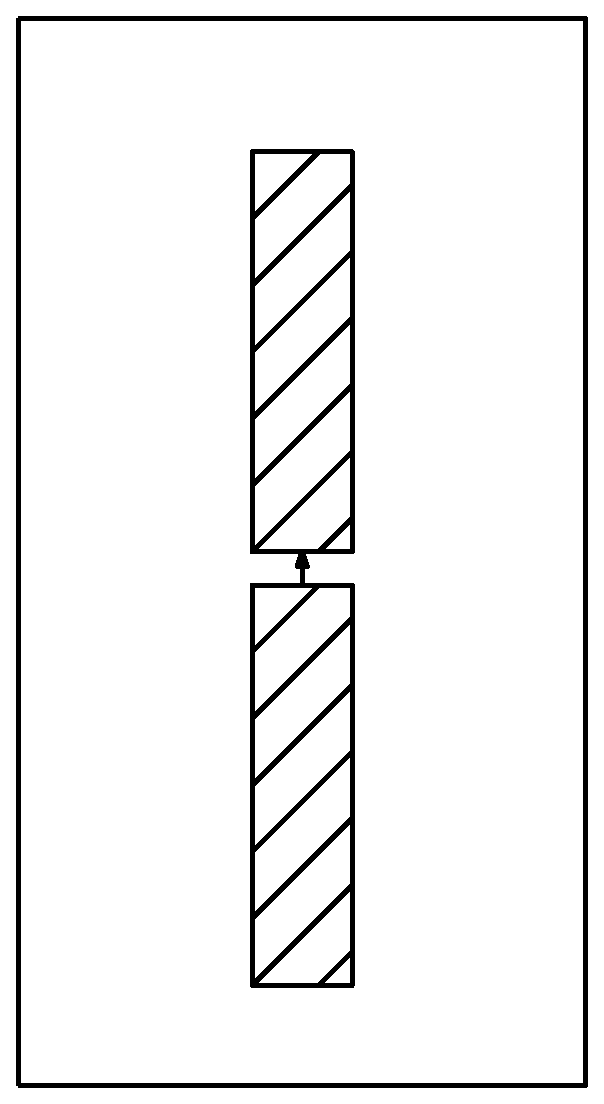
\includegraphics[scale=.5]{Figures/Chapter1/slow_waveguide_structure/a}} 
\hspace*{\fill}
\subfloat[]{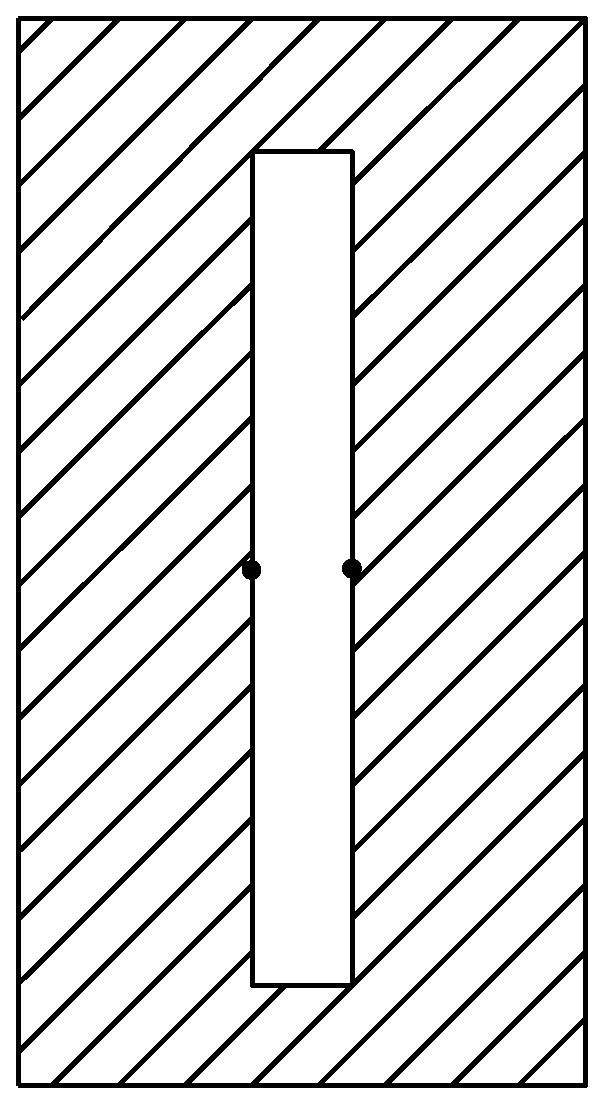
\includegraphics[scale=.5]{Figures/Chapter1/slow_waveguide_structure/b}} 
\hspace*{\fill}

\hspace*{\fill}
\subfloat[]{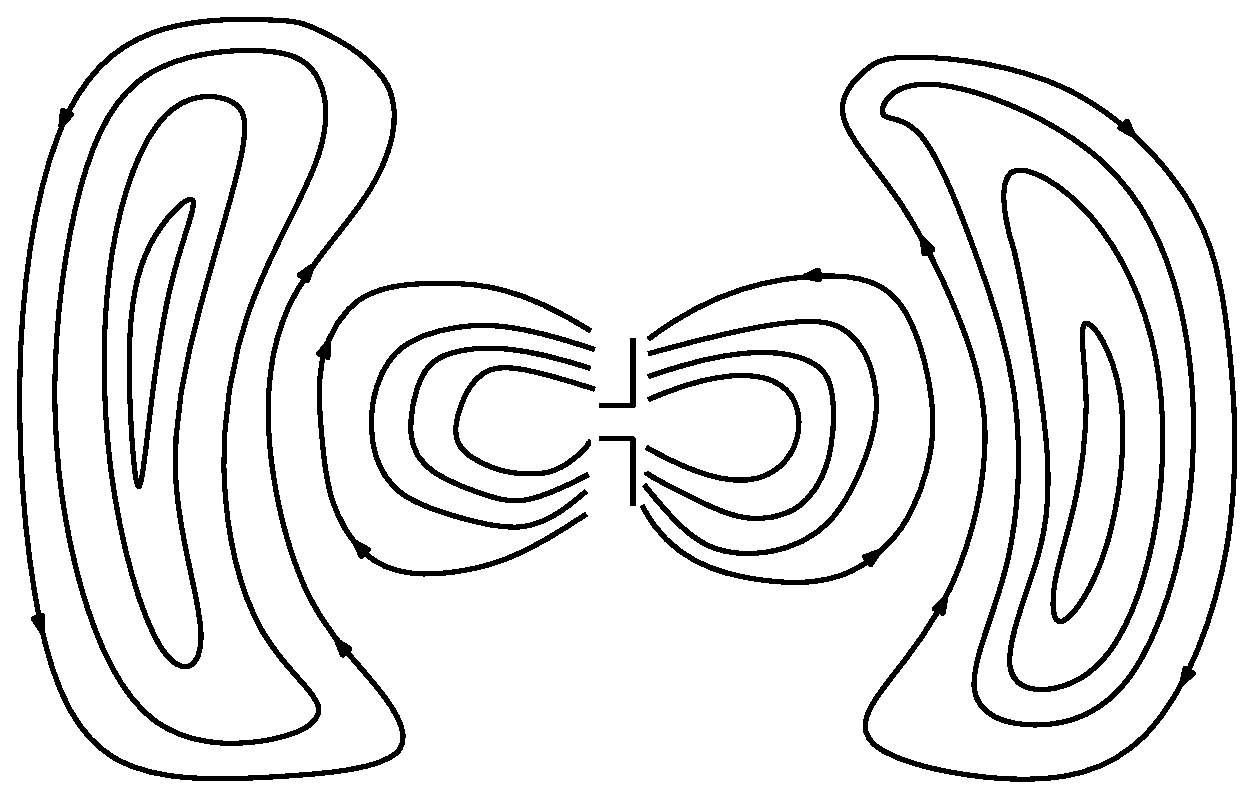
\includegraphics[scale=.5]{Figures/Chapter1/slow_waveguide_structure/c}}
\hspace*{\fill}
\subfloat[]{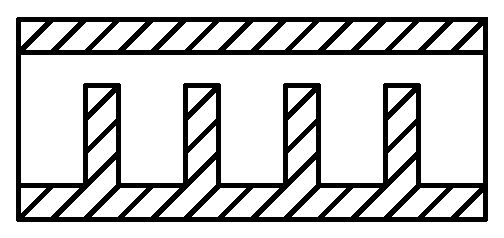
\includegraphics[scale=.5]{Figures/Chapter1/slow_waveguide_structure/d}} 
\hspace*{\fill}

\hspace*{\fill}
\subfloat[]{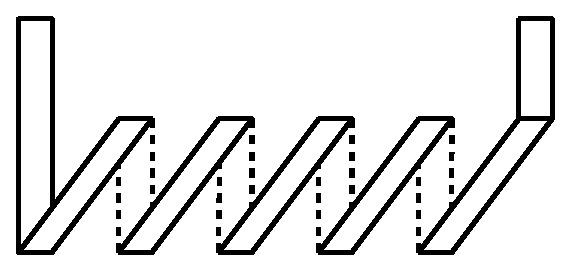
\includegraphics[scale=.5]{Figures/Chapter1/slow_waveguide_structure/e}} 
\hspace*{\fill}
  \caption[Models of simple slow-wave structures including folded-back transmission line, zigzag transmission line, interdigital transmission transmission line, corrugated transmission waveguide, and helix transmission line.]{Models of simple slow-wave structures. (a) Folded-back transmission line. (b) Zigzag transmission line. (c) Interdigital transmission transmission line. (d) Corrugated transmission waveguide. (e) Helix transmission line}
\label{fig:slowstrcture}
\end{figure}

The antenna proposed in the later chapters of this thesis is a leaky-wave antenna which utilizes fast waves as radiation mechanism. Therefore the following discussions are restricted to reviewing concepts of fast-wave radiation. 

%%%%%%%%%%%%%%%%%%%%%%%%%%%%%%%%%%%%%
\subsubsection{Fast-wave}
A fast wave has a phase velocity greater than the velocity of light in that medium ($v_p > \mathrm{c}$). Hence, the propagation constant of a fast wave is less than that of light as shown in the following equation
%
\begin{equation}
  \beta_{fast}= \dfrac{\omega}{v_p}  < k_0= \dfrac{\omega}{\mathrm{c}} 
\end{equation}
%
where $\omega $ is the operating frequency, $k_0$ and $\mathrm{c}$ is the wave constant and velocity of light in that medium, respectively. The fundamental $TE_{10}$ mode of a rectangular waveguide and higher order modes in a parallel plate waveguide are example of fast waves. A fast wave is capable of simultaneously \textit{leaking} energy into free-space \cite{Neto2010}\cite{felsen1994}.% Cherenkov radiation occurs when an electrically charged particle moves with higher phase velocity than the speed of light in the same medium . 

%
\begin{figure} [!t]
\centering
\noindent
\begin{overpic}[scale=0.8]{Figures/Chapter1/LWA_waveguide/LWA_waveguide}
		\put(51,40){\footnotesize $z$}
		\put(40,36){\footnotesize $y$}
		\put(97,19){\footnotesize $x$}
		\put(65,34){\footnotesize $\theta$}
		\put(94,28){\footnotesize Decay of}
		\put(94,25){\footnotesize LW mode}
		\put(-5,14){\footnotesize $\mathbf{E} = \hat{\mathbf{y}}e^{ - j \beta x}$}
    \put(70,37){\footnotesize $ \mathbf{E}(x,z) = \hat{\mathbf{y}}e^{ - j \beta x}e^{ - j \sqrt{k_0^2 - \beta^2} z}$}

\end{overpic}
\caption[Transition of a bounded wave from a rectangular waveguide to a structure that supports leaky-wave mode.]{Transition of a bounded wave from a rectangular waveguide to a structure that supports leaky-wave mode. A fast wave (dotted line with arrow-head) that propagates through a closed waveguide in the negative $x$ region remains trapped inside the structure. The grey region along the upper wall of the waveguide represents a slot aperture in the positive $x$ region. The propagating wave in this region is a leaky-wave mode that leaks energy through the longitudinal aperture of the structure. The propagating leaky-wave mode decays exponentially inside the waveguide.}
\label{fig:LWA_waveguide} 
\end{figure}
%
\subsubsection{Radiation from slow and fast waves}
To demonstrate how a propagating fast wave generates radiation, a guided structure located at $z<=0$ is considered in Fig. \ref{fig:LWA_waveguide}. The structure is surrounded by free space. The region in the positive-$x$ has a slot aperture along its upper wall in $xy$ plane. The aperture introduced along the length of the transmission line in positive-$x$ region allows the propagating wave to continuously leak its energy provided that the its propagation constant is $\beta_{fast}  < k_0$. The radiation in $z>0$ forms a conical beam. The normalized field distribution of the bound wave on the aperture is given by
%
\begin{equation} \label{eq:leaky-wave antenna1}
\mathbf{E} = \hat{\mathbf{y}}e^{ - j \beta x}
\end{equation}
%
where, $\hat{\mathbf{y}}$ is the direction of electric field, $\beta$ is the wave number of the wave propagating in the $x$ direction. The wave number $\beta$ depends on the type of bounded wave inside the guided structure. It equals to the free-space wave number $k_0$ if the structure line is a parallel-plate waveguide filled with air. In contrast, $\beta$ becomes larger (slow wave) than $k_0$ if the waveguide consists of dielectric materials. $\beta$ can also be smaller than $k_0$ (fast wave) for higher order modes of a parallel plate waveguide. The radiating mode from a wave having a phase velocity faster than that of light is known as leaky wave mode.

We are interested to study the radiation produced in the region $z>0$ by the planar aperture. We use the Fourier transform method demonstrated in \cite{Collin1985}, chapter 4. The solution for the electric field in free-space $(z>0)$ is expressed as
%
\begin{equation} \label{eq:leaky-wave antenna2}
    \mathbf{E}(x,z) = \hat{\mathbf{y}}e^{ - j \beta x}e^{ - j \sqrt{k_0^2 - \beta^2} z}
\end{equation}
%
Eq. \ref{eq:leaky-wave antenna2} states that if a wave defined by Eq. \ref{eq:leaky-wave antenna1} propagates along an infinitely long slot, the corresponding fields in free-space has both $x$ and $z$ components of propagation constant. If the propagating wave along the slot is slow $(\beta > k_0)$, the term $\sqrt{k_0^2 - \beta^2}$ becomes imaginary, which results in evanescent waves in the region $z<0$. In contrast, if the propagating wave along the slot is fast $(\beta < k_0)$, a plane wave is generated from the slot at an angle given by the following equation
\begin{equation} \label{eq:ktheta}
     \mathrm{sin}\theta = \dfrac{\beta}{k_0}
\end{equation}
The amplitude of the traveling-wave exponentially decays in the direction of propagation due to constant leakage of energy through the slot. The exponential decay of the wave is expressed by attenuation constant $\alpha$ which is related to the cross-sectional geometry of the transmission line. It is be noted that attenuation constant $\alpha$ of a leaky-wave mode is not necessarily related to the material loss, but can appear due to radiation losses alone. As for the propagation constant $\beta$ in Eq. \ref{eq:leaky-wave antenna1}, it represents the phase constant of the wave in the transmission line. $\beta$ determines the nature of the traveling-wave and the amplitude constant $\alpha$ is the leaked energy per unit length. Most of the characteristics of a leaky-wave antenna is governed by the two parameters $\alpha$ and $\beta$.

To account for the decay of the leaky-wave mode, a decreasing exponential term $e^{-\alpha x}$ is incorporated with the expression for the fields in Eq. \ref{eq:leaky-wave antenna1}. 
%
\begin{subequations} 
\begin{align}
\mathbf{E} &= \hat{\mathbf{y}}{e^{ - j\beta x}}{e^{-\alpha x}} \\
\mathbf{E} &= \hat{\mathbf{y}}{e^{ - j\beta x}}{e^{j^2\alpha x}} \\
\mathbf{E} &= \hat{\mathbf{y}}{e^{ - j(\beta  - j\alpha )z}} 
\end{align}
\end{subequations}
%
where, $\beta$ is the phase constant of the propagating wave prior to introducing the aperture and $\alpha$ is the leakage constant of the leaked power \cite{Jackson2008}. From the above equation, it can be concluded that the propagation constant of a leaky wave mode into free space is represented by
%
\begin{equation} \label{eq: klw}
   k_{\mathrm{LW}} = \beta  - {\rm{j}}\alpha 
\end{equation} 
%
\begin{figure} [t!]
\centering
\noindent
\begin{overpic}[scale=0.6]{Figures/Chapter1/linesource/linesource}
    \put(55,10){\footnotesize $L$}
    \put(47,18.5){\footnotesize $x$}
    \put(19,42){\footnotesize $z$}
     \put(25,36){\footnotesize $\theta$}

\end{overpic}

\caption{Line-source model of a leaky-wave structure.}
\label{fig:linesource}
\end{figure}

The fields created by a leaky wave mode described in Eq. \ref{eq:leaky-wave antenna1} corresponds to infinitely long apertures. Finding the fields in free-space for a finite aperture is more complicated \cite{Mahmoud2010}. The process can be simplified by replacing the finite aperture by a line-source model extended in the positive $x$ direction as demonstrated in Fig. \ref{fig:linesource}\cite{Stutzman2012}. With the line-source model, the leaky-wave structure can be assumed as a lossless waveguide with a uniform cross section that supports a traveling wave with a phase constant $\beta$ in the $x$ direction. Since leaky-wave radiates from a uniform cross-section, all leaky-wave antennas can be expressed by a line-source with a voltage distribution \cite{zelinski2005}:. 
\begin{equation}
V(x) = e^{-j \beta x}
\end{equation}
where $k_{\mathrm{LW}}$ is the complex leaky-wave number as expressed by Eq. \ref{eq: klw}.  The substitution facilitates a straightforward approach using scalar quantities like far-field radiation pattern \cite{Sutinjo2008}. The far field radiation pattern of the radiated wave is given by:
%
\begin{equation}
f(\theta) = \int_{0}^{L} e^{-jk_{\mathrm{LW}}x} e^{-jk_0 \sin\theta x} dx 
\end{equation} 
%
It is known the the integral of such format can be express in terms of a $sinc$ function:
%
\begin{equation} \label{eq:kff}
f(\theta) = \mathrm{sinc} \bigg[ (\beta - k_0 \sin\theta) \dfrac{L}{2}) \bigg] L 
\end{equation}
%
The peak of the radiation pattern $f(\theta)$ is evaluated at an angle $\theta_m$:
\begin{equation}
 \sin \theta_m = \dfrac{\beta}{k_0}
\end{equation}
which is the similar found in Eq. \ref{eq:ktheta} through field quantities.

Eq. \ref{eq:kff} can result in different kinds of radiation depending on the proporty of $\beta$. For a fast wave with $\beta < k_0$ the case is quite simple. The direction of radiation at an angle $\theta_m$ is given by the Eq. \ref{eq:ktheta}. As presented in Eq. \ref{eq:kff}, the far field function $f(\theta)$ is represented by $\mathrm{sinc}$ which is a continuous function. Therefore, the far field radiation pattern contains sidelobes. This is different from radiation pattern of an infinite structure which is free of sidelobes. All practical leaky-wave antennas have a finite structure and consist of sidelobes originated from reflected backward waves in the transmission line. %For $\beta=k_0$, the peak of the radiation angle is found as follows:
%\begin{equation}
%\theta_m = \mathrm{\arcsin} \dfrac{\beta}{k_0}= 90^o
%\end{equation}
%which indicates an endfire radiation.

A periodic leaky-wave antenna uses a slow wave as radiation mechanism. Equation \ref{eq:kff} suggest that for slow waves with $\beta>k_0$ leads to a complex value of radiation peak radiation angle  $\theta_m$ ($= \arcsin (\beta / k_0) > 1$). Therefore, if a slot-line is introduced to a slow-wave structure, radiation is not achieved in free-space. However, it was found that a propagating slow-wave can radiate if the associated aperture, rather than being longitudinally uniform, has periodic perturbations. Periodic modulations at the aperture introduces infinite number of space harmonics in the guided wave in the transmission line, provided that the main space harmonic is a slow wave \cite{Tamir1969}\cite{Hessel1969}. The perturbations are introduced in such a way that one of the space harmonics is a fast wave having a wave number less than $k_0$ \cite{Jackson2008}. Radiation is obtained through allowing the fast space harmonics to leak energy into free-space\cite{Sutinjo2008}. Such emission is known as \textit{slow leaky-wave radiation}.

\begin{figure} [t!]
\centering
\hspace*{\fill}%
	\mbox{\subfloat[]{
  \begin{overpic}[scale=0.6]{Figures/Chapter1/microstripLWA/microLWAa}
				\put(50,3){\footnotesize $\mathbf{E}$ plane}

	\end{overpic}}}
\hspace*{\fill}%

\hspace*{\fill}%
  \mbox{\subfloat[]{
  \begin{overpic}[scale=0.6]{Figures/Chapter1/microstripLWA/microLWAb}
			    \put(45,4){\footnotesize $\mathbf{E}$ plane}

	\end{overpic}}}
	  \hspace*{\fill}%
  \caption[Leaky-wave antennas based on microstrip structures including the comb line array and a series microstrip patch array.]{Leaky-wave antennas based on microstrip structures: (a) the comb line array and (b) series microstrip patch array \cite{Sutinjo2008} \textcopyright 2008 IEEE.}
\label{fig:microLWA}
\end{figure}

%Examples of uniform and periodic lekay-wave antenna structures are demonstrated is presented in section \ref{chap0:LWA}. The fundamental $TE_{10}$ mode of a rectangular waveguide, higher order modes in a parallel plate waveguide are example of fast waves. A rectangular waveguide with a uniform opening along the length is a popular example of uniform leaky-wave antenna. The phase velocity of the traveling wave inside the waveguide is given by
%\begin{equation} \label{eq:wg}
%{v_{phase}} = \dfrac{c}{{1 - \sqrt {{{\left( {\dfrac{c}{{2af}}} \right)}^2}} }}
%\end{equation}
%Where, $f$ is the operating frequency and $a$ is the width of the waveguide. Equation \ref{eq:wg} suggests that for the traveling wave, $ v_{phase}$ is greater than ${\rm{c}}$ (fast wave). Therefore, an aperture introduced on a rectangular waveguide couples leaky-wave radiation from the structure to the air.  In contrast to air-filled waveguide, a dielectric-filled one does not fundamentally radiate through a uniform aperture. However, introduction of the perturbations along the length causes it to generate slow leaky-wave radiation. Other examples of leaky-wave antenna that utilizes fundamentally slow wave to generate radiation include the microstrip comb line and series-fed patch microstrip arrays illustrated in Fig. \ref{fig:microLWA}a and \ref{fig:microLWA}b, respectively \cite{james1981}. A microstrip line supports slow TEM wave \cite{Menzel1979}. Phase velocity of the wave inside the microstrip line is given by
%
%\begin{equation}
  %  {{\rm{v}}_{phase}} = \dfrac{c}{{\sqrt {{\varepsilon _{eff}}} }}
%\end{equation}
%
%where, ${\varepsilon _{eff}}$ is the effective permittivity of dielectric inside the microstrip line. To make this fundamentally slow transmission line to radiate, periodic perturbations are required to be intorduced. The design of these arrays were not initially motivated to achieve leaky-wave radiation until suggested in \cite{Oliner2007} and later confirmed in \cite{Sutinjo2008}. 

%%%%%%%%%%%%%%%%%%%%%%%%%%%%%%%%%%%%%%%%%%%%%%%%%%%%%%%%%%%%%%%%%%%%%%%%%%%%%%%%%%%%%%%%%%%%%%%%%%%%%%%%%%%%%%%%%%%%%%%

\subsection{Radiation characteristics} 

\subsubsection{Direction of primary beam}
 \begin{figure}[t]
	\centering
 	\noindent

  \begin{overpic}[scale=0.6]{Figures/Chapter1/LWA_performance/LWA_beamdirection}
   \put(60,3.5){\footnotesize LWA guiding structure}
   \put(97,5){\footnotesize $x$}
   \put(-2,5){\footnotesize $-x$}
   \put(52,48){\footnotesize $z$}
   \put(57,28){\footnotesize $\theta$}
   \put(75,30){\footnotesize Forward quadrant}
   \put(0,30){\footnotesize Backward quadrant}
   \put(90,10){\footnotesize Endfire}
   \put(35,50){\footnotesize Broadside}
   \put(15,45){\footnotesize Frequency increase}
  \end{overpic}
 	\caption[Beam-scanning performance of a typical leaky-wave antenna.]{Beam-scanning performance of a typical leaky-wave antenna. The primary beam scans the space from backward quadrant (only for periodic structures) to forward quadrant (for periodic and uniform structures).}
 	\label{fig:LWscan}
 \end{figure}
The radiated beam from a leaky-wave antenna has a conical shape. The direction of maximum radiation is obtained from equation  \ref{eq:ktheta} is expressed as
%
\begin{subequations} 
\begin{align}
    \theta &= \arcsin \dfrac{\beta}{k_0} \\ \label{eq:thetam12}
           &= \arcsin \dfrac{\lambda_0 }{\lambda_g} \\ 
           &= \arcsin \dfrac{c}{v_{\mathrm{LW}}} \label{eq:thetam1}
\end{align}
\end{subequations}
%
where $\lambda_0$ and $\mathrm{c}$ is the free-space wavelength and velocity of the radiated wave, $\lambda_g$ and $v_{LW}$ is the wavelength and phase-velocity of leaky-wave mode inside the guiding structure and $\theta$ is the direction of maximum radiation measured from broadside direction. Equation \ref{eq:thetam1} shows that the angle of radiation from a leaky-wave antenna depends on free-space wavelength $\lambda_0$, hence on operating frequency. As the operating frequency is increased, the angle of peak radiation $\theta$ increases from broadside towards endfire. The beam-scanning performance as well as the regions of radiation is demonstrated in Fig. \ref{fig:LWscan}. Uniform leaky-wave antennas can only operate in the forward quadrant. On the other hand, periodic leaky-wave antennas offer the flexibility to obtain radiation both in forward and backward quadrants. It is generally difficult to obtain radiation near endfire region ($\theta = 90^o$) for an air-filled waveguide. The scanning operation near endfire requires the antenna to operate at frequencies above cutoff of the leaky-wave mode. 

%%%%%%%%%%%%%%%%%%%%%%%%%%%%%%%%%

\subsubsection{Beam-width}
 \begin{figure}[t]
	\centering
 	\noindent
 	{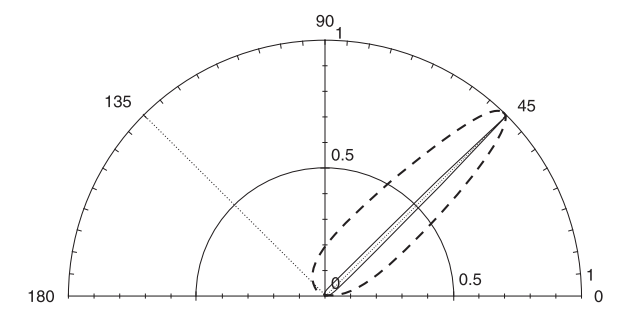
\includegraphics[scale=.6, keepaspectratio=true]{Figures/Chapter1/LWA_performance/beamwidth.PNG}}
 	\caption[Radiation patterns showing the variation of beamwidth with the change of leakage constant of a leaky-wave antenna.]{Radiation patterns for a leaky mode having $\beta/k_0=0.7071$ and two different values of $\alpha/k_0:0.1$ (dashed line) and $0.01$ (solid line) \cite{Jackson2008}.}
 	\label{fig:fixedBW}
 \end{figure}

Another interesting feature of leaky-wave antenna is that the beamwidth (between the $-3$dB points) of the main lobe varies very little with the variation of frequency. While the beam direction in Eq. \ref{eq:thetam1} depends on $\beta$, beamwidth is controlled by the attenuation constant $\alpha$. The beamwidth for uniform leaky-wave antenna is given by the following equation \cite{Jackson2008}:
%
\begin{equation}\label{eq:deltheta}
  \Delta \theta  \approx \dfrac{1}{{\dfrac{L}{{{\lambda _0}}}\cos {\theta _m}}}  \propto \dfrac{\dfrac{\alpha}{k_0}}{\cos {\theta _m}}
\end{equation}
%
where $\Delta \theta$ is the beamwidth, $\theta _m$ direction of maximum radiation and $L$ is the length of the aperture of the leaky-wave antenna. It is to be noted that the angle of radiation $\theta_m$ is dependent on frequency as shown in Eq. \ref{eq:thetam1}. However, the beamwidth $\Delta \theta$ depends on the length of the aperture $L$ in terms of wavelength $\lambda_0$. A large value of $\alpha$ indicates a short effective aperture, leading to a large beamwidth of the radiated wave. On the other hand, smaller value of $\alpha$ leads to a longer effective aperture of the antenna structure, making the beam narrower. Radiation patterns in the scanning plane for two values of $\alpha/k_0$ are presented in Fig. \ref{fig:fixedBW} \cite{Jackson2008} where radiation is achieved at an angle $\theta _m = 45^o$. In accordance with Eq. \ref{eq:deltheta}, the pattern having larger $\alpha$ value has a much larger beamwidth. Note that the radiation patterns in Fig. \ref{fig:fixedBW} do not have side-lobes because they correspond to an infinite uniform leaky-wave antenna.

Equations \ref{eq:thetam1} and \ref{eq:deltheta} suggests that as frequency is increased in a leaky-wave antenna, the main beam steers from broadside towards endfire while maintaining a constant beamwidth.

 
% \begin{figure}[!htp]
 %	\centering
% 	\noindent
 %	\subfloat[Linear Phase  \label{fig1:leaky-wave antenna}]{\includegraphics[trim={0cm 0cm 0cm 0cm},clip,scale=.6, %keepaspectratio=true]{Figures/Chapter1/leaky-wave antenna.pdf}}
 %	\caption{Leaky-wave antenna.}
% 	\label{fig:leaky-wave antenna}
 %\end{figure}


%%%%%%%%%%%%%%%%%%%%%%%%%%%%%%%%%%%%%%%%%%%%%%%%%%%%%%%%%%%%%%%%%%%%%%%%%%%%%%%%%%%%%%%%%%%%%%%%%%%%%%%%%%%%%%%%%%%%%
\section{Slot-line leaky-wave antenna} \label{sec:slotLW}

\subsection{Principle of radiation} \label{SLLWA}
 
\begin{figure} [t]
\centering
\noindent
\hspace*{\fill}%
	\mbox{\subfloat[]{
  \begin{overpic}[scale=0.35]{Figures/Chapter1/complementary/a}
				\put(10,22){\footnotesize Air }
				\put(15,46){\footnotesize I }

	\end{overpic}}}
	%
\hspace*{\fill}%
%
	\mbox{\subfloat[]{
  \begin{overpic}[scale=0.35]{Figures/Chapter1/complementary/b}
  
        \put(24.5,46){\footnotesize V }

	\end{overpic}}}
  \hspace*{\fill}%  
\caption[Complementary electric dipole in free-space and slot-line on an infinite conductive plane.]{Complementary electric dipole in free-space excited with a current $I$ (a) and slot-line on an infinite conductive plane excited with a current $V$ (b).}
\label{fig:complementary}
\end{figure} 

A slot-line on an infinite conductive plane and an electric dipole in free-space are complementary structures \cite{Kong1990}. Illustrated in Fig. \ref{fig:complementary}, antenna A is the complementary structure of antenna B. The shaded region in Fig. \ref{fig:complementary}b is an infinite ground plane. The field radiation from an electric dipole is calculated using electric currents since it radiates using electric currents. In contrast, field calculation for a slot antennas can also be done by considering nearby surface currents. However, evaluation of slot radiation becomes simpler if the source of radiation is considered to be a fictitious magnetic current. %The analysis is done by replacing the loop current by small magnetic dipoles, similar to electric dipoles. 
%
Using full-wave analytic techniques, existence of leaky-wave mode on a transversely excited slot-line was first reported in 1988 \cite{Shigesawa1988}. Following a similar approach, Neto and Maci analyzed the magnetic currents of an infinitely long slot-line placed between two homogeneous media in 2003 \cite{Neto2003}\cite{Maci2004}. The fictitious magnetic current corresponding to the slot aperture was analyzed in order to obtain and solve the dispersion relation of the slot mode. 
%
\begin{figure} [t]
\centering
\noindent
\begin{overpic}[scale=0.5]{Figures/Chapter2/fig_singleslot/singleslot}
		\put(42,38){\footnotesize Ground plane}
		\put(38,25){\footnotesize Dielectric }
		\put(35,20){\footnotesize half-space $(\epsilon_{r1})$}
		\put(33,80){\footnotesize Dielectric }
		\put(30,75){\footnotesize half-space $(\epsilon_{r2})$}
		\put(50,68){\footnotesize $z$}
		\put(90,47){\footnotesize $x$}
		\put(34,55){\footnotesize $y$}

\end{overpic}
\caption[Infinitely stretched slot located at the interface of two dielectric half spaces.]{Infinitely stretched slot located at the interface of two dielectric half spaces. The slot is etched on a ground plane \cite{Neto2003} \textcopyright 2003 IEEE.}
\label{fig:singleslot} 
\end{figure}
%
The electric dipole source excitation was expanded in the spectral domain, followed by solving the dispersion equation of the slot-line using Fourier transform. The detailed analytical expressions are beyond the scope of this thesis. In order to explain the steps in brief, an infinite slot etched in a perfect electric conductor (PEC) ground plane is illustrated in Fig. \ref{fig:singleslot}. The slot is excited by a transverse current element in $y$ direction. The upper half $(z>0)$ and lower half $(z<0)$ of the slot consist of homogeneous dielectrics while with a relative dielectric permittivity $\epsilon_{r1}$ and $\epsilon_{r2}$, respectively. The normalized magnetic current (voltage) along the slot in spectral domain is expressed as \cite{Neto2003}:

\begin{equation} \label{magcurspec}
V(k_x) = - \dfrac{2\pi}{\int_{-\infty}^{\infty} G(k_x, k_y) J_0 ( \dfrac{1}{2} w_s k_y ) d k_y} 
\end{equation}
where, $J_0$ is the Bessel function of zero order, $w_s$ is the thickness of the slot, $G(k_x, k_y)$ is the Fourier transform of Green's function of a slot placed in between two dielectric half spaces is given by 
\begin{equation} \label{slotgreen}
 G(k_x, k_y) = - \dfrac{1}{k_0 \zeta_0} \sum_{i=1}^{2} \dfrac{k_i^2 - k_x^2}{\sqrt{k_i^2 - k_x^2 - k_y^2}}
\end{equation}
where $k_0$ is the free-space propagation constant, $\zeta_0$ is the characteristic impedance, and $k_i$ for $i=1,2$ are the wave numbers in medium 1 and 2 respectively. By applying the Green's function from Eq. \ref{slotgreen} in Eq. \ref{magcurspec}, the normalized voltage along the slot-line can be obtained by applying inverse-Fourier transformation:
\begin{equation} \label{magcur}
    v(x) = \dfrac{1}{2 \pi} \int_{-\infty}^{\infty}  e^{-j k_x x} V(k_x) d k_x
\end{equation}
%
\begin{figure} [t]
\centering
\noindent
\begin{overpic}[scale=0.4]{Figures/Chapter2/fig_singleslot/lswave}
%\put(55,83){\footnotesize $\theta$ }
%\put(15,60){\footnotesize $\epsilon_{r2}$ }
%\put(15,30){\footnotesize $\epsilon_{r1}$ }
\end{overpic}
%


\caption[A radiation pattern comparing the leaky-wave and source wave radiation originating from a slot-line.]{(color inline) A sketch of a radiation pattern showing that the slot-emitted leaky wave (blue) radiates predominantly into the denser (upper) dielectric half-space. Two beams are generated since the slot-line is excited in the center. The spherical source wave (red) is competitively weaker in power.}
\label{fig:lswave} 
\end{figure}

The complex propagation constant of the leaky wave mode along the slot can be obtained by solving Eq. \ref{magcur} \cite{Neto2005}. If the upper dielectric half-space has higher dielectric permittivity than the one at the bottom ($\epsilon_{r2} > \epsilon_{r1}$), the complex propagation constant $k_x^{\mathrm{LW}}$ is given by the following equation
%
\begin{equation} \label{eq:kslot}
	k_x^{\mathrm{LW}} \approx \beta  + \dfrac{{k_d^2}}{{2\beta \left[ {1 - j\dfrac{4}{\pi }\ln \left( {\gamma_e {k_d}\dfrac{w_s}{8}} \right)} \right]}} 
\end{equation}
%
where, ${\gamma_e=\exp(\gamma)=1.781\ldots}$ is the exponential of Euler constant, $\beta$ and $k_d$, associated with the average permittivity of media 1 and 2, is expressed as 
%
\begin{subequations}
	\begin{align}
		\beta &=   \dfrac{\sqrt{k_1^2+k_1^2}} {2} \\
		k_d & =  \dfrac{\sqrt{k_2^2-k_1^2}} {2} 
	\end{align}
\end{subequations}
%
provided that medium 2 is the denser medium. Equation \ref{eq:kslot} suggests that if the width of the slot $w_s$ is very narrow, then the propagation constant of the fast wave mode along the slot ($k_x^{\mathrm{LW}} $) simplifies to be:
%
\begin{equation} \label{eq: kslotsimple}
	k_x^{\mathrm{LW}} = \beta  =  \dfrac{\sqrt{k_1^2+k_1^2}}{2} 
\end{equation}
%
which is an established expression stating the slot-line mode has a phase constant between that of the associated medium \cite{Galejs1962}.

The propagating leaky-wave mode is fast for the upper dielectric region and slow for the lower halfspace. Therefore, the slot generates leaky-wave radiation into the upper dielectric halfspace. Radiation in the denser media is obtained from Eq. \ref{eq:thetam12}:
\begin{equation} \label{eq:thetam123}
	\theta = \arcsin \dfrac{k_x^{\mathrm{LW}}}{k_2}
\end{equation}
where $k_x^{\mathrm{LW}}$ and $k_2$ is the wave number of the leaky-wave mode and radiated wave, respectively (see Fig. \ref{fig:lswave}). Equation \ref{eq:thetam123} can be simplified by applying the relation of Eq. \ref{eq: kslotsimple} as below:
%
\begin{subequations} 
	\begin{align}
		\theta & = \arcsin \dfrac{k_x^{\mathrm{LW}}}{k_2} \\
		& = \arcsin \dfrac{\dfrac{\sqrt{k_1^2+k_1^2}}{2}}{k_2} \\
		& = \arcsin \dfrac{\sqrt {\epsilon_{r1} + \epsilon_{r2}}}{2 \epsilon_{r2}} \label{eq:slottheta}
	\end{align}
\end{subequations}
where, ${\theta}$ is measured from the broadside. The direction of radiation in Fig. \ref{fig:lswave} is independent of frequency since it is a function of the permittivity values of the associated media. This implies that the leaky-wave mode in the slot produces a beam which is directed at a fixed angle irrespective of frequency. Apart from the leaky-wave radiation, the slot generates a spherical source wave from the excitation \cite{Maci2004}. The source wave contributes to the fields in the upper dielectric half-space; however, is weak when the slot is narrow in terms of wave length. Therefore it does not affect the fixed-beam performance and wide input impedance bandwidth of the slot. The polar plot in Fig. \ref{fig:lswave}  shows the leaky-wave (blue line) and spherical source wave radiation (red line) pattern originating from a  center-fed leaky-wave antenna.


%%%%%%%%%%%%%%%%%%%%%%%%%%%%%%%%%%%%%%%%%%%%%%%%%%%%%%%%%%%%%%%%%

\subsection{Fixed-beam leaky-wave antennas}

The leaky-wave radiation emitted from a slot placed at the interface of two different dielectric media can be utilized to design a fixed-beam leaky-wave antenna. There are three major designs available in the literature that involve fixed-beam leaky-wave radiation. The design principles and radiation mechanism of these antennas are described in this section.

\subsubsection{Dielectric lens}
Neto \textit{et al.} designed and built the first fixed-beam leaky-wave antenna utilizing the slot-generated leaky-wave radiation \cite{Neto2005}. The actual structure of the antenna is presented in Fig. \ref{fig:elliptical}. The design consisted of a dielectric half circle placed on top of a slot-line printed on a ground plane. The dielectric permittivity of the free-space region below the slot is lower than that of the dielectric lens. The slot-line generates leaky-wave radiation into the elliptical lens. The outer surface of the lens couples the radiation into free-space, resulting in broadside radiation. The antenna operated with a percentage bandwidth of $43\%$ ($-13$ dB $S_{11}$) and was later improved to $160\%$ ($-8.5$ dB $S_{11}$) \cite{Bruni2007} and $173\%$ \cite{Neto2010_2}. However, the overall antenna structure was electrically large. 

\begin{figure} [t!]
\centering
\noindent
\hspace*{\fill}%
	\mbox{\subfloat[]{
\begin{overpic}[scale=0.79]{Figures/Chapter1/elliptical/neto_reallens}
\end{overpic}}}
%
\hspace*{\fill}%
%
\mbox{\subfloat[]{
\begin{overpic}[trim={0cm 0cm 0cm 1.0cm},clip, scale=0.6]{Figures/Chapter1/elliptical/elliptical}
\put(10,23){\footnotesize $\epsilon_r>1$ }
\end{overpic}
\hspace*{\fill}}}%

\caption[The prototype of Neto's fixed-beam leaky-wave lens antenna and a diagram demonstrating its radiation towards broadside.]{The prototype of Neto's fixed-beam leaky-wave lens antenna \cite{Neto2010_2} \textcopyright 2010 IEEE. The dielectric lens is the white hemispherical medium (a). Cross-section of the elliptical dielectric hemisphere placed of top of a leaky-slot. The gray region illustrates the dielectric lens with a permittivity $\epsilon>\epsilon_0$. The slot is represented by the gap between ground plane at the bottom of the lens (b).}
\label{fig:elliptical} 
\end{figure}

\subsubsection{Active non-Foster circuits}
The previous design involved a dielectric lens with permittivity $\epsilon>\epsilon_0$ that coupled leaky-wave radiation into free-space. As an alternative, coupling into free-space can be achieved if the slot is located on top of a substrate with a permittivity $0<\epsilon<\epsilon_0$. In that case, air would be denser as compared to the lower permittivity dielectric substrate. Therefore, the leaky-wave radiation would directly radiate into free-space from the slot. The substrate with relative permittivity ($\epsilon_r$) below unity can be implemented through metamaterials. Metamaterials are artificially produced materials that exhibits unusual properties not found in nature. Metamaterials offer a broad range of flexibility on engineering a medium that requires exotic values of constitutive parameters ($\epsilon$ and $\mu$). However, their resonant nature limits bandwidth of operation of the antenna \cite{Enoch2002}\cite{Garcia2002}. In contrast, active structures, achievable through non-Foster circuit elements, can be used for broadband applications. Sievenpiper proposed a structure for a microstrip line using such motivation and achieved fixed-beam leaky-wave radiation over a broad bandwidth \cite{Sievenpiper2011}. The design is presented in Fig. \ref{fig:nonfoster}. Although the structure was electrically long ($10\lambda_0$), it had comparatively small thickness ($.05\lambda_0$ at the highest operating frequency). The structure operated with a percentage bandwidth of $163.64\%$. Similar fixed-beam leaky-wave antennas with a substrate having a permittivity below $1$ has been studied in \cite{Mirzaei2015} and \cite{Long2014}.
%
\begin{figure} [t!]
\centering
\noindent
\begin{overpic}[scale=0.4]{Figures/Chapter1/elliptical/nonfoster}
\put(7,13){\footnotesize \rotatebox{-18}{$0<\epsilon_r<1$}}
\put(71,70){\footnotesize Microstrip line}
\end{overpic}
\caption{Diagram of a microstrip line with a superluminal substrate that is capable to radiate leaky-wave radiation into free-space.}
\label{fig:nonfoster} 
\end{figure}

\subsubsection{Metamaterial transition layer}
In 2014, Markley \textit{et al.} utilized transformation electromagnetics to propose a design of fixed-beam leaky-wave antenna \cite{Markley2014}. The antenna radiated using slot-line leaky-wave mode and consisted of a rectangular superstrate to couple the slot-generated radiation into free-space. 

\begin{figure} [t]
\centering
\noindent
\hspace*{\fill}%
	\mbox{\subfloat[]{
  \begin{overpic}[scale=0.35]{Figures/Chapter2/fig_metaprism/metaprism_a}
				\put(10,22){\footnotesize $\theta$ }

	\end{overpic}}}
	%
\hspace*{\fill}%
%
	\mbox{\subfloat[]{
  \begin{overpic}[scale=0.35]{Figures/Chapter2/fig_metaprism/metaprism_b}
  
        \put(30,65){\footnotesize $\theta_{rad}$ }

	\end{overpic}}}
  \hspace*{\fill}%  
\caption[Illustrations of slot-line leaky-wave antenna consisting of uniform dielectric prism and anisotropic inhomogeneous metamaterial tranistion layers.]{A slot-line leaky-wave antenna with a uniform dielectric prism layer (a) and an anisotropic inhomogeneous metamaterial layer (b).}
\label{fig:metaprism}
\end{figure}

The design principle is demonstrated in Fig. \ref{fig:metaprism}. A uniform dielectric prism in Fig. \ref{fig:metaprism} coupled the radiation into free-space. Using transformation electromagnetics, the prism was transformed into a rectangular transition layer as shown in Fig. \ref{fig:metaprism}. Figure \ref{fig:loic} shows full wave simulation of an anisotropic metamaterial transition layer designed using transformation electromagnetics which is placed on top of a slot. The superstrate couples the leaky-wave mode into free-space at a desired direction. 

The design technique offered flexibility in achieving a suitable radiation angle from the antenna. However, it lead to very high values of dielectric permittivity inside the superstrate. The transition layer presented in Fig. \ref{fig:loic} resembles a matched medium with equal permittivity and permeability values. The magnetic response of the anisotropic can be implemented using resonant metamaterials, which leads to narrow bandwidth of the antenna. %\textcolor{red}{An alternative design technique proposed alongwith incorporated anisotropic metamaterials which suffers from narrowband performance.}
\begin{figure} [t!]
\centering
\noindent
\begin{overpic}[scale=0.55]{Figures/Chapter2/fig_metaprism/loic.png}

\end{overpic}
\caption[Full-wave 2D simulations of the leaky-wave mode radiating into a metamaterial slab designed to couple to free-space.]{(color inline) Full-wave 2D simulations of the traveling-wave mode radiating into a metamaterial slab designed to couple to free-space \cite{Markley2014} \textcopyright 2014 IEEE.}
\label{fig:loic} 
\end{figure}


%%%%%%%%%%%%%%%%%%%%%%%%%%%%%%%%%%%

%The purpose of the rectangular superstrate in the target domain is to imitate the hemispherical medium in the source domain and produce identical radiation pattern into free-space.
% The principal component of the leaky-wave antenna, the inhomogeneous rectangular superstrate, is designed using transformation electromagnetics to serve as a transition layer that couples the leaky-wave radiation into free-space. It is optically transformed to behave like a hemispherical uniform dielectric medium.


%%%%%%%%%%%%%%%%%%%%%%%%%%%%%%%%%%%%%%%%%%%%%%%%%%%%%%%%%%%%%%%%%%%%%%%%%%%%%%%
\section{Transformation electromagnetics} \label{sec:TO}

Transformation electromagnetics is a method of manipulating electromagnetic fields through coordinate transformation. Although the idea behind transformation optics can be dated back to 1920s \cite{gordon1923}\cite{dyson1920}, it was not until 2006 when it received great attention \cite{Pendry2006}\cite{Leonhardt2009}. Transformation optics has been widely used as a convenient tool to design novel devices such as cloaks, super lenses \cite{Pendry2000} and antennas \cite{Leonhardt2008, Lier2011, Luo2009, Popa2009, Schmiele2010, Tichit2009}.

\subsection{Form invariance property of Maxwell's equations}
The transformation electromagnetics procedure is rooted in the form invariance of Maxwell's equations. The property allows them to stay in the same form under coordinate transformations. Ward and Pendry studied the propagation of electromagnetic waves in a complex structure defined by coordinate transformation \cite{Ward1996}. The frequency domain source free Maxwell's equations are presented in equations \ref{eq:subeq1}$-$\ref{eq:subeq4} which describes how electric and magnetic fields behaves in a linear isotropic dielectric media. 

Consider a coordinate transformation from the coordinate system ${(x,y,z)}$ to ${(x', y', z')}$. The transformed medium parameters are related by a Jacobian matrix which defines the coordinate transformation. It can shown that  equations \ref{eq:subeq1}$-$\ref{eq:subeq4} stay in the same form even if they are transferred from one set of coordinate system into another \cite{ozgun2010}. The transformed space would then be characterised by material parameters $\epsilon'$ and $\mu'$, electric field $\textbf{E}'$, magnetic field $\textbf{B}'$. Maxwells' equations in the transformed space can be expressed in the following form:
%
\begin{subequations}
	\begin{align}
		\mathbf{\nabla} \cdot \mathbf{B'}    = 0 \label{eq:subeq11}\\ 
		\mathbf{\nabla} \cdot \mathbf{D'}    = 0 \label{eq:subeq12}\\
		\mathbf{\nabla} \times \mathbf{E'} + j \omega \mu \mathbf{H'} = 0 \label{eq:subeq13}\\
		\mathbf{\nabla} \times \mathbf{H'} - j \omega \epsilon \mathbf{E'} = 0 \label{eq:subeq14}
	\end{align} 
\end{subequations}
%
Generally, the  material parameters ($\epsilon'$ and $\mu'$)  in the transformed medium coordinate system turn out as tensors, typically leading to non-isotropic and inhomogeneous medium. %These inherent properties enables light to bend inside the medium, creating exotic effects. 
%%%%%%%%%%%%%%%%%%%%%%%%%%%%%%%%%%%%%%%%%%%%%%%%%%%%%%%%%%%%%
\subsection{Conformal mappings in transformation optics}
\subsubsection{Coordinate mapping}
Conformal transformation maps a coordinate system into another without varying the local angles of the coordinate grid intersections. Consider the region $\mathrm{w}$ in Fig. \ref{fig:coordinatemapping}a defined by the coordinate system $(x$,$y)$ to be mapped into the region $\mathrm{t}$ in Fig. \ref{fig:coordinatemapping}b described by the coordinate system  $(u$,$v)$. The relation between the coordinate systems of the two regions is then given by 
\begin{equation} \label{eq:transformationrelation}
	(x,y) \overset{\mathrm{f}}{\longrightarrow} (u,v) 
\end{equation}


\begin{figure} [t]
	\centering
	\noindent
	\hspace*{\fill}%    
	\subfloat[Region $\mathrm{w}$ \label{subfig1:domain1}]{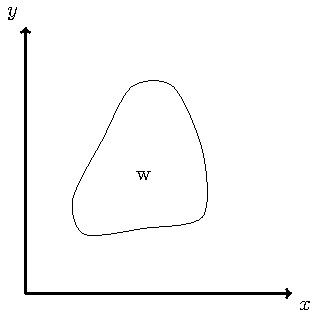
\includegraphics[trim={0cm 0cm 0cm 0cm},clip,scale=.9, keepaspectratio=true]{Figures/Chapter2/1a}}
	\hspace*{\fill}%
	\qquad
	\subfloat[Region $\mathrm{t}$   \label{subfig2:domain2}]{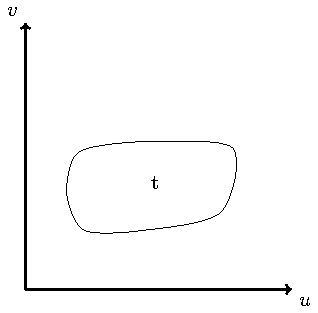
\includegraphics[trim={0cm 0cm 0cm 0cm},clip,scale=.9, keepaspectratio=true]{Figures/Chapter2/1b}}
	\hspace*{\fill}%  
	\caption[Coordinate mapping of region $\mathrm{w} = f(x,y)$ into a region $t = f(u,v)$.]{Coordinate mapping of region $\mathrm{w}$ in the $xy$ plane into a region $\mathrm{t}$ in $uv$ plane.}
	\label{fig:coordinatemapping}
\end{figure}

If $\mathrm{w}(x$,$y)$ is analytic (complex differentiable at every point) everywhere inside the domain, then $u$ and $v$ must satisfy the Cauchy-Reinmann conditions in equations \ref{eq:CR}a and \ref{eq:CR}b \cite{Saks1952}, for the mapping ($\mathrm{f}$) to be a conformal.
\begin{subequations} \label{eq:CR}
	%
	
	\begin{align}
		\dfrac{\partial u}{\partial x} &= \dfrac{\partial v}{\partial y}\\
		\dfrac{\partial u}{\partial y} &= -\dfrac{\partial v}{\partial x}
	\end{align} 
	%
\end{subequations}

Applying partial differentiation to the equations above with respect to $x$ and $y$ and relating the resulting equation, following relationships are obtained:
\begin{subequations} \label{eq:laplace}
	\begin{equation}
		\dfrac{\partial^2 u}{\partial x^2} + \dfrac{\partial^2 u}{\partial y^2} = 0
	\end{equation} 
	\begin{equation}
		\dfrac{\partial^2 v}{\partial x^2} + \dfrac{\partial^2 v}{\partial y^2} = 0
	\end{equation} 
\end{subequations}
Equations \ref{eq:laplace}a and \ref{eq:laplace}b are equivalent to Laplace's equations for analytic functions of $x(u,v)$ and $y(u,v)$. %This short derivation proves that all analytic function satisfies Laplace's equation.
%
%%%%%%%%%%%%%%%%%%%%%%%%%%%%%%%%%%%%%%%%%%%%%%%%%%%%%%%%%%%%%%%%%
\subsubsection{Local orthogonality}
It can be shown that if a conformal mapping is executed by satisfying Laplace's equation, the intersection angles of the $u$ and $v$ curves in region $\mathrm{t}$ would be the same as that of $x$ and $y$ curves in region $\mathrm{w}$ \cite{nehari1952}. In other words, conformal transformation preserves the local angles and aspect ratio between the intersecting grids. To demonstrate the local orthogonality, consider region $\mathrm{w}$ as the simplest orthogonal coordinate system: the Cartesian system, as demonstrated in Fig. \ref{fig:conformal}. 

\begin{figure}[t]
	
	\begin{center}
		
		\begin{overpic}[scale=.8]{Figures/Chapter2/conformal}
			\put(67,27){\footnotesize $\overrightarrow{dv}$}
			\put(75,20){\footnotesize $\overrightarrow{du}$}
			\put(12,15){\footnotesize $\overrightarrow{dx}$}
			\put(4,25){\footnotesize $\overrightarrow{dy}$}
			\put(10,-5){\footnotesize region $w(x,y)$}
			\put(70,-5){\footnotesize region $t(u,v)$}
		\end{overpic}
	\end{center} 
	
	\caption[Coordinate grid lines of constant $x$ and $y$ when conformally mapped from region $\mathrm{w}$ to region $\mathrm{t}$.]{Demonstration of conformal transformation. Coordinate grid lines of constant $x$ and $y$ is shown in domains $\mathrm{w}(x$,$y)$ and $\mathrm{t}(u$,$v)$.}
	\label{fig:conformal}
\end{figure}

As demonstrated in Fig. \ref{fig:conformal}, the coordinate lines of the region $\mathrm{w}(x$,$y)$ form a rectangular grid, intersecting orthogonally. There would always be a set of $u(x,y)$ and $v(x,y)$ curves that is constant for certain values of $x$ and $y$. Since $u(x,y)$ is constant in region $\mathrm{t}$, the differential $du$ would be zero. 
\begin{subequations} \label{eq:uconst}
	%
	\begin{equation}
		du = 0 
	\end{equation}  
	from the chain rule, 
	\begin{equation}
		\dfrac{\partial u}{\partial x} dx + \dfrac{\partial u}{\partial y} dy = 0 
	\end{equation}
	or,
	\begin{equation}
		\dfrac{\partial u}{\partial x} dx = - \dfrac{\partial u}{\partial y} dy 
	\end{equation}
	therefore,
	\begin{equation}
		\dfrac{dy}{dx}|_{u=\mathrm{constant}} = - \dfrac{\dfrac{\partial u}{\partial x}}{\dfrac{\partial u}{\partial y}}
	\end{equation}
	%
\end{subequations}
%
A similar relationship can be obtained for the constant $v(x,y)$ curves in region $\mathrm{t}(u$,$v)$:
\begin{equation} \label{eq:vconst}
	\dfrac{dy}{dx}|_{v=\mathrm{constant}} = - \dfrac{\dfrac{\partial v}{\partial x}}{\dfrac{\partial v}{\partial y}}
\end{equation}
Taking the product of equations \ref{eq:uconst}d and \ref{eq:vconst} and applying the Cauchy-Reinmann condition in Eq. \ref{eq:CR}:
%
\begin{equation} \label{eq:cauchy}
	\dfrac{\dfrac{\partial u}{\partial x}}{\dfrac{\partial u}{\partial y}}\dfrac{\dfrac{\partial v}{\partial x}}{\dfrac{\partial v}{\partial y}} = - \dfrac{\dfrac{\partial u}{\partial x}}{\dfrac{\partial u}{\partial y}}\dfrac{\dfrac{\partial u}{\partial y}}{\dfrac{\partial u}{\partial x}} = -1
\end{equation}
The product of the two tangents of the slope is $-1$.  Which means that the two curves $x(u,v)$ and $y(u,v)$ corresponding to constant values of $u$ and $v$ orthogonally intersect. Therefore it can be concluded that under conformal coordinate transformation, the transformed coordinate system (region $\mathrm{t}(u$,$v)$ for this case) remains locally orthogonal. The angle between the two coordinate curves are preserved at any given point if the mapping satisfies the Cauchy-Riemann condition and the plane contains constant $u$ and $v$ values corresponding to $x$ and $y$.
%
%%%%%%%%%%%%%%%%%%%%%%%%%%%%%%%%%%%%%%%%%%%%%%%%%%%%%%%%%%%%%%%%%
\subsubsection{Material parameters}

Conformal mapping can be performed by satisfying Laplace's equation between two domains provided that either of them is a rectangle. In fact, conformal map between any two domains can be found by mapping each other through a rectangle. Laplace's equation which can be solved, either analytically or numerically, to describe the transformed domain $\mathrm{t}(u$,$v)$ in Fig. \ref{fig:coordinatemapping}b. The Jacobian matrix is used to obtain its constituent material parameters ($\epsilon(u,v)$ and $\mu(u,v)$) from the solution. The Jacobian matrix of the coordinate transformation is defined as
\begin{equation} \label{jacobian}
	%
	\Lambda = \begin{bmatrix}
		\dfrac{\partial u}{\partial x} & \dfrac{\partial u}{\partial y} & 0 \\
		\dfrac{\partial v}{\partial x} & \dfrac{\partial v}{\partial y} & 0 \\
		0                             & 0                             & 1   
	\end{bmatrix}
	%
\end{equation} 
Jacobian matrix is used in coordinate transformation to transform a vector or function from one coordinate system to another. A vector function in two different coordinate system is related though the Jacobian matrix as follows:
%
\begin{subequations} \label{eq:functran}
	\begin{align}
		\mathbf{E(u,v)} & = ([\Lambda]^T)^{-1} \mathbf{E(x,y)} \\
		\mathbf{E(x,y)}  &= [\Lambda]^T \mathbf{E(u,v)}
	\end{align}
\end{subequations}
%
where $[\Lambda]^T$ is the transpose of the Jacobian matrix $\Lambda$, $\mathbf{E(x,y)}$ and $\mathbf{E(u,v)}$ are representations of o vector functions in regions $\mathrm{w}(x$,$y)$ and $\mathrm{t}(u$,$v)$, respectively. In addition, an operation, such as derivative, integral, convolution, Fourier transform, etc., can also be transformed into a new coordinate system using Jacobian matrix. Transformation of an operation $F()$ between two coordinates can be performed through the following identity: 
%
\begin{subequations} \label{eq:opctran}
	\begin{align}
		[F(u,v)] &= \dfrac{[\Lambda][F(x,y)][\Lambda]^T}{det[\Lambda]} \\
		[F(x,y)] &= det[\Lambda] [\Lambda]^{-1} [F(u,v)] ([\Lambda]^T)^{-1} 
	\end{align}
\end{subequations}
%
Using the expressions in equations \ref{eq:functran} and \ref{eq:opctran}, it can be shown that the relative permittivity $\epsilon_r(u,v)$ and relative permeability $\mu_r(u,v)$ of a conformally transformed media $\mathrm{t}(u$,$v)$ is defined through Jacobian matrix \cite{Pendry2006}.
\begin{subequations}
	\begin{align}
		[\epsilon_r(u,v)] &= \epsilon_r(x,y) \dfrac{\Lambda \Lambda^{T}}{|\Lambda|}\\
		[\mu_r(u,v)] & = \mu_r(x,y) \dfrac{\Lambda \Lambda^{T}}{|\Lambda|}
	\end{align}
\end{subequations}
where $\epsilon_r(x,y)$ and $\mu_r(x,y)$ is the relative permittivity and permeability of region $\mathrm{w}(x$,$y)$, respectively, and $|\Lambda|$ is the determinant of Jacobian matrix. $\Lambda \Lambda^{T}$ is expressed as:
\begin{equation} \label{materialjacob}
\Lambda \Lambda^{T} = \begin{bmatrix}
		\left(\dfrac{\partial u}{\partial x}\right)^2 + \left(\dfrac{\partial u}{\partial y} \right)^2 & \dfrac{\partial u}{\partial x}\dfrac{\partial v}{\partial x} +\dfrac{\partial u}{\partial y}\dfrac{\partial v}{\partial y} & 0 \\
		\dfrac{\partial u}{\partial x}\dfrac{\partial v}{\partial x} +\dfrac{\partial u}{\partial y}\dfrac{\partial v}{\partial y} & \left(\dfrac{\partial v}{\partial x}\right)^2 + \left(\dfrac{\partial v}{\partial y} \right)^2 & 0 \\
		0                             & 0                             & 1   
	\end{bmatrix}
	%
\end{equation} 
It should be noted that this two-dimensional transformation is applicable only for transversely (in the direction out of the page) polarized electric or magnetic fields. If Cauchy-Reinmann conditions in Eq. \ref{eq:CR} are used in Eq. \ref{materialjacob}, the matrices can be simplified into the following equations to find the material parameters in region $\mathbf{t(u,v)}$
\begin{subequations}\label{matpar}	
	\begin{align} 
		[\epsilon_r(u,v)] = \epsilon_r(x,y)
		\begin{bmatrix}
			1 & 0 & 0 \\
			0 & 1 & 0 \\
			0 & 0 & \dfrac{1}{|\Lambda|}   
		\end{bmatrix} \\
		[\mu_r(u,v)] =  \mu_r(x,y)
		\begin{bmatrix}
			1 & 0 & 0 \\
			0 & 1 & 0 \\
			0 & 0 & \dfrac{1}{|\Lambda|}   
		\end{bmatrix}
	\end{align}	
\end{subequations}
%
Equations \ref{matpar} describe an isotropic, inhomogeneous and matched medium, an inherent property of conformal transformation \cite{Leonhardt2009}. Conformal method has been utilized to study optical cloaks \cite{Urzhumov2010}, carpet cloaks \cite{Schmied2010}, antennas \cite{Leonhardt2008}, waveguides \cite{Ma2010}. Inhomogeneous media can be defined by space-dependent index of refraction and are referred to as graded index media \cite{Gomez-Reino1987}. Gradient index are non resonant and are therefore prefered over resonant metamaterials for broadband implementations.
%However, dielectric materials with a permeability greater than unity is difficult to obtain. Therefore, practically applications employ quasi-conformal transformation, a subset of conformal transformation optics, that gives rise to isotropic inhomogeneous media with unity permeability.

%General transformation optics method results in anisotropic inhomogeneous media which is employed by exotic materials known as metamaterials \cite{Eleftheriades2002}. However, metamaterials resonate within a very narrow bandwidth, which can be a limitation for many broadband applications. For this reason, most anisotropic media designed through transformation optics are physically realized by choosing a particular polarization for the ingoing light. 

The material constituent parameters of a conformally transformed medium is isotropic with equal permittivity and permeability, (see Eq. \ref{matpar}). However, designing a medium with wide-range of permeability values is difficult in practice. Unity permeability value in the transformed medium can be achieved for a the right polarization of wave. Equation \ref{matpar} suggests that both permittivity and permeability tensors of the transformed medium contain $z$ components ($\epsilon_{33}$ and $\mu_{33}$) in the diagonal entries. For a $z$ polarized wave only $\epsilon_{33}$ from Eq.\ref{matpar}a and and $\mu_{33}$ from Eq.\ref{matpar}b affects the electromagnetic behaviour of the transformed medium \cite{zouhdi2012}\cite{Leonhardt2009}. Therefore, Eqs. Eq.\ref{matpar}a and Eq.\ref{matpar}b can be simplified as follows:
%
\begin{subequations} \label{eq:eps}
	\begin{align}
		\epsilon_r(u,v) &=\dfrac{\epsilon_r(x,y)}{|\Lambda|} \\
                         &=\dfrac{\epsilon_r(x,y)}{\sqrt{\left(  \dfrac{du}{dx}\right )^{2}+\left(\dfrac{du}{dy}\right )^{2}}} \\
		&=\dfrac{\epsilon_r(x,y)}{\sqrt{\dfrac{du}{dx}\dfrac{dv}{dy}-\dfrac{du}{dy}\dfrac{dv}{dx}}} \\
		&=\dfrac{\epsilon_r(x,y)}{\sqrt{\left(\dfrac{dv}{dx}\right )^{2}+\left(\dfrac{dv}{dy}\right )^{2}}} \label{eq:transconda}
	\end{align}
\end{subequations}
%
and
%
\begin{equation} \label{eq:transcondb}
	\mu_r(u,v) = 1
\end{equation}
%

%%%%%%%%%%%%%%%%%%%%%%%%%%%%%%%%%%%%%%%%%%%%%%%%%%%%%%%%%%%%%%%%%%%%%
\subsection{Inverse transformation}

\begin{figure}[t]
	
	\begin{center}
		
		\begin{overpic}[scale=.5]{Figures/Chapter1/inverse_transformation/inverse}
			\put(10,-5){\footnotesize Region $\mathrm{w}(x$,$y)$}
			\put(66,-5){\footnotesize Target region $\mathrm{t}(u$,$v)$}
			\put(39,50){\footnotesize Transformation}
			\put(48,46){\footnotesize ($f$)}
			\put(30,37){\footnotesize $\epsilon_r(x,y)$, $\mu_r(x,y)$}
			\put(34,8){\footnotesize Inverse transformation}
			\put(47,4){\footnotesize ($f^{-1}$)}
			\put(86,37){\footnotesize $\epsilon_r(u,v)$, $\mu_r(u,v)$}
		\end{overpic}
	\end{center} 
	
	\caption{Transformation and inverse transformation between region $\mathbf{w}$ and $\mathbf{t}$.}
	\label{fig:inverse}
\end{figure}

Inverse transformation follows the equations of transformation optics by mapping the inhomogeneous transformed domain back to the homogeneous initial domain \cite{Zhang2010}. That is, Laplace's equation is solved for the transformed space to define the medium in an original space. The relationship between the two regions in Fig. \ref{fig:conformal} can be described by:
\begin{equation} 
	(u,v) \overset{\mathrm{f^{-1}}}{\longrightarrow} (x,y) 
\end{equation}
%
Note that the relation is the inverse of Eq. \ref{eq:transformationrelation}. The process of inverse transformation is illustrated in Fig. \ref{fig:inverse}. The coordinate mapping relationship is represented by $f^{-1}$. Once the solution of the inverse transformation is known by solving Laplace's equation, the material parameters are modified by inverting the Jacobian expression in equations \ref{eq:transconda} and \ref{eq:transcondb} and expressed as:
\begin{subequations} \label{eq:inversetran}
	\begin{align}
		\epsilon_r(x,y) &=\epsilon_r(u,v) \sqrt{\dfrac{dv}{dx}^{2}+\dfrac{dv}{dy}^{2}}  \\
		\mu_r(x,y) &=1
	\end{align}   
\end{subequations}
Equations \ref{eq:inversetran} can be used to inversely transform a transformed media back into its original domain. The technique presented in Ch. \ref{Chapter2} of this thesis utilizes the inverse transformation method which is later used in Ch. \ref{Chapter3} to develop a fixed-beam leaky-wave antenna. 
%%%%%%%%%%%%%%%%%%%%%%%%%%%%%%%%%%%%%%%%%%%%%%%%%%%%%%%%%%%%%%%%%%%%%%%%
%\section{Summary}

%Almost all leaky-wave antennas initially designed generated radiation utilizing a propagating fast wave. It was later found out that although slow waves do not fundamentally radiate, but can be made to radiate by spatially modulating the transmission line. Based on whether it supports a fast wave or a slow wave, leaky-wave antennas can be categorized into two types: uniform leaky-wave antenna, and periodic leaky-wave antenna \cite{Jackson2008}.
% Chapter 6


\chapter{The Linear Gradient Design} % Main chapter title
\label{Chapter5}

An inhomogeneous medium is characterized by a spatially varying refractive index. For high frequency applications, the terms \textit{gradient-index} or \textit{graded index} is typically used to refer to isotropic, inhomogeneous, and non-magnetic media. In the preliminary design process of this research, a fixed-beam leaky-wave antenna was intended to be implemented with 1D graded-index material slab. This chapter describes the technique that was followed during the initial design process. Simulation results of the initially designed antenna will also be presented.


\section{Wave propagation in graded-index dielectrics}
Evolution of an electromagnetic wave in a uniform media is well-known and common in antenna applications. However, analysis of optical fibers, liquid crystals, weakly magnetized plasma, condensed matter physics, etc requires study of electromagnetic waves in anisotropic inhomogeneous media. The analytic solution of Maxwell's equation in an inhomogeneous media is difficult to achieve. Since 1970s, wave propagation in inhomogeneous media has been analyzed using geometric optics, the study of waves through \textit{rays} \cite{Smithgall1973, Marcuse1973, Bliokh2007} \cite{Marcuse1973}. Analytic solutions using geometric optics are highly case-specific and follow different techniques for linear, axial, radial, and spherical gradients \cite{merchand2012} \cite{Melorose2015}.  However, ray optics can only describe wave propagation accurately within the geometric optics limit. That is, the propagating wave must have a very short wavelength as compared to the other dimensions of the problem \cite{nieto1991}. The analyses on this thesis are performed on structures having dimensions comparable to the wavelength. Therefore, ray optics is not used for the investigations. 

\section{Leaky-wave source - single slot vs slot array} 
The physical length of the leaky-wave antenna is related to the leakage rate of the propagating leaky-wave mode along the slot-line. Being the source of the leaky-wave radiation, the slot is required to be long enough to radiate no less than $90\%$ of input power into the dielectric for wide input impedance bandwidth and improved sidelobe level behavior of the antenna \cite{Jackson2008}. Therefore, a higher  leakage  rate  of  the leaky-wave  mode or a matched termination is recommended for shorter antennas. Since the antenna proposed in this thesis is not terminated with matched resistors, the leakage rate of the leaky-mode inside the slot had to be investigated to ensure it was sufficient for the length of the proposed design.

After observing the leakage rate for different slot apertures, it can be stated that a slot array demonstrates higher decay relative to a single slot-line. A corner-fed slot with a width of $\lambda_0 /50$ under a uniform dielectric half-space with $\epsilon_r = 2$, as a single element and as an infinite array element with a separation of $\lambda_0 /10$, was simulated using COMSOL Multiphysics' finite element solver. The generated transverse electric field of the leaky-wave radiation from a single slot and a slot array is shown in Fig. \ref{fig:field_array}. Figure \ref{fig:decay} demonstrates that the leakage rate of the transverse electric field for an infinite array is more than that of a single slot. A infinite slot array is therefore selected as the leaky-wave source for the theoretical design of the proposed antenna. 


\begin{figure} [t!]
\centering
\noindent
\hspace*{\fill}%
  \mbox{\subfloat[]{
            \begin{overpic}[trim={.2cm -.5cm .3cm .7cm},clip,scale=0.50, keepaspectratio=true]{Figures/Chapter3/fig_fields/single_field_dielectric.png}
            	\put(-4,41){\footnotesize \rotatebox{90}{$v (\lambda_0)$}}
            	\put(37,0){\footnotesize {$u (\lambda_0)$}}
            \end{overpic}
 		}}
\hspace*{\fill}%			
 \mbox{\subfloat[]{
           \begin{overpic}[trim={.2cm -.5cm .5cm .7cm},clip,scale=0.50, keepaspectratio=true]{Figures/Chapter3/fig_fields/field_dielectric.png}
           	\put(-6,41){\footnotesize \rotatebox{90}{$v (\lambda_0)$}}
           	\put(37,0){\footnotesize {$u (\lambda_0)$}}
           	\linethickness{.7mm}
	 	    \put(-20,-7){\line(2,0){9}}
	 	    \put(-18,-4){\footnotesize $\lambda_0$}
 	    %   \put(0,30){\vector(2,0){10}}
		%	\put(0,30){\vector(0,2){10}}
		%	\put(10,32){\footnotesize $x$}
		%	\put(-00,42){\footnotesize $y$}
		%	\put(-1.5,29.3){\footnotesize $\otimes$}
		%	\put(-2,30){\footnotesize $z$}
			
			\end{overpic}
	   }}
 	\hspace*{\fill}%
 	


  \caption[Field plot of the slot-line radiation into denser dielectric half-space for a single slot and an infinite slot array.]{(color inline) Normalized field plot of the slot-line radiation into denser dielectric half-space for a single slot (a) and an infinite slot array (b). The denser dielectric medium consists of a relative permittivity of 2 and the slot width is $\lambda_0/50$. The black line indicates one wavelength in free-space.}
\label{fig:field_array}
\end{figure}
%
\begin{figure} []
\pgfplotsset{compat=1.5,
width=7.5cm,
height=4.64cm,
tick label style={font=\small},
label style={font=\small},
legend style={font=\small},
% tick style={thick}
}
  \begin{center}
 \begin{tikzpicture}

\begin{axis}[transpose legend,
legend columns=1,
legend style={at={(0.78,1)},anchor=north},
cycle multi list={%
{red,mark={}},
{blue,solid,mark={}},
},
ymin=0,
ymax=1,
xmin=0,
xmax=7,
xlabel={Slot length ($\lambda_0$)},
ylabel={Absolute E-field ($V/m$)},
xtick={0,1,2,3,4,5,6,7, 8},
%ytick={-1.4612e+03,-730.6029,0,730.6029,1.4612e+03},
xticklabels={$0$,$1$,$2$,$3$,$4$,$5$,$6$,$7$, $8$},
%title=Decay of Electric Field along the Single Slot and Slot Array under different dielectrics,
%xticklabel=\empty,
% yticklabel=\empty,
%xlabel={$Wave vector (K_{x}a_{x}/2\pi)$},
%ylabel={$Wave vector (K_{y}a_{y}/2\pi)$},
% extra x ticks={-78.54,78.54},
% extra y ticks={-78.54,78.54},
% extra x tick labels={$-0.0625$,$0.0625$},
% extra y tick labels={$-0.0625$,$0.0625$},
% smooth,
grid=major,
%legend entries={$\epsilon_r = 2$ (single slot),$\epsilon_r = 4$ (single slot),$\epsilon_r = 2$ (slot array),$\epsilon_r = 4$ (slot array)}
legend entries={single slot, slot array}
];
\addplot [thick, color=dbrown,  solid] table [col sep=comma] {Figures/Chapter3/fig_decay/1.epsilon2_singleslot.csv};
%\addplot [thick, color=red, dashed] table [col sep=comma] {./fig_decay/1.epsilon4_singleslot.csv};
%\addplot [thick, color=green, solid] table [col sep=comma] {./fig_decay/3.epsilon2_array9elem.csv};
\addplot [thick, color=dgreen,  dashed] table [col sep=comma] {Figures/Chapter3/fig_decay/2.epsilon2_arrayslot.csv};
%\addplot [thick, color=blue, dashed] table [col sep=comma] {./fig_decay/2.epsilon4_arrayslot.csv};

\end{axis}
\end{tikzpicture}
 \end{center}
  \caption[Normalized absolute field values along the direction of propagation for a single slot and an infinite slot array located underneath a dielectric half-space.]{(color inline) Normalized absolute value of the transverse electric field along the direction of propagation for a single slot (brown) and an infinite slot array (green) located underneath a dielectric half-space with relative permittivity $\epsilon_r = 2$.}
\label{fig:decay}
\end{figure}
%

\section{Antenna design principle}

According to the analysis of slot-lines under a uniform dielectric media in section \ref{sec:slotLW}, the slot-line emits leaky-wave radiation into the upper dielectric medium \cite{Neto2003}\cite{Maci2004}. If the lower dielectric medium is free-space and the medium above is uniform dielectric, the leaky-wave radiation generates at an angle (from broadside) much larger than that required to be coupled into free-space. The phenomenon is demonstrated in Fig. \ref{fig:traplw}  where a uniform dielectric slab is placed on top of a slot-line. The radiation from the slot is generated at an angle $\theta$ which is larger than the that required to couple into free-space. The leaky-wave radiation remains trapped inside the dielectric medium due to total internal reflection. The initial stages of the research project was aimed to reduce the angle to below the critical angle through the use of graded-index dielectric slab. 

For the sake of implementation of a fixed-beam leaky-wave antenna, a non-magnetic graded dielectric slab can be placed on top of a slot-line. The distribution of refractive index is considered to be linearly decreasing along the length, as presented in Fig. \ref{fig:graded_propagation}. The slab had a maximum index at $x=0$ and minimum index (unity) at the $x=L$, where $L$ was the length of the slab. The leaky-wave radiation originated from underlying slot-line encounters gradual decrease in refractive index as it propagates through the slab. The change of refractive index causes the propagating wave to bend towards the region where the refractive index is higher, as presented in Fig. \ref{fig:graded_propagation}. The bending can be described by Snell's law which states that if a wave is incident into an optically lighter medium from a denser medium, the light bends away from the normal. 
\begin{figure} [t!]
\centering
\noindent
\begin{overpic}[scale=0.5]{Figures/Chapter2/fig_metaprism/metaprism_1}
\put(10,22){\footnotesize $\theta$ }
\put(28,43){\footnotesize Uniform dielectric slab}
\end{overpic}
\caption{A diagram demonstrating that a slot-generated leaky-wave radiation remains trapped when emitted into a rectangular uniform dielectric superstrate.}
\label{fig:traplw} 
\end{figure}

\begin{figure} []
\centering

	\begin{overpic}[scale=0.4]{Figures/Chapter5/fig_graded_propagation/graded_propagation}
			\put(46,18){\footnotesize Graded dielectric slab}
			\put(52,46){\footnotesize $\theta_{\mathrm{rad}}$}
			\put(102,55){\footnotesize $x$}
			\put(93,52){\footnotesize $L$}
			\put(60,2){\footnotesize Slot line}
			\put(0,89){\footnotesize $n$}
			\put(50,73){\footnotesize profile of index}
			\put(-12,80){\footnotesize $n_{\mathrm{max}}$}
			\put(102,0){\vector(0,2){38}}
			\put(102,38){\vector(0,-2){38}}
			\put(104,16){\footnotesize $H$}
  \end{overpic}

  \caption[Bending of leaky-wave inside the graded dielectric slab.]{Bending of leaky-wave inside the graded dielectric slab. The solid line presents the propagation of the wave inside the inhomogeneous slab. The dashed line represents the propagation path if the slab was a homogeneous dielectric slab. The profile of refractive index is shown in the graph above. }
\label{fig:graded_propagation}
\end{figure}

At the interface of the graded-dielectric slab, the leaky-wave (solid line) is incident with an angle smaller than it originally emitted (dashed line) from the slab. The gradient of refractive index needs to be chosen in such a way that the bending of the wave not only couples into free-space, but also radiates at a desired angle. As presented in Fig. \ref{fig:graded_propagation}, the radiated wave creates a primary beam at an angle $\theta_{\mathrm{rad}}$ into free-space. The slot-generated radiation is independent of frequency, assuming material parameters are not dispersive. Therefore, the primary beam of the antenna is expected be fixed with frequency variations. The maximum refractive index $n_{\mathrm{max}}$, permittivity gradient, and the height of the slab $\mathrm{H}$ were varied to find the optimum height $\mathrm{H}$ for a suitable direction of radiation from the antenna.

\section{Antenna properties}

The rectangular graded-index dielectric slab was the principal component of the antenna. The antenna performance depends on the dimension and material property of the slab. As demonstrated in Fig. \ref{fig:graded_propagation}, the length and height of the slab is $L$ and $H$, respectively with a linearly decreasing refractive index with the increase of $L$. Given a specific permittivity gradient, the slab height $H$ is the key parameter of the antenna since direction of radiation $\theta_{\mathrm{rad}}$ directly depends on $H$. 

\begin{figure} [t!]
\centering

	\begin{overpic}[scale=0.6]{Figures/Chapter5/fig_graded_characterization/graded_characterization2}
	        \put(38,-3){\footnotesize Point of excitation}
			\put(100,40){\footnotesize Wave-fronts}
			\put(100,36){\footnotesize parallel to}
			\put(100,32){\footnotesize interface}
			\put(80,3){\footnotesize Slot line}
			\put(3,3){\footnotesize Slot line}
			\put(57,8){\footnotesize $A$}
			\put(42,17){\footnotesize $B$}
			
			\put(-10,20){\vector(2,0){10}}
			\put(-10,20){\vector(0,2){10}}
			\put(0,22){\footnotesize $x$}
			\put(-10,32){\footnotesize $y$}
			
			\put(68,2){\vector(0,2){7}}
			\put(68,7){\vector(0,-2){5}}
			\put(69,4){\footnotesize $H_\mathrm{b}$}
			
			\put(57,63){\footnotesize Symmetry}
		
  \end{overpic}
  \caption[Bending of leaky-wave forming a sinusoidal envelope inside the graded dielectric slab placed on top of a center-fed slot-line.]{Bending of leaky-wave forming a sinusoidal envelope inside the graded dielectric half-space placed on top of a center-fed slot-line. The solid and dashed lines represent two separate waves generated from the slot-line. The inset presents the refraction of waves due to change in refractive index.}
\label{fig:graded_characterization}
\end{figure}
%
\begin{figure} [t!]
\centering

	\begin{overpic}[trim={0 0 0 0},clip,scale=0.6, keepaspectratio=true]{Figures/Chapter5/fig_graded_characterization/DomainField}

	  
    \put(44,25){\footnotesize Air}
	\put(44,52){\footnotesize Air}
	\put(45,9){\footnotesize PML}
	\put(46,44){\footnotesize Graded}
	\put(46,41){\footnotesize Dielectric}
	\put(22,10){\footnotesize $x$}
	\put(10,22){\footnotesize $y$}
	\put(7.5,8.5){\footnotesize $z$}
	
				\linethickness{.7mm}
				\put(15.5,44){\line(2,0){10.5}}
				\put(19.5,46){\footnotesize $\lambda_0$}
  \end{overpic}

  \caption[Field plot of leaky-wave radiation into a graded dielectric half-space.]{(color inline) Field plot of leaky-wave radiation into a graded dielectric half-space. One wavelength in free-space is indicated by the black line.}
\label{fig:DomainField}
\end{figure}
\subsection{Leaky-wave radiation inside graded-index half-space}
In order to design the rectangular slab as well as to understand the impact of $H$ in its performance, consider the semi-infinite graded-dielectric half-space placed on top of a slot-line in Fig. \ref{fig:graded_characterization}. The half-space is infinitely stretched in the positive $y$ direction. The slot-line is excited with a transverse line-current at $x=y=0$. The length of the slot-line on either side of the point of excitation is $L$. The refractive index is maximum at $x=0$ and decreases linearly with the distance away from the point of excitation. Two separate leaky wave radiation (dashed and solid line) emits in positive $y$ direction into the half-space from the slot-line, forming a symmetry line at $x=0$. As will be shown in later sections, this symmetry line can be used to reduce simulation domains. The slot-emitted waves goes through continuous refraction and bends away from the normal of incidence, gradually bending towards the denser dielectric region. As the waves continues to refract, at a certain point they achieve an angle greater than critical angle through total internal refraction to entirely change the direction of propagation. The phenomenon is shown inset in Fig. \ref{fig:graded_characterization}. The wave denoted by solid line encounters total internal refraction at point $A$ and changes the direction of propagation towards the denser dielectric region. After point $A$, the wave travels from lower index region to higher index region. The two leaky-wave beams, denoted by dashed and solid lines, intersects at $B$ which is located at $x=0$ in the positive $y$ direction. As it cross point $B$, the waves tend to bend back to the higher index region. The propagation course of the wave appears to be a sinusoidal path. The phenomenon was simulated using COMSOL Multiphysics' RF module for a maximum index $n_{\mathrm{max}} = 5$ and a slab length of $2 \lambda_0$, where $\lambda_0$ is the free space wavelength for $1$ GHz. The generated fields in the simulation domain are presented in Fig. \ref{fig:DomainField}. As observed in Fig. \ref{fig:graded_characterization}, the graded dielectric region is symmetrical in either side of the point of excitation. Perfect electric conductors (PEC) and perfect magnetic conductors (PMC) were used as symmetry planes to reduce the simulation domain and simulate half of the graded dielectric half-space, which is why Fig. \ref{fig:DomainField} presents the graded dielectric medium in the positive $x$ direction. In order to simulate the graded dielectric medium as infinitely extended, material loss (conductivity, $\sigma = 0.025$ S/m) was incorporated. Alternatively, the domain could be terminated with a PML layer; however, a graded PML layer is more complicated to simulate and does not provide perfect matching in COMSOL. The generated leaky-wave radiation inside the medium decayed exponentially due to incorporated material loss, as shown in the inset in Fig. \ref{fig:DomainField}. The fields produce a roughly sinusoidal envelope in its path of propagation.


\subsection{Obtaining radiation in free-space}
In Fig. \ref{fig:graded_characterization}, the wavefront of the slot-generated wave is parallel to the slot-axis at point $A$. If the dielectric half-space is terminated at $A$, at the height of $H_{\mathrm{max}}$, the wave will be normally incident into free-space. Under this condition, broadside radiation can be achieved from the antenna. This scenario was simulated using COMSOL for a maximum index $n_{\mathrm{max}} = 5$ and a slab length of $2 \lambda_0$, where $\lambda_0$ is the free space wavelength for $1$ GHz. One-half of the structure can be simulated around the symmetry line shown in Fig. \ref{fig:graded_characterization}. Using image theory, perfect electric conductors (PECs) and perfect magnetic conductors (PMCs) were implemented where structural symmetry was observed. Simulating half of the overall structure allowed half of the computational resources to be spared. Figure \ref{fig:graded_simulation} represents the 3D simulation domain of the antenna characterization process. The graded blue represents the rectangular slab and the solid dark line underneath is the slot infinite array. Since the $yz$ plane was parallel to the electric field, a PMC plane was used as a symmetry plane at $x=0$ to simulate the double sided slot-line. In contrast, PEC planes were used in the $xy$ plane since it lay normal to the electric field. This allowed an infinite slot to be effectively simulated. The dimensions of the simulation were $L=2\lambda_0$ for a dielectric gradient of $6/\lambda_0$, where $\lambda_0$ represented the free-space wavelength at the designed frequency. Such gradient led to a maximum relative permittivity of $6$ at $x=0$ and minimum relative permittivity $1$ at $x=L$. The height $H$ was varied to find the optimum performance of the antenna over a broad frequency range.

\begin{figure} [t!]
\centering

	\begin{overpic}[scale=0.4]{Figures/Chapter5/fig_graded_simulation/graded_simulation}
			\put(-5,54){\footnotesize $H$}
			\put(23,42){\footnotesize $L$}
			\put(5,94.5){\footnotesize PML}
			\put(20,25){\footnotesize air}
			\put(20,75){\footnotesize air}
			%\put(60,2){\footnotesize Slot line}
	        \put(5,2.5){\footnotesize PML}
			\put(-2,75){\footnotesize \rotatebox{90}{PMC}}
			\put(-2,17){\footnotesize \rotatebox{90}{PMC}}
			\put(60,48){\footnotesize $\otimes$}
			\put(65,48){\footnotesize PEC}
			
			
			\put(-30,30){\vector(2,0){20}}
			\put(-30,30){\vector(0,2){20}}
			\put(-10,32){\footnotesize $x$}
			\put(-30,52){\footnotesize $y$}
			\put(-32,29){\footnotesize $\otimes$}
			\put(-35,25){\footnotesize $z$}
		

	
  \end{overpic}

  \caption[Simulation domain of the antenna in the preliminary design process.]{Simulation domain of the antenna in the preliminary design process. The blue region represents the graded-dielectric slab. The PEC is directed into-the-page.}
\label{fig:graded_simulation}
\end{figure}

Analyzing Fig. \ref{fig:DomainField}, $H_{\mathrm{max}}$ was found to be $0.57 \lambda_0$. If a graded dielectric slab with a height $0.57 \lambda_0$ is placed on top of a slot array, broadside radiation is achieved. Figure \ref{fig:field_broad}a shows that the leaky-wave radiation couples into free-space to produce broadside radiation. Figure \ref{fig:field_broad}b presents the normalized far-field plot. If the graded index dielectric half-space in Fig. \ref{fig:DomainField} is terminated at a height less than $H$, the antenna will generates a double-sided oblique beam.  The scenario is simulated in COMSOL and presented in Fig. \ref{fig:field_oblique}. Figure \ref{fig:field_oblique}a shows the fields plot for a slab height $H = 0.4 \lambda_0$, which is less than $H_{\mathrm{max}}$. The corresponding normalized far-field plot is shown in Fig. \ref{fig:field_oblique}b. The height of the graded index dielectric can be varied to to find a suitable radiation angle from the structure. The length of the graded index dielectric depends on the gradient profile of the graded dielectric. The dielectric slab should be long enough for the fields inside to bend and create the sinusoidal envelope. For higher gradient of the refractive index $H_\mathrm{b}$ will be lower, resulting in a thinner dielectric slab. Different gradients of refractive index, height, and slot dimension need to varied to find out a suitable radiation pattern.
\begin{figure} [t!]
\centering
\noindent
\hspace*{\fill}%
  \mbox{\subfloat[]{
            \begin{overpic}[trim={1.5cm 0cm .5cm .65cm},clip,scale=0.6, keepaspectratio=true]{Figures/Chapter2/fig_broadside/Broadside.png}
            	
            	\put(65,0){\vector(2,0){10}}
            	\put(65,0){\vector(0,2){10}}
            	\put(77,1){\footnotesize $x$}
            	\put(65,11.5){\footnotesize $y$}
            	\put(63,-1){\footnotesize $\otimes$}
            	\put(60.5,-4.5){\footnotesize $z$}
            	
            	
            	\linethickness{.7mm}
            	\put(3,30){\line(2,0){10}}
            	\put(6,32){\footnotesize $\lambda_0$}
            		
            	
            \end{overpic}
 		}}
\hspace*{\fill}%			
 \mbox{\subfloat[]{
           \begin{overpic}[trim={2.5cm 1cm 2.5cm 1cm},clip,scale=0.3, keepaspectratio=true]{Figures/Chapter2/fig_broadside/Broadside2.png}
 	
			\end{overpic}
	   }}
 	\hspace*{\fill}%
 	


  \caption[Broadside radiation from the antenna with a slab height $H= 0.57 \lambda_0$.]{(color inline) Field plot of the leaky-wave antenna with a graded-dielectric slab for a height $H=H_{\mathrm{max}} = 0.57 \lambda_0$ (a) The grid dimensions are in meters. The produced normalized far-field polar plot with a primary beam at broadside (b).}
\label{fig:field_broad}
\end{figure}

\begin{figure} [h!]
\centering
\noindent
\hspace*{\fill}%
  \mbox{\subfloat[]{
            \begin{overpic}[trim={1.5cm 0cm .5cm .65cm},clip,scale=0.6, keepaspectratio=true]{Figures/Chapter2/fig_broadside/Oblique1.png}
            	
            	
            	\put(65,0){\vector(2,0){10}}
            	\put(65,0){\vector(0,2){10}}
            	\put(77,1){\footnotesize $x$}
            	\put(65,11.5){\footnotesize $y$}
            	\put(63,-1){\footnotesize $\otimes$}
            	\put(60.5,-4.5){\footnotesize $z$}
            	
            	
            	\linethickness{.7mm}
            	\put(3,30){\line(2,0){10}}
            	\put(6,32){\footnotesize $\lambda_0$}
            		
            \end{overpic}
 		}}
\hspace*{\fill}%			
 \mbox{\subfloat[]{
           \begin{overpic}[trim={2.5cm 1cm 2.5cm 1cm},clip,scale=0.3, keepaspectratio=true]{Figures/Chapter2/fig_broadside/Oblique2.png}
 	
			\end{overpic}
	   }}
 	\hspace*{\fill}%
	

  \caption[Oblique radiation from the antenna with a slab height $H= 0.4 \lambda_0$.]{(color inline) Normalized field plot of the leaky-wave antenna with a graded-dielectric slab for a height $H= 0.4 \lambda_0$ (a) The grid dimensions are in meters. The produced normalized far-field polar plot with an oblique beam (b).}
\label{fig:field_oblique}
\end{figure}



\section{Antenna characterization and simulation results}

To achieve proper broadband performance with minimum side-lobes, the antenna needs to be optimized in terms of its dependent variables. Parametric sweeps were carried-out using COMSOL Multiphysics' full-wave simulator to characterize the relationship between the design parameters and the antenna performance by considering one parameter at a time. Figure \ref{fig:inipolar} represents the normalized radiation patterns at different frequencies of the antenna during the preliminary design process. The simulation domain in Fig. \ref{fig:graded_simulation} was simulated using COMSOL Multiphysics' full wave solver. The radiation patterns plots at some frequencies ($1.1f_0$, $1.2f_0$, $1.8f_0$) demonstrate inspiring results with same direction of primary beam and lower secondary lobes. However, the overall performance of the antenna is evidently unsatisfactory. The antenna contains a back lobe even stronger than and equal to the main lobe at $0.8f_0$ (Fig. \ref{fig:inipolar}b) and $1.4f_0$ (Fig. \ref{fig:inipolar}f). The sidelobe level at $0.6f_0$  (Fig. \ref{fig:inipolar}a), $0.8f_0$ (Fig. \ref{fig:inipolar}b, $2f_0$ (Fig. \ref{fig:inipolar}i) are more than $50\%$. In addition, the broadside radiation is unexpectedly large at most frequencies. The presented results belong to the leaky-wave structure with $L=2\lambda_0$, where $\lambda_0$ represents the free-space wavelength at the design frequency. The height was $H=0.32\lambda_0$ and the permittivity gradient was $3$-per-$\lambda_0$, which lead to a maximum relative permittivity of $6$ ($n_{\mathrm{max}}=6$). Other simulations with different values of $H$ and permittivity gradient suggested undesired performance.
%
\begin{figure} [p!]
\pgfplotsset{compat=1.5,
scale=.42,
tick label style={font=\small},
label style={font=\small},
legend style={font=\small},
% tick style={thick}
}
  \begin{center}
    \hspace*{\fill}%
 \begin{tikzpicture}[scale=\scalingfactor]
\pgfplotstableread[col sep=comma]{Figures/Chapter5/fig_polar/normalized_H32_2.csv}{\loadeddataone}
%\pgfplotstableread[col sep=comma]{Figures/Chapter3/fig_smallercorner_polar/rectplot_freq2_uncomp.csv}{\loadeddatatwo}
\begin{polaraxis}[
  grid=both,
  legend pos=south west,
  major grid style={dotted},  
  minor grid style={dotted},  
  minor x tick num=1,
  minor y tick num=1,
  title style={at={(0.5,0)},anchor=north,yshift=-25},
  title = (a) Frequency {=} $0.6f_0$,
  xtick={0,30,...,330},
%  ytick={0,10,...,60},
  yticklabels={},
  ymin=0,
  ymax=1
]
%\addlegendentry{Uncompensated};
%\addplot[
%  data cs=polar,
%  red,
%  samples=500
%] table[x index=0,y index=2] {\loadeddatatwo};
\addplot[
  data cs=polar,
  blue,
  samples=500
] table[x index=0,y index=1] {\loadeddataone};
%\addlegendentry{Compensated};
\end{polaraxis}
\end{tikzpicture}
  \hspace*{\fill}%
  \begin{tikzpicture}[scale=\scalingfactor]
\pgfplotstableread[col sep=comma]{Figures/Chapter5/fig_polar/normalized_H32_4.csv}{\loadeddataone}
%\pgfplotstableread[col sep=comma]{Figures/Chapter3/fig_smallercorner_polar/rectplot_freq2_uncomp.csv}{\loadeddatatwo}
\begin{polaraxis}[
  grid=both,
  legend pos=south west,
  major grid style={dotted},  
  minor grid style={dotted},  
  minor x tick num=1,
  minor y tick num=1,
  title style={at={(0.5,0)},anchor=north,yshift=-25},
  title = (b) Frequency {=} $0.8f_0$,
  xtick={0,30,...,330},
%  ytick={0,10,...,60},
  yticklabels={},
  ymin=0,
  ymax=1
]
%\addlegendentry{Uncompensated};
%\addplot[
%  data cs=polar,
%  red,
%  samples=500
%] table[x index=0,y index=2] {\loadeddatatwo};
\addplot[
  data cs=polar,
  blue,
  samples=500
] table[x index=0,y index=1] {\loadeddataone};
%\addlegendentry{Compensated};
\end{polaraxis}
\end{tikzpicture}
    \hspace*{\fill}%
  \begin{tikzpicture}[scale=\scalingfactor]
\pgfplotstableread[col sep=comma]{Figures/Chapter5/fig_polar/normalized_H32_6.csv}{\loadeddataone}
%\pgfplotstableread[col sep=comma]{Figures/Chapter3/fig_smallercorner_polar/rectplot_freq2_uncomp.csv}{\loadeddatatwo}
\begin{polaraxis}[
  grid=both,
  legend pos=south west,
  major grid style={dotted},  
  minor grid style={dotted},  
  minor x tick num=1,
  minor y tick num=1,
  title style={at={(0.5,0)},anchor=north,yshift=-25},
  title = (c) Frequency {=} $f_0$,
  xtick={0,30,...,330},
%  ytick={0,10,...,60},
  yticklabels={},
  ymin=0,
  ymax=1
]
%\addlegendentry{Uncompensated};
%\addplot[
%  data cs=polar,
%  red,
%  samples=500
%] table[x index=0,y index=2] {\loadeddatatwo};
\addplot[
  data cs=polar,
  blue,
  samples=500
] table[x index=0,y index=1] {\loadeddataone};
%\addlegendentry{Compensated};
\end{polaraxis}
\end{tikzpicture}
  \hspace*{\fill}%
  
      \hspace*{\fill}%
  \begin{tikzpicture}[scale=\scalingfactor]
\pgfplotstableread[col sep=comma]{Figures/Chapter5/fig_polar/normalized_H32_7.csv}{\loadeddataone}
%\pgfplotstableread[col sep=comma]{Figures/Chapter3/fig_smallercorner_polar/rectplot_freq2_uncomp.csv}{\loadeddatatwo}
\begin{polaraxis}[
  grid=both,
  legend pos=south west,
  major grid style={dotted},  
  minor grid style={dotted},  
  minor x tick num=1,
  minor y tick num=1,
  title style={at={(0.5,0)},anchor=north,yshift=-25},
  title = (d) Frequency {=} $1.1f_0$,
  xtick={0,30,...,330},
%  ytick={0,10,...,60},
  yticklabels={},
  ymin=0,
  ymax=1
]
%\addlegendentry{Uncompensated};
%\addplot[
%  data cs=polar,
%  red,
%  samples=500
%] table[x index=0,y index=2] {\loadeddatatwo};
\addplot[
  data cs=polar,
  blue,
  samples=500
] table[x index=0,y index=1] {\loadeddataone};
%\addlegendentry{Compensated};
\end{polaraxis}
\end{tikzpicture}
  \hspace*{\fill}%
  \begin{tikzpicture}[scale=\scalingfactor]
\pgfplotstableread[col sep=comma]{Figures/Chapter5/fig_polar/normalized_H32_8.csv}{\loadeddataone}
%\pgfplotstableread[col sep=comma]{Figures/Chapter3/fig_smallercorner_polar/rectplot_freq2_uncomp.csv}{\loadeddatatwo}
\begin{polaraxis}[
  grid=both,
  legend pos=south west,
  major grid style={dotted},  
  minor grid style={dotted},  
  minor x tick num=1,
  minor y tick num=1,
  title style={at={(0.5,0)},anchor=north,yshift=-25},
  title = (e) Frequency {=} $1.2f_0$,
  xtick={0,30,...,330},
%  ytick={0,10,...,60},
  yticklabels={},
  ymin=0,
  ymax=1
]
%\addlegendentry{Uncompensated};
%\addplot[
%  data cs=polar,
%  red,
%  samples=500
%] table[x index=0,y index=2] {\loadeddatatwo};
\addplot[
  data cs=polar,
  blue,
  samples=500
] table[x index=0,y index=1] {\loadeddataone};
%\addlegendentry{Compensated};
\end{polaraxis}
\end{tikzpicture}
    \hspace*{\fill}%
  \begin{tikzpicture}[scale=\scalingfactor]
\pgfplotstableread[col sep=comma]{Figures/Chapter5/fig_polar/normalized_H32_10.csv}{\loadeddataone}
%\pgfplotstableread[col sep=comma]{Figures/Chapter3/fig_smallercorner_polar/rectplot_freq2_uncomp.csv}{\loadeddatatwo}
\begin{polaraxis}[
  grid=both,
  legend pos=south west,
  major grid style={dotted},  
  minor grid style={dotted},  
  minor x tick num=1,
  minor y tick num=1,
  title style={at={(0.5,0)},anchor=north,yshift=-25},
  title = (f) Frequency {=} $1.4f_0$,
  xtick={0,30,...,330},
%  ytick={0,10,...,60},
  yticklabels={},
  ymin=0,
  ymax=1
]
%\addlegendentry{Uncompensated};
%\addplot[
%  data cs=polar,
%  red,
%  samples=500
%] table[x index=0,y index=2] {\loadeddatatwo};
\addplot[
  data cs=polar,
  blue,
  samples=500
] table[x index=0,y index=1] {\loadeddataone};
%\addlegendentry{Compensated};
\end{polaraxis}
\end{tikzpicture}
 \hspace*{\fill}%
 
  \hspace*{\fill}%
  \begin{tikzpicture}[scale=\scalingfactor]
\pgfplotstableread[col sep=comma]{Figures/Chapter5/fig_polar/normalized_H32_12.csv}{\loadeddataone}
%\pgfplotstableread[col sep=comma]{Figures/Chapter3/fig_smallercorner_polar/rectplot_freq2_uncomp.csv}{\loadeddatatwo}
\begin{polaraxis}[
  grid=both,
  legend pos=south west,
  major grid style={dotted},  
  minor grid style={dotted},  
  minor x tick num=1,
  minor y tick num=1,
  title style={at={(0.5,0)},anchor=north,yshift=-25},
  title = (g) Frequency {=} $1.6f_0$,
  xtick={0,30,...,330},
%  ytick={0,10,...,60},
  yticklabels={},
  ymin=0,
  ymax=1
]
%\addlegendentry{Uncompensated};
%\addplot[
%  data cs=polar,
%  red,
%  samples=500
%] table[x index=0,y index=2] {\loadeddatatwo};
\addplot[
  data cs=polar,
  blue,
  samples=500
] table[x index=0,y index=1] {\loadeddataone};
%\addlegendentry{Compensated};
\end{polaraxis}
\end{tikzpicture}
    \hspace*{\fill}%
  \begin{tikzpicture}[scale=\scalingfactor]
\pgfplotstableread[col sep=comma]{Figures/Chapter5/fig_polar/normalized_H32_14.csv}{\loadeddataone}
%\pgfplotstableread[col sep=comma]{Figures/Chapter3/fig_smallercorner_polar/rectplot_freq2_uncomp.csv}{\loadeddatatwo}
\begin{polaraxis}[
  grid=both,
  legend pos=south west,
  major grid style={dotted},  
  minor grid style={dotted},  
  minor x tick num=1,
  minor y tick num=1,
  title style={at={(0.5,0)},anchor=north,yshift=-25},
  title = (h) Frequency {=} $1.8f_0$,
  xtick={0,30,...,330},
%  ytick={0,10,...,60},
  yticklabels={},
  ymin=0,
  ymax=1
]
%\addlegendentry{Uncompensated};
%\addplot[
%  data cs=polar,
%  red,
%  samples=500
%] table[x index=0,y index=2] {\loadeddatatwo};
\addplot[
  data cs=polar,
  blue,
  samples=500
] table[x index=0,y index=1] {\loadeddataone};
%\addlegendentry{Compensated};
\end{polaraxis}
\end{tikzpicture}
  \hspace*{\fill}%
  \begin{tikzpicture}[scale=\scalingfactor]
\pgfplotstableread[col sep=comma]{Figures/Chapter5/fig_polar/normalized_H32_16.csv}{\loadeddataone}
%\pgfplotstableread[col sep=comma]{Figures/Chapter3/fig_smallercorner_polar/rectplot_freq2_uncomp.csv}{\loadeddatatwo}
\begin{polaraxis}[
  grid=both,
  legend pos=south west,
  major grid style={dotted},  
  minor grid style={dotted},  
  minor x tick num=1,
  minor y tick num=1,
  title style={at={(0.5,0)},anchor=north,yshift=-25},
  title = (i) Frequency {=} $2f_0$,
  xtick={0,30,...,330},
%  ytick={0,10,...,60},
  yticklabels={},
  ymin=0,
  ymax=1
]
%\addlegendentry{Uncompensated};
%\addplot[
%  data cs=polar,
%  red,
%  samples=500
%] table[x index=0,y index=2] {\loadeddatatwo};
\addplot[
  data cs=polar,
  blue,
  samples=500
] table[x index=0,y index=1] {\loadeddataone};
%\addlegendentry{Compensated};
\end{polaraxis}
\end{tikzpicture}
    \hspace*{\fill}%
  
 \end{center}
  \caption{Normalized radiation patterns at different frequency steps of the initially designed leaky-wave antenna.}
\label{fig:inipolar}
\end{figure}
%
In order to observe the antenna performance for different heights of the slab, the leaky-wave antenna was simulated using COMSOL for a wide range of slab-height. Figure \ref{fig:char_grad} demonstrates the variation of peak field, directivity, beamwidth, angle of radiation (measured from endfire), sidelobe level and broadside field for different heights of the slab at a fixed frequency. It is fairly uncommon to use broadside field strength as a parameter to define an antenna performance. However, as shown in Fig. \ref{fig:inipolar}, the radiation pattern of the linear gradient design at some frequencies consisted of significant level of fields in broadside. Therefore, broadside field strength of the linear gradient design has been studied along with other antenna parameters. The slab as well as the slot length was specified to be $2 \lambda_0$ and the relative permittivity varied linearly from $1$ to $6$ over the slab length. Reflections at the air-dielectric interface is minimum when the dielectric slab is matched to free-space, having equal values of $\epsilon_r$ and $\mu_r$. Since $\epsilon_r$ varied linearly along the interface, the slab was simulated with different values of $\mu_r$. In order to obtain improved matching at the air-interface of the slab, relative permeability ($\mu_r$) was varied from $2$ to $6$. It was expected that higher values of $\mu_r$ would lead to increased coupling of leaky-wave into free-space. 

Figure \ref{fig:char_grad} depicts that the leaky-wave antenna performance is very sensitive to $H$. It can be observed that the angle of radiation varies widely with a slight change of $H$ with high sidelobe levels. Around a height H=$0.4 \lambda_0$ for $\mu = 5$, the sidelobe level is low (around $50\%$), beam is tight (around $20^o$), and radiation angle is stable(around $80^o$); however, the bandwidth is not broad enough. It is also observed that larger values of $\mu$ do not provide improved antenna performance. 

\begin{figure} [p!]
	\centering
	\noindent
	\begin{overpic}[trim={0cm 0 1cm 0cm},clip,scale=0.5, keepaspectratio=true]{Figures/Chapter2/fig_monkey/monkey}
	\end{overpic}
	
	\caption[Characterization of the leaky-wave antenna having a gradient index slab.]{(color inline) Peak field (a), Directivity (b), Beamwidth (c), Angle of radiation (d), Sidelobe Level (e) and Broadside Field (f) of the leaky-wave structure for different heights of the slab. Five graphs represents in each plot represents various permeability ($\mu$) values, for a relative permittivity ($\epsilon_r$) gradient of $3$-per-$\lambda$. }
	\label{fig:char_grad}
\end{figure}

\section{Limitation of the design}
Observing the antenna performance over a broad frequency range, the following points were observed:
\begin{itemize}
    \item The antenna did not provide a fixed-beam performance over a wide frequency range. The radiation angle varied unpredictably with the change of frequency, which was not expected. The field plots in Fig. \ref{fig:field_broad}a and Fig \ref{fig:field_oblique}a suggest that reflected waves inside the rectangular slab might be responsible for the irregular radiation pattern from the antenna.
    \item The side-lobe level (SLL) and back-lobe level (BLL) of the antenna was very large. At some frequencies, the SLL and BLL were small; however, their variation was too unpredictable over a broad bandwidth.
    \item At broadside, the field strength was too high compared to typical leaky-wave antennas.
\end{itemize}

The linear gradient index design resulted in unsatisfactory antenna performance. In order to improve the antenna performance more sophisticated refractive index gradient was required to be incorporated into the dielectric slab. Transformation electromagnetics was implemented in the next design process which provided improved results for the leaky-wave antenna. The following chapter describes a \textit{geometric compensation technique} that uses conformal transformation to improve the antenna performance. The following chapter presents the antenna performance that are better than ones presented in this chapter.
 
% Chapter 2



\chapter{Geometric Compensation Technique} % Main chapter title$
\label{Chapter2} 
It is shown in the previous chapter that the idea of implementing a broadband antenna using a linearly graded dielectric was successful in coupling the leaky-wave radiation into free-space. However, it has high sidelobe levels and the main beam direction is inconsistent over broad bandwidth. In the second approach to the design of the antenna, conformal transformation has been employed to transform a region with a convex upper interface to a rectangular domain. It is demonstrated in this chapter that the phase distribution at the interface of an optically transformed medium is not identical from the initial domain, which leads to undesired antenna performance. This chapter is dedicated to developing a technique that can eliminate the phase-deviations to improve the antenna performance. The technique is used to design the fixed-beam leaky-wave antenna in the following chapter.
%A numerical approach is followed by solving Laplace's equation that defines the rules of coordinate transformations between two domains. %%%%%%%%%%%%%%%%%%%%%%%%%%%%%%%%%%%%%%

%%%%%%%%%%%%%%%%%%%%%%%%%%%%%%%%%%%%%%%%%%%%%%%%%%%%%%%%%%%%%%%%%%%%
\section{Numerical conformal transformation}
Transformation electromagnetics allows controlling the propagation of electromagnetic waves in a medium by engineering its constituent parameters. Conformal transformation is a special category of transformation optics that reduces material complexity of the resultant medium by employing isotropic inhomogeneous graded index structures.

\subsection{Linking to the antenna design}
In the introductory section \ref{sec:TO}, it has been demonstrated how conformal transformation can be employed to transform a curved geometry into an electromagnetically equivalent rectangular domain. A Jacobian matrix $\Lambda$ relates the material parameters of the intial region into the transformed region as demonstrated in Eqs. \ref{eq:transconda} and \ref{eq:transcondb}. This thesis denotes the initial geometry as the source domain in $(x$,$y)$ coordinates and the transformed geometry as the target domain in $(u$,$v)$ coordinate. %Hence, the transformation process would result in a rectangular geometry as the target domain described by $(u,v)$ coordinate. 

The conformal transformation was executed numerically using COMSOL Multiphysics \cite{Ma2010}. The numerical approach is implemented by solving Laplace's equation to define the rules of coordinate mapping between two domains. The dielectric permittivity of transformed medium consists of two-dimensional variations. The technique is used in section \ref{sourtotargettrans} for developing the geometric compensation technique. Therefore, the numerical transformation was restricted to two-dimensional (2D) domain.

\subsection{Validation of simulations}
\label{App:TO}

The numerical transformation electromagnetics for the development of the geometric compensation technique has been carried out using COMSOL Multiphysics. Prior to applying the technique for designing the antenna, the numerical process was validated by performing conformal transformation between arbitrary 2D geometries, as demonstrated in Fig. \ref{fig:TOvalidation}. The geometry $ABCD$ filled with uniform dielectric material in the initial domain was transformed into the isotropic inhomogeneous dielectric with a geometry $A'B'C'D'$ in the transformed domain.

\begin{figure} [t]
\pgfplotsset{compat=1.5,
scale=.1,
tick label style={font=\small},
label style={font=\small},
legend style={font=\small},
width=7.5cm,
height=4.64cm,
% tick style={thick}
}
\begin{center}
  \hspace*{\fill}
\includestandalone[width=0.28\textwidth]{Figures/Chapter3/TO_validation/fig_geom1_standalone}
\put(-117,-10){\footnotesize $A$}
\put(-117,20){\footnotesize $B$}
\put(-5,-10){\footnotesize $D$}
\put(-20,47){\footnotesize $C$}
\put(-90,-23){\footnotesize Initial domain ($\mathrm{w}$)}
\hspace{.5cm}
  \hspace*{\fill}
\includestandalone[width=0.28\textwidth]{Figures/Chapter3/TO_validation/fig_geom3_standalone}
\put(-113,-10){\footnotesize $a$}
\put(-113,31){\footnotesize $b$}
\put(-5,-10){\footnotesize $c$}
\put(-7,31){\footnotesize $d$}
\put(-104,-23){\footnotesize Intermediate domain ($\mathrm{r}$)}
  \hspace*{\fill}
\includestandalone[width=0.28\textwidth]{Figures/Chapter3/TO_validation/fig_geom2_standalone}
\put(-114,-10){\footnotesize $A'$}
\put(-114,31){\footnotesize $B'$}
\put(-7,-10){\footnotesize $D'$}
\put(-20,31){\footnotesize $C'$}
\put(-105,-23){\footnotesize Transformed domain ($\mathrm{t}$)}
  \hspace*{\fill}
    \end{center}
 \caption[Validation of numerical transformation electromagnetics by transforming uniform dielectric into a region filled with isotropic inhomogeneous dielectric medium.]{Optical transformation from region $ABCD$ filled with uniform dielectric material into an isotropic inhomogeneous dielectric medium $A'B'C'D'$. For the validation process, the domains were excited with a point source at points $A$ and $A'$.}
\label{fig:TOvalidation}
\end{figure}

Conformal transformation can only take place between two media provided that one of the media is rectangular \cite{Burokur2016}. However, the geometries in Fig. \ref{fig:TOvalidation} do not fulfill the criteria. Therefore, the transformation was performed through an intermediate rectangular geometry. In other words, the transformation $\mathrm{t} \longrightarrow \mathrm{w}$ has to be performed through an intermediate rectangular domain $\mathrm{r}$. In the first step, the initial domain $\mathrm{w}$ is transformed to the intermediate domain $\mathrm{r}$ using transformation equation $\mathrm{r} \longrightarrow \mathrm{w}$, as presented in Fig. \ref{fig:TOvalidation}. The ratio of height to width of the intermediate domain represents the conformal module of the two transformations. In the second step, the transformed domain $\mathrm{t}$ is transformed to the intermediate domain $\mathrm{r}$ using transformation equation $\mathrm{r} \longrightarrow \mathrm{t}$. The conformal module for the both transformations are same. The coordinate grids of the initial and transformed domains are presented in Fig. \ref{fig:TOvalidation2}. The relative permittivity distribution of transformed domain was obtained from the solution of the numerical conformal transformation process. The initial and transformed domains were then excited with a point source at the bottom-left corners ($A$ and $A'$) in order to verify that the two media had identical electromagnetic behavior. The rules of coordinate transformation and transformation optics is valid only inside initial and transformed domains. The transformation equations do not incorporate the interaction of associated domains with external media. In order to ensure validation of the transformation process, it is necessary to eliminate the interaction of the transformation regions $\mathrm{w}$ and $\mathrm{t}$ with free-space. The boundaries were enclosed with a perfect electric conductor (PEC) to neglect the interaction with external media. 
%
\begin{figure}[]
\centering
\noindent
  \hspace*{\fill}
  \mbox{\subfloat[]
        {\begin{overpic}[scale = .37,trim=0 5.2cm 0 5cm,clip]{Figures/Chapter3/TO_validation/Domain1}
    \put(-4,0){\footnotesize $A$}
    \put(-4,10){\footnotesize $B$}
    \put(97.5,0){\footnotesize $D$}
    \put(83,40){\footnotesize $C$}
        \end{overpic}
        
        }}
  \hspace*{\fill}
 \mbox{\subfloat[]
        {\begin{overpic}[scale = .37,trim=0 6cm 0 5cm,clip]{Figures/Chapter3/TO_validation/Domain2}	
    \put(-4,0){\footnotesize $A'$}
    \put(-4,23){\footnotesize $B'$}
    \put(98,0){\footnotesize $D'$}
    \put(88,23){\footnotesize $C'$}
        \end{overpic}
        }}
 \hspace*{\fill}%
\caption[Coordinate grid lines of the transformation shown in Fig. \ref{fig:TOvalidation}.]{(color inline) Coordinate grids during the optical transformation process of the initial and transformed domain of Fig. \ref{fig:TOvalidation}.}
\label{fig:TOvalidation2}
\end{figure}
%

The electromagnetic waves propagates within the media and completely reflects from the PEC boundaries, creating standing waves throughout the domain. The electric field values inside the two media have to be identical at the equivalent points if the transformation is accurate. Arbitrary points in initial domain were selected that are test points over which the fields were compared with equivalent points in the transformed domain. The test point locations in transformed domain that corresponded to the ones in initial domain were determined by applying the coordinate transformation to the test points. The normalized electric field values of the standing waves at the test points for both media are presented in Fig. \ref{fig:TOvalidplot}. The brown lines represents the normalised field values of the standing waves in initial domain while the green line shows the same at equivalent points of transformed domain. The figure shows that the standing waves inside the two media creates identical field values at equivalent test points. 

\begin{figure} [t!]
  \begin{center}
 \begin{tikzpicture}

\begin{axis}[transpose legend,
legend columns=1,
legend style={at={(0.78,1)},anchor=north},
cycle multi list={%
{red,mark={}},
{blue,solid,mark={}},
},
ymin=0,
ymax=1,
xmin=0,
xmax=.6,
xlabel={Horizontal distance in the initial domain $(\lambda_0)$},
ylabel={Normalised Electric field ($V/m$)},
%xtick={0,1,2,3,4,5,6},
%ytick={-1.4612e+03,-730.6029,0,730.6029,1.4612e+03},
%xticklabels={$0$,$1$,$2$,$3$,$4$,$5$,$6$},
%title=Decay of Electric Field along the Single Slot and Slot Array under different dielectrics,
%xticklabel=\empty,
% yticklabel=\empty,
%xlabel={$Wave vector (K_{x}a_{x}/2\pi)$},
%ylabel={$Wave vector (K_{y}a_{y}/2\pi)$},
% extra x ticks={-78.54,78.54},
% extra y ticks={-78.54,78.54},
% extra x tick labels={$-0.0625$,$0.0625$},
% extra y tick labels={$-0.0625$,$0.0625$},
% smooth,
grid=major,
%legend entries={$\epsilon_r = 2$ (single slot),$\epsilon_r = 4$ (single slot),$\epsilon_r = 2$ (slot array),$\epsilon_r = 4$ (slot array)}
legend entries={Medium 1, Medium 2}
];
\addplot [thick, color=dbrown,mark=o, solid] table [col sep=comma] {Figures/Chapter3/TO_validation/xy.csv};

\addplot [thick, color=dgreen, mark=diamond, solid] table [col sep=comma] {Figures/Chapter3/TO_validation/xprimeyprime.csv};

\end{axis}
\end{tikzpicture}
 \end{center}
  \caption[Normalized absolute value of the electric field in the standing waves in initial domain and transformed domain confirming the numerical transformation process.]{(color inline) Normalized absolute value of the electric field in the standing waves in initial domain (brown) and transformed domain (green). The points in the initial domain were arbitrarily selected along the vertical coordinate grid $.14 \lambda_0 $. The test locations in transformed domain corresponding to the equivalent points in initial domain were selected from transformation results.}
\label{fig:TOvalidplot}
\end{figure}

The overlapping lines in Fig. \ref{fig:TOvalidplot} indicates that the fields inside the initial and transformed domains enclosed by PEC boundaries have identical standing wave patterns. Therefore, it can be deduced that both domains are electromagnetically identical.
%%%%%%%%%%%%%%%%%%%%%%%%%%%%%%%%%%%%%%%%%%%%%%%%%%%%%%%%%%%%%%%%%%%%

\section{Geometric compensation technique}

\subsection{Principle}

%previous comments:
In order to achieve a fixed angle of radiation, a linear phase gradient in the target domain is required. This corresponds to a linear phase gradient in the source domain. Since the transformation equations are unknown prior to performing the source-to-target domain transformation, a perturbation approach is required to find a source domain geometry that transforms into a target domain having the required linear phase. The idea is demonstrated in Fig. \ref{fig:diagram_phasecomp}. The perturbation approach, named the \textit{geometric compensation} technique, begins by choosing a linear phase gradient (red line) in the source domain and obtaining a geometric path $s$ that possesses that phase gradient. This path then defines the upper interface of the target domain (see Fig. \ref{fig:diagram_phasecomp}a). Using conformal transformation optics, the source domain geometry is mapped into a rectangular target domain. Due to coordinate stretching, the phase distribution along the upper interface of the target domain becomes a function of $u$, as shown by the red line in see Fig. \ref{fig:diagram_phasecomp}b. However, a linear phase is required in the target domain to achieve a fixed-beam radiation. In order to fix this discrepancy in linear phase, the phase errors are determined and transformed back into the source domain using the transformation equations. The inverse-transformed phase profile, shown by the blue line in Fig. \ref{fig:diagram_phasecomp}c, is used to achieve an altered geometry $s'$. Further transformations are performed to find the required linear phase in the target domain (see Fig. \ref{fig:diagram_phasecomp}d). The procedure is used in the following chapter to achieve broadband fixed-beam performance from a leaky-wave antenna. Before applying the technique in antenna design, each step of the technique is demonstrated below using a point source excitation. 
\begin{figure} [p!]
\centering
  \noindent

   \begin{overpic}[trim={0cm 0.0cm 0cm 0cm},clip,scale=0.55, keepaspectratio=true]{Figures/Chapter3/fig_compensation/phase_correction}
        \put(65,83){\footnotesize \rotatebox{90}{Source Domain}}
        \put(65,57){\footnotesize \rotatebox{90}{Target Domain}}
        \put(65,32){\footnotesize \rotatebox{90}{Source Domain}}
        \put(65,6){\footnotesize \rotatebox{90}{Target Domain}}
	\end{overpic}

  \caption[A diagram illustrating the process of geometric compensation compensation.]{A diagram illustrating the process of geometric compensation compensation. The source domain is represented by $(x$,$y)$ coordinate, while the target domain is in $(u$,$v)$ coordinate. The left columns presents the phase distributions along the upper interface of the geometries to their right. The compensated and uncompensated geometries are presented by red and blue lines, respectively.}
\label{fig:diagram_phasecomp}
\end{figure}


\subsection{Linear phase gradient at the radiating interface}
The first step of the technique is to determine a path through the source domain along which the fields have a linear phase gradient. The geometry shown in the source domain in Fig. \ref{fig:pointphase} comprises of a curved interface along which the phase fronts interact with a linear profile. The angle of the coupled radiation is $\theta_{\mathrm{rad}}$ is related to the phase gradient along the upper interface by the following equation:
 
%
\begin{equation} \label{eq:linphase2}
\dfrac{d\phi}{ds} = k_0 \sin\theta_{\mathrm{rad}}  = \textrm{constant}
\end{equation}
%
where $k_0$ is the free-space wave number and $ds$ is the change in arc length of the boundary of the air interface which is a function of the space. For a straight path $s$, a linear phase gradient in Eq. \ref{eq:linphase2} would produce a radiated beam at an angle of $\theta_{\mathrm{rad}}$. We wish to find the path in the source domain that corresponds to the same gradient so that it can be transformed into the rectangular target domain.

\begin{figure} [t!]
\centering
  \noindent

   \begin{overpic}[trim={0cm 0.0cm 0cm 0cm},clip,scale=0.6, keepaspectratio=true]{Figures/Chapter2/fig_point_phasegrad/point_phasegrad}
	\put(34,42){\footnotesize $\theta_{\mathrm{rad}}$}
	\put(80,32){\footnotesize $\theta_{\mathrm{rad}}$}
	\put(8,-2){\footnotesize Source domain}
	\put(69,-2){\footnotesize Target domain}
	\end{overpic}

  \caption[The initial and target domain geometries excited with a point source.]{The initial and target domain geometries excited with a point source. The initial domain consists of uniform dielectric material, while the rectangular target domain geometry contains graded index materials. The dotted lines represent phase fronts of the radiated wave. It is expected that both media will have identical phase profile at the upper-interface, leading to the same angle of radiation from broadside.}
\label{fig:pointphase}
\end{figure}
%%%%%%%%%%%%%%%%%%%%%%%%%%%%%%%%%%%%%%%%%%%%%%%%%%%%%%%%%%%%%%%%%%%%%%%
\subsection{Determining the source domain geometry} \label{detsourcedom}
The initial geometry in the source domain consists of uniform dielectric, selected such that the source-generated radiation meets the interface with a linear phase delay. The curvature of upper interface of the source domain geometry determines the radiation angle in the target domain. The shape of the source domain geometry is obtained from a linear phase gradient. The change of linear phase with respect to space is equal to a constant, which is a function of radiation angle $\theta_{\mathrm{rad}}$. The governing equation is given by:
%
\begin{equation} \label{eq:lingrad}
    \mathbf{\nabla\phi} \cdot \hat{\mathbf{s}} = \dfrac{d\phi}{ds}
\end{equation}
%
where $\mathbf{\nabla\phi}$ is the phase gradient and $\hat{\mathbf{s}}$ refers to the unit vector tangent to the boundary. $\mathbf{\nabla\phi}$ is given by:
%
\begin{equation} \label{eq:phi}
\mathbf{\nabla\phi} = \phi_x \hat{\mathbf{x}} + \phi_y \hat{\mathbf{y}}
\end{equation}
%
where $\phi_x$ and $\phi_y$ are the derivatives of $\phi$ with respect to $x$ and $y$. $d\phi / ds$ in Eq. \ref{eq:lingrad} is a constant related to the free-space wave vector ($k_0$) and radiation angle $\theta_{\mathrm{rad}}$ by Eq. \ref{eq:linphase2}. Equation \ref{eq:lingrad} can be expanded as follows:
%
\begin{equation} 
    |\mathbf{\nabla\phi}| \cdot 1 \cdot \cos(\theta_{s\nabla})= \dfrac{d\phi}{ds}
\end{equation}
%
which leads to the following equation to determine the arc of the source domain geometry:
%
\begin{equation} \label{eq:detsource}
\theta_{s\nabla} =  \arccos\left(\dfrac{|d\phi/ds|}{|\mathbf{\nabla\phi|}}\right)
\end{equation}
%
\begin{figure} [t!]
\centering
  \noindent
%
   \begin{overpic}[trim={0cm 0.0cm 0cm 0cm},clip,scale=0.6, keepaspectratio=true]{Figures/Chapter3/fig_compensation/choosing_s}
      %  \put(65,83){\footnotesize \rotatebox{90}{Source Domain}}
      %  \put(65,57){\footnotesize \rotatebox{90}{Target Domain}}
      %  \put(65,32){\footnotesize \rotatebox{90}{Source Domain}}
      %  \put(65,6){\footnotesize \rotatebox{90}{Target Domain}}
	\end{overpic}
%
  \caption[A diagram showing the process of choosing a geometry in source domain in $(x$,$y)$ coordinate.]{A diagram showing the process of choosing a geometry in the source domain in $(x$,$y)$ coordinate.}
\label{fig:choosing_s}
\end{figure}
%
where $\cos(\theta_{s\nabla})$ is the angle that the upper boundary forms with the phase gradient. From Fig \ref{fig:choosing_s}, the angle of the upper boundary arc (blue line) with respect to $x$ axis is denoted as $\theta_s$ and represented as:
\begin{equation} \label{eq:theta_s}
\theta_s = \theta_{-\nabla} - \theta_{s\nabla}
\end{equation}
where, $\theta_{-\nabla}$ is the angle of the negative gradient of phase with respect to $x$ axis and $\theta_{s\nabla}$ is the angle between the arc and negative gradient. $\theta_{-\nabla}$ can be obtained from the argument of $\mathbf{\nabla\phi}$ in Eq. \ref{eq:phi} and expressed as:
%
\begin{subequations} \label{eq:nalba}
\begin{align}
\theta_{-\nabla}  & = \pi + \theta_{\nabla} \\
\theta_{\nabla}  &= \arctan \left( \dfrac{\phi_y}{\phi_x} \right) 
\end{align}
\end{subequations}
From Eqs. \ref{eq:theta_s}, \ref{eq:detsource} and \ref{eq:nalba}, the final expression for determining the curve by satisfying the following equation:
%
\begin{equation} \label{eq:comp1}
\theta_s =  \pi + \arctan \left( \dfrac{\phi_y}{\phi_x} \right) - \arccos\left(\dfrac{|d\phi/ds|}{|\mathbf{\nabla\phi|}}\right)
\end{equation}
%
%
\begin{figure} [t!]
\centering
  \noindent

   \begin{overpic}[trim={0cm 0.0cm 0cm 0cm},clip,scale=0.4, keepaspectratio=true]{Figures/Chapter2/fig_phasecompensation/simulationdomain}
   		\put(-20,10){\vector(2,0){10}}
   		\put(-20,10){\vector(0,2){10}}
   		\put(-10,11){\footnotesize $x$}
   		\put(-20,21.5){\footnotesize $y$}


	\end{overpic}

  \caption[Diagram of the simulation domain used in the primary step of the geometric compensation technique.]{Diagram of the simulation domain used in the primary step of the geometric compensation technique. A uniform dielectric halfspace has been excited with a point source in the center. To simulated the infinite dielectric halfspace, the boundaries were eliminated with PML. Effective simulation domain was reduced by using PMC symmetry planes. The dark grey region is the simulation domain that was actually simulated.}
\label{fig:pointdomain}
\end{figure}
%
\begin{figure}[t!]
\centering
\noindent
\hspace*{\fill}%
  \mbox{\subfloat[]
        {\begin{overpic}[scale=.5,trim=0cm .2cm .2cm 1cm,clip]{Figures/Chapter2/fig_phasecompensation/Phaseplot3.png}
%	\put(-40,7){\footnotesize Point source}
%	\put(-8,8){\vector(1,0){10}}
%	\put(-40,39){\footnotesize Desired upper}
%	\put(-36,33){\footnotesize boundary}
%	\put(-6,42){\vector(1,0){8}}
%	\linethickness{.7mm}
%	\put(10,83){\line(2,0){25}}
%	\put(20,85){\footnotesize $\lambda_0$}
	\end{overpic}
        }}
\hspace*{\fill}%
\pgfplotsset{compat=1.5,
width=5.2cm,
height=5.2cm,
tick label style={font=\small},
label style={font=\small},
legend style={font=\small},
% tick style={thick}
}
	\mbox{\subfloat[]
        {\begin{tikzpicture}

\begin{axis}[transpose legend,
legend columns=1,
legend style={at={(0.78,1)},anchor=north},
cycle multi list={%
{red,mark={}},
{blue,solid,mark={}},
},
ymin=-26,
ymax=-14,
xmin=0,
xmax=3,
xlabel={Arc Length ($\lambda_0$)},
ylabel={Unwrapped phase (degrees)},
xtick={0,1,2,3},
%ytick={-1.4612e+03,-730.6029,0,730.6029,1.4612e+03},
xticklabels={$0$,$1$,$2$,$3$,$4$,$5$,$6$,$7$, $8$},
%title=Decay of Electric Field along the Single Slot and Slot Array under different dielectrics,
%xticklabel=\empty,
% yticklabel=\empty,
%xlabel={$Wave vector (K_{x}a_{x}/2\pi)$},
%ylabel={$Wave vector (K_{y}a_{y}/2\pi)$},
% extra x ticks={-78.54,78.54},
% extra y ticks={-78.54,78.54},
% extra x tick labels={$-0.0625$,$0.0625$},
% extra y tick labels={$-0.0625$,$0.0625$},
% smooth,
grid=major,
%legend entries={$\epsilon_r = 2$ (single slot),$\epsilon_r = 4$ (single slot),$\epsilon_r = 2$ (slot array),$\epsilon_r = 4$ (slot array)}
%legend entries={single slot, slot array}
];
\addplot [thick, color=blue,  solid] table [col sep=comma] {Figures/Chapter2/fig_phasecompensation/linphase_point.csv};


\end{axis}
\end{tikzpicture}
        }}
 \hspace*{\fill}%
\caption[Selection of a source domain geometry using a target linear phase profile.]{(color inline) Determination of initial geometry with a point source that leads to $30^\circ$ of radiation in the target domain. The surface plot in (a) represents the unwrapped phase (degrees) of the transverse electric field. The point source generating the fields is located at coordinate point $(0,0)$. The blue curve represents the desired upper interface. The interface is determined by selecting the points that corresponds to the linear phase profile (degrees) in (b).}
\label{fig:inidet}
\end{figure}
%

The upper boundary of the source domain turns out to be convex since it corresponds to the phase of field being radiated obliquely leaving the medium at a fixed angle. Using the curvature equation in Eq. \ref{eq:comp1}, the geometry of the source domain is cropped from a uniform dielectric half-space. Figure \ref{fig:pointdomain} presents the uniform dielectric half-space which is a basis for determining the source domain geometry. The source of uniform dielectric half space is identical to point source of the desired source domain geometry. The idea is to ensure that the source domain geometry (in Fig. \ref{fig:diagram_phasecomp}) and uniform dielectric half space (in Fig. \ref{fig:pointdomain}) possess identical phase distributions since the former is a portion of the later. 
The point source is allowed to radiate into a uniform dielectric halfspace, forming a phase distribution in the medium. Figure \ref{fig:inidet}a shows the selection of the geometry for a radiation of $30^\circ$ in the source domain. Corresponding phase delay along the upper interface is presented in Fig. \ref{fig:inidet}b.) 



%%%%%%%%%%%%%%%%%%%%%%%%%%%%%%%%%%%%%%%%%%%%%%%%%%%%%%%%%%
\subsection{Optically transform the source domain into target domain} \label{sourtotargettrans}
\begin{figure} [t!]
\centering
  \noindent
\hspace*{\fill}%
	\noindent
	\mbox{\subfloat[]{
  \begin{overpic}[trim={0cm 0.0cm 0cm 0cm},clip,scale=0.20, keepaspectratio=true]{Figures/Chapter2/fig_phasecompensation/Compensated_source.png}
				\put(0,50){\footnotesize $A$}
				\put(93,20){\footnotesize $B$}
				\put(0,-2){\footnotesize $C$}
				\put(91,-2){\footnotesize $D$}
				\put(-10,-10){\vector(2,0){20}}
				\put(-10,-10){\vector(0,2){20}}
				\put(14,-12){\footnotesize $x$}
				\put(-10,14){\footnotesize $y$}
	\end{overpic}}}
\hspace*{\fill}%
  \mbox{\subfloat[]{
  \begin{overpic}[trim={0cm 1.5cm 0cm 0cm},clip,scale=0.20, keepaspectratio=true]{Figures/Chapter2/fig_phasecompensation/Compensated_target.png}
			    \put(-2,43){\footnotesize $a$}
				\put(97,43){\footnotesize $b$}
				\put(-2,0){\footnotesize $c$}
				\put(97,0){\footnotesize $d$}
				\put(-10,-10){\vector(2,0){20}}
				\put(-10,-10){\vector(0,2){20}}
				\put(12,-12){\footnotesize $u$}
				\put(-12,14){\footnotesize $v$}
				\put(9,51){\vector(2,0){88}}
				\put(94,51){\vector(-2,0){88}}
				\put(47,54){\footnotesize $L$}
				\put(105,2){\vector(0,2){42}}
				\put(105,44){\vector(0,-2){42}}
				\put(107,21){\footnotesize $H'$}
	\end{overpic}}}
	  \hspace*{\fill}%
    \caption[The initial conformal mapping from a homogeneous source domain to rectangular graded dielectric target domain.]{Conformal mapping from initial homogeneous source domain $ABCD$ in $(x$,$y)$ coordinate (a) to a rectangular graded dielectric target domain $A'B'C'D'$ $(u$,$v)$ coordinate(b).}
\label{fig:pointuncomp}
\end{figure}

Once the geometry in the source domain is obtained, the optical transformation is applied. Consider the transformation $f$ between the source domain in Fig. \ref{fig:pointuncomp}a and the target domain in Fig. \ref{fig:pointuncomp}b. The convex uniform dielectric medium and the rectangular inhomogeneous superstrate have a geometry in source domain (Fig. \ref{fig:pointuncomp}a) in $(x$,$y)$ coordinate and target domain (Fig. \ref{fig:pointuncomp}b) in $(u$,$v)$ coordinate, respectively. The source domain $ABCD$ belong to semi-infinite homogeneous dielectric half-space with a relative permittivity $\epsilon_r$, as described in Fig. \ref{fig:pointdomain}. The geometry of the target domain $abcd$ contains graded dielectric material. A point source is placed at the bottom-left corner $C$ in the source domain and $c$ in the target domain. Since the geometry $ABCD$ is filled with homogeneous dielectric, the point-source generates radiation that emits into free-space through the curved upper boundary $AB$. 

The geometry in the target domain is described by the following equation:
%
\begin{subequations}
\begin{align}
0 \leq &u \leq L \\
0 \leq &v \leq \dfrac{L}{M} = H
\end{align} 
\end{subequations}
%
where $L$ represents the length of the rectangular domain in $(u$,$v)$ coordinate and $M$ is defined as the conformal module \cite{Leonhardt2009}.Formal definition of the conformal module can be found in \cite{martio2008}. For the scope of this thesis it is sufficient to consider the conformal module as the aspect ration of a rectangular domain, defined by the following equation \cite{Thompson2012}:
%
\begin{equation} \label{eq: confmodule}
M_{rectangle} = max\bigg\{ \dfrac{height}{width},\dfrac{width}{height}\bigg \}
\end{equation}
% 
In order to preserve isotropy in the transformed domain in the $\mathrm{w}$ region, local orthogonality in the coordinate grids needs to be satisfied for the target domain coordinate system $(u$,$v)$. This condition can be ensured only if the target domain shares the same conformal module as the source domain \cite{landy2009}. For conformal transformation, it is possible to construct a mapped region if $M$ is known a priori. However, finding the conformal module of an arbitrary geometry is not straightforward. Equation \ref{eq: confmodule} suggests that conformal module $M$ is defined by the ratio of length to width of the rectangular target medium. For the source domain that consists a convex geometry, $M$ is calculated numerically after obtaining the transformation equations for the source domain for unity conformal module ($M=1$) \cite{yi2015, Henrici1986, Aghanejad2012, aghanejad2016}. According to Cauchy-Reinmann condition in Eq. \ref{eq:CR}, the ratio of $\partial v / \partial y$ and $\partial u / \partial x$ must be $1$ to ensure conformal transformation. Since the initial transformation was carried out for $M=1$, the ratio of $\partial v / \partial y$ and $\partial u / \partial x$ must provide the actual conformal module $M$ that is required for conformal transformation. For the given source domain in Fig. \ref{fig:pointuncomp}, $M$ was found to be $2.11$. Then conformal transformation was carried out with a combination of Dirichlet and Neumann boundary conditions in the source domain (see Sec. \ref{sec:TO}). Dirichlet boundary condition transforms the curved boundaries into edges of the rectangle, while Neumann boundary condition enforces orthogonality at the grid nodes \cite{landy2009}. Laplace's equations for $x(u,v)$ and $y(u,v)$ are solved for the source domain using the following set of Dirichlet-Neumann boundary conditions:
\begin{subequations} \label{eq:bc}
\begin{align}
u|_{bd}  &= L   &  u|_{ac} &= 0 &  \hat{\mathbf{n}} \cdot \nabla u|_{ab,cd}  &= 0 \label{eq:bc1} \\
v|_{ab}  &= L/M &  v|_{cd} &= 0 &  \hat{\mathbf{n}} \cdot \nabla v|_{bd,ac}  &= 0 \label{eq:bc2}
\end{align}
\end{subequations}
%
Equation \ref{eq:cauchy} provides the boundary condition for an isotropic transformed domain:
 \begin{equation}
 \dfrac{\partial x}{\partial u} \dfrac{\partial x}{\partial v} + \dfrac{\partial y}{\partial u} \dfrac{\partial y}{\partial v} = 0
 \end{equation} 
The relative permittivity of the target domain can be obtained from Eq. \ref{eq:transcondb}.

%In the target domain the change of phase with respect to the arc is a function $\phi^\prime$ which is a function of $u$ and a non-linear function.

%\begin{equation}
%\nabla\phi \cdot \hat{\mathbf{u}} = \phi^\prime
%\end{equation}
%
%where $\overrightarrow{\nabla} \phi  \cdot \hat{\mathbf{u}}$ is the divergence of the phase is the target domain. 


%%%%%%%%%%%%%%%%%%%%%%%%%%%%%%%%%%%%%%%%%%%%%%%%%%%%%%%%%%%%%%%%%%%%%%%%%%%%%%%%%%%%%%%%%
\section{Phase-discrepancies in the transformation process} \label{sec:discrepancies}

When the source domain is projected to the target domain, the coordinate system is subjected to compression and elongation. The arc length of the upper boundary $AB$ in the source domain undergoes changes as it maps into $ab$ in the target domain. Therefore, the linear phase gradient along $AB$ no longer transforms to a linear phase gradient along $ab$. Due to the non-linear phase-profile along the interface $ab$, the fields generated from the graded index superstrate has undesired direction of the main beam, higher sidelobe level and lower directivity of the far field radiation pattern. The red line in Fig. \ref{fig:phasea1} represents phase profile along the boundary $ab$ when the designed superstrate contains a slot array generating leaky-wave radiation at the boundary $cd$. The phase profile along $ab$ is clearly not linear. This phase profile was determined through full-wave simulations of the graded index target domain using COMSOL Multiphysics \cite{AlNoor2016}. A perfectly matched layer was placed along the radiating boundary to eliminate reflections due to mismatch along the air-dielectric interface \cite{chew1995}. Reflections from the air-dielectric interface would create interference inside the slab, adding to the existing discrepancies in the linear phase.
%
\begin{figure} [t]

 \begin{center}
 \begin{tikzpicture}

\begin{axis}[transpose legend,
legend columns=1,
legend style={at={(0.7,1)},anchor=north},
cycle multi list={%
{red,mark={}},
{blue,solid,mark={}},
},
ymin=-8,
ymax=0,
xmin=0,
xmax=3,
xlabel={Arc length ($\lambda_0$)},
ylabel={Unwrapped phase (radians)},
xtick={0,1,2,3},
%ytick={-1.4612e+03,-730.6029,0,730.6029,1.4612e+03},
xticklabels={$0$,$1$,$2$,$3$},
%title=Decay of Electric Field along the Single Slot and Slot Array under different dielectrics,
%xticklabel=\empty,
% yticklabel=\empty,
%xlabel={$Wave vector (K_{x}a_{x}/2\pi)$},
%ylabel={$Wave vector (K_{y}a_{y}/2\pi)$},
% extra x ticks={-78.54,78.54},
% extra y ticks={-78.54,78.54},
% extra x tick labels={$-0.0625$,$0.0625$},
% extra y tick labels={$-0.0625$,$0.0625$},
% smooth,
grid=major,
%legend entries={$\epsilon_r = 2$ (single slot),$\epsilon_r = 4$ (single slot),$\epsilon_r = 2$ (slot array),$\epsilon_r = 4$ (slot array)}
legend entries={Achieved phase, Ideal linear phase}
];
\addplot [thick, color=red, solid] table [col sep=comma] {Figures/Chapter2/fig_phase/uncomp.csv};
%\addplot [thick, color=blue, solid] table [col sep=comma] {Figures/Chapter2/fig_phase/uv_comp.csv};
\addplot [thick, color=black, dashed] table [col sep=comma] {Figures/Chapter2/fig_phase/uv_ideal.csv};

\end{axis}
\end{tikzpicture}
\end{center}
\caption{Unwrapped phase profiles along the upper boundary of the target domain.}
\label{fig:phasea1}
\end{figure}
%

%%%%%%%%%%%%%%%%%%%%%%%%%%%%%%%%%%%%%%%%%%%%%%%%%%%%%%%%%%%%%%%%%%%%%%%%%%%%%%%%%%%%%%%%%
\section{Compensating the geometry} \label{sec:geocomp}

In order to achieve an improved radiation pattern from the leaky-wave antenna, the upper interface of the inhomogeneous rectangular target domain must have a more linear phase-profile. As mentioned in the previous section, the discrepancies in the linear phase arise from the coordinate stretching during the transformation process. Improved linearity in phase profile along $ab$ can be achieved by compensating the phase-discrepancies prior to the coordinate transformation. A modified geometry in the initial source domain geometry containing a uniform dielectric with $\epsilon_r = 2$ is determined which would translate to a linear phase-profile in the target domain. Section \ref{detsourcedom} illustrates the method of selecting the arc of the a geometry from the phase gradient. The blue line in Fig. \ref{fig:choosing_s} is the arc that is to be determined. The dashed line represents the negative gradient of phase of the fields emitted from the point source. Equation \ref{eq:theta_s} provides the angle of the arc with respect to the $x$ axis and Eq. \ref{eq:nalba} expresses the angle of phase gradient in terms of the phase components. $\theta_{s\nabla}$ can be written as:
%
\begin{equation}
\theta_{s\nabla} = \arccos \left( \dfrac{|d\phi/ds|}{|\nabla \phi|} \right)
\end{equation}

Therefore, the compensated curve is calculated by ensuring the following equation is satisfied:
%
\begin{equation} \label{eq:comp}
\theta_s =  \pi + \arctan \left( \dfrac{\phi_y}{\phi_x} \right) - \arccos\left( \dfrac{|d\phi/ds|}{|\mathbf{\nabla\phi|}}\right)
\end{equation}
%
Equation \ref{eq:comp} for determining the compensated geometry is identical to Eq.\ref{eq:comp1} that was used to determine the initial arc. However, both equations follow different phase gradients to determine corresponding arcs. The reformed geometry $A'B'C'D'$ is illustrated in Fig. \ref{fig:compensation}a. The curved upper interface $A'B'$ is determined by transforming the phase-errors (in Fig. \ref{fig:phasea1}) along $ab$ back to the source domain using inverse transformation, providing a new target phase gradient $d\phi(s)/ds$ along the modified arc. The new curve $A'B'$ is then calculated based on Eq. \ref{eq:comp}.
\begin{figure} []
\centering
  \noindent
\hspace*{\fill}%
	\noindent
	\mbox{\subfloat[]{
  \begin{overpic}[trim={0cm 0.0cm 0cm 0cm},clip,scale=0.25, keepaspectratio=true]{Figures/Chapter2/fig_phasecompensation/Uncompensated_source.png}
				\put(6,50){\footnotesize $A'$}
				\put(90,20){\footnotesize $B'$}
				\put(6,-2){\footnotesize $C'$}
				\put(90,-2){\footnotesize $D'$}
				\put(0,-7){\vector(2,0){20}}
				\put(0,-7){\vector(0,2){20}}
				\put(22,-7){\footnotesize $x$}
				\put(-02,16){\footnotesize $y$}
	\end{overpic}}}
\hspace*{\fill}%
  \mbox{\subfloat[]{
  \begin{overpic}[trim={0cm 1.2cm 0cm 0cm},clip,scale=0.22, keepaspectratio=true]{Figures/Chapter2/fig_phasecompensation/Uncompensated_target.png}
			    \put(3,38){\footnotesize $a'$}
				\put(93,38){\footnotesize $b'$}
				\put(3,4){\footnotesize $c'$}
				\put(93,4){\footnotesize $d'$}
				\put(-5,-8){\vector(2,0){20}}
				\put(-5,-8){\vector(0,2){20}}
				\put(17,-8){\footnotesize $u'$}
				\put(-8,14){\footnotesize $v'$}
				\put(11,46){\vector(2,0){81}}
				\put(88,46){\vector(-2,0){81}}
				\put(47.5,48){\footnotesize $L$}
				\put(100,4){\vector(0,2){37}}
				\put(100,40){\vector(0,-2){37}}
				\put(103,20){\footnotesize $H'$}
	\end{overpic}}}
	  \hspace*{\fill}%
  \caption[Conformal mapping of the compensated homogeneous source domain geometry to rectangular graded dielectric target domain.]{Conformal mapping of the compensated homogeneous source domain geometry (a) to rectangular graded dielectric target domain (b).}
\label{fig:compensation}
\end{figure}
%
The geometrically-compensated source domain  $A'B'C'D'$ (Fig. \ref{fig:compensation}a) described by the $(x$,$y)$ coordinates is once again mapped into the rectangle $abcd$ in the target domain (Fig. \ref{fig:compensation}b) described by the $(u'$,$v')$ coordinates using new equations of transformation. The mapping is represented by $f'$. The target domain geometry $a'b'c'd'$ has a length $L= 3 \lambda$ and a height $H' = 1.4 \lambda$ and contains inhomogeneous dielectric material, defined by Eq. \ref{eq:eps}. The relative permittivity distribution inside the geometrically compensated target domain is shown in Fig. \ref{fig:epspointsource}. %It was observed that the dielectric permittivity inside the superstrate varies from 0.0790 to 8.8748. 

\begin{figure} []
\centering
 	\begin{overpic}[scale=0.75]{Figures/Chapter3/fig_permittivity/point_source.png}

  \end{overpic}

  \caption[Permittivity distribution inside the geometrically compensated superstate in the target domain.]{Permittivity distribution inside the geometrically compensated superstate in the target domain.}

\label{fig:epspointsource}
\end{figure}  
  
\begin{figure} [h!]
  \centering
  \noindent
	\mbox{\subfloat[]{
  \begin{overpic}[trim={0.5cm 0cm 0.5cm 0cm},clip,scale=0.25, keepaspectratio=true]{Figures/Chapter2/fig_phasecompensation/Point_PML1.png}
%			    \put(30,50){\footnotesize PML}
%				\put(65,50){\footnotesize PML}
%				\put(65,30){\footnotesize PML}
			%	\put(93,4){\footnotesize $d'$}
			\put(92,-5){\vector(2,0){10}}
			\put(92,-5){\vector(0,2){10}}
			\put(104,-4){\footnotesize $u (\lambda_0)$}
			\put(92,5.5){\footnotesize $v (\lambda_0)$}

	\end{overpic}}}
	\hspace*{\fill}%
  \mbox{\subfloat[]{
  \begin{overpic}[trim={0.5cm 0cm 0.5cm 0cm},clip,scale=0.25, keepaspectratio=true]{Figures/Chapter2/fig_phasecompensation/PMLGrad1.png}
%			    \put(-2,43){\footnotesize $a$}
%				\put(97,43){\footnotesize $b$}
%\put(30,50){\footnotesize PML}
%				\put(65,50){\footnotesize PML}
%				\put(65,30){\footnotesize PML}

	\end{overpic}}}

  \caption[Field plot showing the compensated slab excited with a point source are absorbed into an inhomogeneous PML region.]{(color inline) The compensated slab excited with a point source at a corner (a). The generated fields are being absorbed into an inhomogeneous PML which has a relative permittivity distribution as shown in (b).}
\label{fig:fieldsforpointsource}
\end{figure}

\begin{figure} [t!]

 \begin{center}
 \begin{tikzpicture}

\begin{axis}[transpose legend,
legend columns=1,
legend style={at={(0.7,1)},anchor=north},
cycle multi list={%
{red,mark={}},
{blue,solid,mark={}},
},
ymin=-8,
ymax=0,
xmin=0,
xmax=3,
xlabel={Arc length ($\lambda_0$)},
ylabel={Unwrapped phase (radians)},
xtick={0,1,2,3},
%ytick={-1.4612e+03,-730.6029,0,730.6029,1.4612e+03},
xticklabels={$0$,$1$,$2$,$3$},
%title=Decay of Electric Field along the Single Slot and Slot Array under different dielectrics,
%xticklabel=\empty,
% yticklabel=\empty,
%xlabel={$Wave vector (K_{x}a_{x}/2\pi)$},
%ylabel={$Wave vector (K_{y}a_{y}/2\pi)$},
% extra x ticks={-78.54,78.54},
% extra y ticks={-78.54,78.54},
% extra x tick labels={$-0.0625$,$0.0625$},
% extra y tick labels={$-0.0625$,$0.0625$},
% smooth,
grid=major,
%legend entries={$\epsilon_r = 2$ (single slot),$\epsilon_r = 4$ (single slot),$\epsilon_r = 2$ (slot array),$\epsilon_r = 4$ (slot array)}
legend entries={Initial design, Compensated geometry, Ideal linear phase}
];
\addplot [thick, color=red, solid, mark = square,mark indices={1,100,300,500,700,921}] table [col sep=comma] {Figures/Chapter2/fig_phase/uncomp.csv};
\addplot [thick, color=blue, solid, mark = o,mark indices={1,100,300,500,700,921}] table [col sep=comma] {Figures/Chapter2/fig_phase/comp.csv};
\addplot [thick, color=black, dashed] table [col sep=comma] {Figures/Chapter2/fig_phase/uv_ideal.csv};

\end{axis}
\end{tikzpicture}
\end{center}
\caption{Unwrapped phase profiles along the upper boundaries of the initial and compensated geometry.}
\label{fig:phasea2}
\end{figure}
%

The fields in the target domain in Fig. \ref{fig:compensation}c were re-simulated with a point source along the corner $c'$. The generated fields are shown in Fig. \ref{fig:fieldsforpointsource}a. Inhomogeneous PML layers were placed at the boundaries of the target domain to eliminate the reflected waves from the interface. In order to reduce numerical errors, the direction of relative permittivity distribution of the PML was set aligned with the direction of radiation (see Fig. \ref{fig:fieldsforpointsource}b). Figure \ref{fig:phasea2} demonstrates the phases along the upper dielectric-PML interface of the uncompensated and geometrically compensated target domain. It can be observed how the phase profile associated with the geometrically-compensated superstrate is more linear as compared to the initial design. 


%%%%%%%%%%%%%%%%%%%%%%%%%
\section{Remarks}
%The compensated source domain geometry in the $xy$ coordinate consists of 

It can be noted that the phase along the upper interface of the geometrically compensated target domain in Fig. \ref{fig:phasea2} is not exactly linear. This is because the optical transformations $f$ and $f'$ in Fig. \ref{fig:diagram_phasecomp} are not identical. The mapping $f$ is used to determine the phase-discrepancies which are used to compensated the initial geometry in the source domain. On the other hand, $f'$ is used to transform the geometrically compensated source domain in the target domain. The transformation equations of $f$ and $f'$ are certainly not identical because they transform two different source domains into target domains. Therefore, the geometric compensation technique only applies to optical transformations where the phase-deviation is minor and one transformation can be approximated by the other. The applied compensation contributes to achieving a desired direction of radiation. Figure \ref{fig:radpadAPS} demonstrates the improvement in radiation pattern after applying the geometric compensation technique. The radiation pattern (red line) generated from the initial geometry is off from the designed $30^o$ from broadside. The compensated radiation pattern (dashed red line) produces a radiation that is directed closed to the designed $30^o$ with lower sidelobes and more directive beams. Also, the sidelobe levels of the compensated design is lower than that of the initial design.

\begin{figure} [t]
	\pgfplotsset{compat=1.5,
		scale=1,
		tick label style={font=\small},
		label style={font=\small},
		legend style={font=\small},
		width=10cm,
		height=10cm,
		% tick style={thick}
	}
	\begin{center}
		\begin{tikzpicture}
\pgfplotstableread[col sep=comma]{Figures/Chapter3/fig_point_polar/polar_point_comp.csv}{\loadeddataone}
\pgfplotstableread[col sep=comma]{Figures/Chapter3/fig_point_polar/polar_point_uncomp.csv}{\loadeddatatwo}


\begin{polaraxis}[
grid=both,
legend style={at={(0.5,-0.1)},anchor=north},
major grid style={dotted},  
minor grid style={dotted},  
minor x tick num=1,
minor y tick num=1,
% title style={at={(0.5,0)},anchor=north,yshift=-25},
%title = (a) Frequency {=} 1st Hz,
xtick={0,30,...,330},
%ytick={0,10,...,60},
extra x ticks={60},
 extra tick style={grid=major, grid style={solid, black, ultra thick}},
yticklabels={},
xmin=0,xmax=90,
ymin=0,
ymax=1
]
%\addlegendentry{Uncompensated};
\addplot[
data cs=polar,
red,
samples=251
] table[x index=0,y index=1] {\loadeddatatwo};
\addplot[
data cs=polar,
blue,
samples=251
] table[x index=0,y index=1] {\loadeddataone};

\addlegendentry{Initial design};
\addlegendentry{Compensated design};
\end{polaraxis}
\end{tikzpicture}
	\end{center}
  \caption[Comparison of the radiation patterns of the point source-fed substrates before and after applying the geometric compensation technique.]{(color inline) Quarter radiation patterns (linear) are plotted for both the initial domain geometry and the phase-compensated domain geometry. The slab is designed for an oblique radiation of 30 degrees from broadside.}
\label{fig:radpadAPS}
\end{figure}

%%%%%%%%%%%%%%%%%%%%%%%%%%
\section{Summary}


Conformal transformation can be used to design the fixed-beam leaky-wave antenna. A transformed domain is electromagnetically equivalent to the initial domain due to laws of coordinate transformation. However, the laws of transformation only applies within the source and target media. Their interaction with the external medium is not included in the transformation process. The transformed domain interacts differently with the external medium as compared to the initial domain due to their difference in dielectric permittivity. A geometric compensation technique was presented in this chapter that attempts to eliminate the dissimilarity. The approach is based on achieving a target phase profile at the interface with the interface of the transformed medium. It has been demonstrated that by compensating the initial domain geometry in the transformation process, a target phase profile can be achieved which eventually contributes to achieving the desired performance from the transformed domain. The overall geometric compensation technique is summarized in the flow chart \ref{fig:flowchart}.
%
\begin{figure} [p]
 \begin{center}
 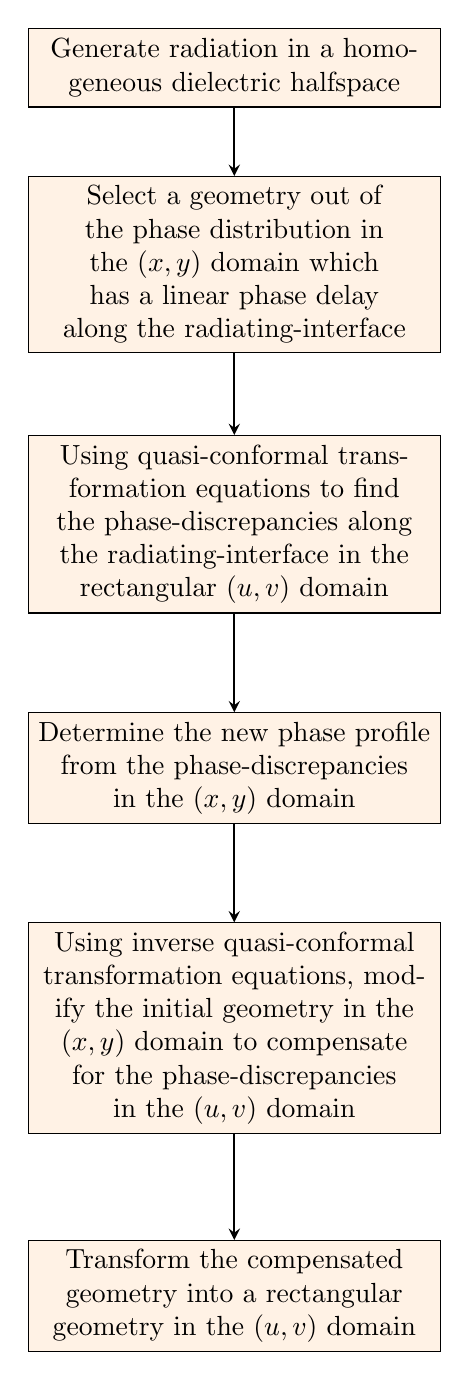
\begin{tikzpicture}[node distance=2cm]

\node (pro1) [rectangle, minimum width=3cm, minimum height=1cm, text centered, text width=5cm, draw=black, fill=orange!10] {Generate radiation in a homogeneous dielectric halfspace};
\node (pro2) [rectangle, minimum width=3cm, minimum height=1cm, text centered, text width=5cm, draw=black, fill=orange!10, below of=pro1, yshift=-.5cm] {Select a geometry out of the phase distribution in the $(x,y)$ domain which has a linear phase delay along the radiating-interface};
\node (pro3) [rectangle, minimum width=3cm, minimum height=1cm, text centered, text width=5cm, draw=black, fill=orange!10, below of=pro2, yshift=-1.3cm] {Using quasi-conformal transformation equations to find the phase-discrepancies along the radiating-interface in the rectangular $(u,v)$ domain};
\node (pro4) [rectangle, minimum width=3cm, minimum height=1cm, text centered, text width=5cm, draw=black, fill=orange!10, below of=pro3, yshift=-1.1cm] {Determine the new phase profile from the phase-discrepancies in the $(x,y)$ domain};
\node (pro5) [rectangle, minimum width=3cm, minimum height=1cm, text centered, text width=5cm, draw=black, fill=orange!10, below of=pro4, yshift=-1.3cm] {Using inverse quasi-conformal transformation equations, modify the initial geometry in the $(x,y)$ domain to compensate for the phase-discrepancies in the $(u,v)$ domain};
\node (pro6) [rectangle, minimum width=3cm, minimum height=1cm, text centered, text width=5cm, draw=black, fill=orange!10, below of=pro5, yshift=-1.4cm] {Transform the compensated geometry into a rectangular geometry in the $(u,v)$ domain};

\draw [thick,->,>=stealth] (pro1) -- (pro2);
\draw [thick,->,>=stealth] (pro2) -- (pro3);
\draw [thick,->,>=stealth] (pro3) -- (pro4);
\draw [thick,->,>=stealth] (pro4) -- (pro5);
\draw [thick,->,>=stealth] (pro5) -- (pro6);

\end{tikzpicture}

\end{center}
\caption{Algorithm of geometric compensation technique.}
\label{fig:flowchart}
\end{figure}
% Chapter 3
\chapter{Broad Band Fixed-beam Leaky Wave Antenna} % Main chapter title
\label{Chapter3} 
\renewcommand{\sectionmark}[1]{\markright{\thesection.\ #1}}
\chead{\rightmark}

The leaky-wave antenna presented in this thesis consists of two components: a slot-line array to generate the leaky-wave radiation and a rectangular graded dielectric superstrate placed on top of it. The superstate receives the generated leaky-wave radiation from the underlying slot array and couples it to free-space. The inhomogeneous distribution of permittivity inside the superstrate guides the wave to produce refraction at the upper interface at a specific angle. The geometric compensation technique presented in Sec. \ref{sec:geocomp} is employed in this chapter to design the rectangular slab. The chapter begins by describing the context of the fixed-beam radiation for the slot-array and proceeds to describe the design procedure. It is demonstrated that the geometric compensation technique decidedly improves the radiation characteristics of the antenna. A few variations of the proposed design are also presented in the final section of this chapter. 
%%%%%%%%%%%%%%%%%%%%%%%%%%%%%%%%%%%%%%%%%%%%%%%%%%%%%%%%%%%%%%%%%%%%%
\section{Design principle}
The design of the proposed leaky-wave antenna is influenced by the analysis of an infinitely long and optically narrow slot-line located at the interface between two different dielectric media \cite{Neto2003}\cite{Maci2004}. The radiation mechanism from such slot-lines is demonstrated in section \ref{SLLWA}. Figure \ref{fig:coupling}a is a similar illustration, showing a slot aperture extending in the positive $x$ direction and etched on a metallic ground plane in the $xy$ plane. A dielectric slab with a dielectric permittivity $\epsilon_r$ is located on top of the slot-line while the region underneath is free-space. If the slot aperture is transversely excited with a current element, a leaky-wave mode will propagate longitudinally in the direction of $x$ axis and continuously generate leaky-wave radiation into the dielectric slab. However, the generated leaky-wave radiation remains confined inside the superstrate due to total internal reflection at the air-dielectric interface, as illustrated by the ray-diagram in Fig. \ref{fig:coupling}a. 
%
\begin{figure} [t!]
\centering
\noindent
\hspace*{\fill}%
  \mbox{\subfloat[]
        {\begin{overpic}[scale=0.35]{Figures/Chapter3/fig_coupling/metaprism_1}
			\put(22,43){\footnotesize Uniform dielectric}
		\end{overpic}}}
	\hfill%
	\mbox{\subfloat[]
        {\begin{overpic}[scale=0.35]{Figures/Chapter3/fig_coupling/metaprism_2}
			\put(35,35){\footnotesize Uniform}
			\put(35,28){\footnotesize dielectric}
			\put(72,83){\footnotesize $\theta_{\mathrm{rad}}$}
		\end{overpic}}}
		\hspace*{\fill}%
		
	\mbox{\subfloat[]
        {\begin{overpic}[scale=0.35]{Figures/Chapter3/fig_coupling/metaprism_3}
			\put(42,62){\footnotesize $\theta_{\mathrm{rad}}$}
			\put(38,27){\footnotesize Graded index}
			\put(38,20){\footnotesize dielectric}	
			\put(-40,40){\vector(2,0){25}}
			\put(-40,40){\vector(0,2){25}}
			\put(-40,40){\vector(2,0){25}}
			\put(-40,40){\vector(3,2){20}}
			\put(-13,40){\footnotesize $x$}
			\put(-42,69){\footnotesize $y$}
			\put(-17,53){\footnotesize $z$}
			\put(130,40){\vector(2,0){25}}
			\put(130,40){\vector(0,2){25}}
			\put(130,40){\vector(2,0){25}}
			\put(130,40){\vector(3,2){20}}
			\put(157,40){\footnotesize $H_x$}
			\put(132,69){\footnotesize $H_y$}
			\put(151,53){\footnotesize $E_z$}
	\end{overpic}}}
  
  \caption[A diagram showing how a slot emitted leaky-wave radiation from a corner-fed slot-line leaky-wave antenna array remains trapped inside the uniform dielectric superstrate. A convex dielectric domain couples the generated radiation into free-space. The same phenomenon can be implemented with a rectangular graded-dielectric superstrate. ]{The slot emitted leaky-wave radiation from a corner-fed slot-line leaky-wave antenna array remains trapped inside the uniform dielectric superstrate (a). The phase-mismatch at the interface is reduced at a uniform dielectric convex layer which couples the generated radiation (b). The same phenomenon can be implemented with a rectangular graded-dielectric layer (c).  }
\label{fig:coupling}
\end{figure}
%
The incident angle (measured from broadside) of the leaky-wave at the upper interface of the uniform dielectric slab needs to be reduced in order to be coupled into free-space. This could be achieved by replacing the rectangular slab with a convex dielectric superstrate to couple the radiation into free-space through its curved upper interface, as shown in Fig. \ref{fig:coupling}b. The leaky-wave antenna reported in \cite{Neto2005} functioned with similar configuration. Here we seek to reduce the profile of the antenna and enable radiation in directions other than broadside.

Using transformation electromagnetics, the convex dielectric superstrate shown in Fig. \ref{fig:coupling}b is reshaped into an inhomogeneous rectangular one as shown Fig. \ref{fig:coupling}c. In contrast to the curved upper interface of the uniform dielectric medium in Fig. \ref{fig:coupling}b, the air-interface of the rectangular superstrate in Fig. \ref{fig:coupling}c is parallel to the slot-line. The inhomogeneous superstrate mimics the uniform dielectric hemisphere in Fig. \ref{fig:coupling}a and bends the slot-generated radiation to reduce its inident angle at the interface. The phase-profile of the wave along the upper interface of the superstrate determines the radiation angle of the leaky-wave antenna. The design process of the antenna involves obtaining the dimensions and permittivity distribution of the superstrate through transformation electromagnetics. 

%%%%%%%%%%%%%%%%%%%%%%%%%%%%%%%%%%%%%%%%%%%%%%%%%%%%%

\section{Design considerations} 
The leaky-wave antenna presented in this thesis consists of a slot-line array with a rectangular superstrate placed on top of it, as demonstrated in Fig. \ref{fig:coupling}c. The graded index dielectric superstate receives the generated leaky wave radiation from underlying the slot array and couple into free-space. The design of the antenna was conducted with an infinite slot array. The superstrate was consequently considered infinitely stretched in the direction transverse to the slot length, which aided saving computational resources by reducing the overall simulation domain.

The essential parameters considered for designing the leaky-wave antenna are:

\begin{itemize}
    \item The radiation angle: The fixed-beam leaky-wave antenna proposed by Neto \textit{et al.} was limited to broadside radiation \cite{Neto2005}\cite{Bruni2007}. The primary design criterion for the leaky-wave antenna is to produce a main beam at an oblique direction. The design procedure and simulation results presented in this chapter aims for a fixed radiation angle $\theta_{\mathrm{rad}} = 30^\circ$ from broadside. %This radiation angle was chosen to distinct the primary beam from the secondary lobes over the desired bandwidth. That being said, this angle can be chosen arbitrarily by the designer.
    
    \item Constituent material: The superstrate of the leaky-wave antenna consists of non-magnetic graded dielectric index material. The permittivity ($\epsilon$) of the slab is spatially distributed with unity permeability ($\mu$) value. The permittivity variation of the slab is two-dimensional with no variation in the direction transverse (the $z$ direction) to the slot-line. The superstrate was designed such that the value of relative permittivity ranges from 1 to 9. A maximum relative permittivity value of 9 was specifically chosen to limit the $\epsilon_r$ values to those of commonly available dielectrics. A maximum value of relative permittivity of 9 limits the refractive index value to 3. The minimum relative permittivity value was chosen to be unity because a relative permittivity below one would require artificial dielectrics which are either narrowband or require active elements. For instance, the antenna proposed by Sievenpiper consists of a dielectric substrate with relative permittivity below unity \cite{Sievenpiper2011}. However, the design utilizes active non-foster circuits to achieve fixed-beam radiation from the antenna. The design process of the antenna presented in this thesis was limited to passive devices only.
    
    \item Length of the antenna: In order to keep the antenna structure from being bulky, the length of the superstrate as well as the slot array was initially specified to be $L = 6 \lambda_0$, where $\lambda_0$ is the free-space wavelength. An antenna of such dimension is electromagnetically large for general applications. However, leaky-wave antennas are typically electromagnetically much long, typically around 10-12 wavelengths. It will be shown later that the desired antenna performance can be achieved from a length $L = 4.2 \lambda_0$, which is smaller than previous designs proposed by Neto \textit{et al.} and Sievenpiper.
    
    \item Frequency bandwidth: The objective was to achieve a percentage bandwidth over 100\%. While operating over a broad band, the antenna as well as the slot array becomes electrically smaller with the decrease of frequency. At lower frequencies, the leaky wave mode in the slot fails to radiate sufficient energy due to reduced length for propagation. This introduces reflections inside the slot that creates longitudinal reflections and interference inside the slot. As a result, the far-field radiation at lower frequencies contains higher sidelobe and wider beam at lower frequencies, as will be shown in later in section \ref{simres}. One way to get around this problem is to terminate the slot with a matched load so that the reflected waves do not interfere with the leaky-wave mode. In contrast to operation at lower frequencies, at higher frequencies, the antenna demonstrates improved performance in terms of sidelobe level and directivity because the antenna becomes electrically longer. We consider $2f_0$ for the upper frequency limit of the antenna, which leads to a length of $12 \lambda$ at the maximum frequency. The final design was simulated to have a fractional bandwidth of 5:1 where the sidelobe level remained below $30\%$ and the directivity was above 11.
\end{itemize}

\begin{figure}
\centering
 	\begin{overpic}[scale=0.7]{Figures/Chapter3/fig_structure/structure}
 	
 	        \put(-14,72){\footnotesize $2.9 \lambda_0$}
			\put(78,76){\footnotesize $4.2 \lambda_0$}
			\put(84,-5){\footnotesize $0.1 \lambda_0$}
			\put(57,-5){\footnotesize $0.02 \lambda_0$}
			\put(0,15){\footnotesize $v$}
			\put(7,28){\footnotesize $u$}
			\put(18,33){\footnotesize $z$}

  \end{overpic}

  \caption[The structure and physical dimensions of the simulated antenna.]{The structure and physical dimensions of the simulated antenna. All lengths are represented in terms of free-space wavelength $\lambda_0$ where frequency is $c$. The yellow substrate represents an inhomogeneous dielectric slab.}
\label{fig:structure}
\end{figure}

Hence the primary design criterion for the leaky-wave antenna was to produce a main beam at a fixed angle $\theta_{\mathrm{rad}} = 30^\circ$ over a wide-frequency range from $0.5f_0$ to $2f_0$. The designed antenna structure as well as the dimensions obtained through transformation electromagnetics is presented in Fig. \ref{fig:structure}. The slot width of the infinite slot array was specified to be $0.02 \lambda_0$ with an array spacing of $0.1 \lambda_0$. As will be shown, the antenna length and height was $4.2 \lambda_0$ and $2.9 \lambda_0$, respectively. 


%\section{Validation of Simulations}

%%%%%%%%%%%%%%%%%%%%%%%%%%%%%%%%%%%%%%%%%%%%%%%%%%%%%%%%%%%%%%%%%%%%%

%\label{App:NFTFF} describes validation process of the near field to far field process. 

\section{Design of the superstrate} \label{sec:design}
The rectangular superstrate of the leaky-wave antenna is designed using transformation optics along with the geometric compensation technique demonstrated in section \ref{sec:geocomp}. According to the technique, the rectangular shape of the superstrate is considered in the target domain. The graded permittivity distribution inside the superstrate is achieved through a two-step numerical conformal transformation process. 

\begin{figure} [t!]
\centering
  \noindent
\hspace*{1.5cm}
\mbox{\subfloat[]{
	\begin{overpic}[scale=0.4]{Figures/Chapter2/fig_simulation_domain/domain_corner}
			\put(42,18){\footnotesize L=6$\lambda$}
			\put(50,46){\footnotesize air}
			\put(50,73){\footnotesize dielectric}
			\put(-8,28){\footnotesize PEC}
	%		\put(-10,42){\footnotesize \fbox{PML}}
			\put(-16,39){\footnotesize Excitation}
			\put(08,90){\vector(-2,0){15}}
			\put(08,90){\vector(0,2){15}}
			\put(08,90){\vector(-2,0){15}}
			\put(08,90){\vector(3,4){8}}
			\put(-10,90){\footnotesize $y$}
			\put(5,105){\footnotesize $z$}
			\put(15,102){\footnotesize $x$}
	
  \end{overpic}}}
  \hspace*{1.5cm}%
    \mbox{\subfloat[]{
  
  	\begin{overpic}[scale=0.4]{Figures/Chapter2/fig_simulation_domain/domain2D}
        \put(50,87){\footnotesize L}
        \put(35,43){\footnotesize dielectric}
         \put(42,18){\footnotesize air}
  \end{overpic}}}
 \hspace*{2cm}% 
 

  \caption[Simulation setup for the analysis of the proposed leaky-wave antenna.]{Simulation setup for the analysis of the proposed leaky-wave antenna. Half of a unit cell is simulated with the PEC boundary conditions that extending the structure infinitely in the $z$ direction. The dashed region represents PML absorbing layer while the solid region is the actual simulation domain.}
\label{fig:simdomain2}
\end{figure}

\begin{figure} [t!]
\centering
  \noindent
  %
  \hspace*{\fill}%
 \mbox{\subfloat[]{
    	\begin{overpic}[trim={4cm -.6cm .6cm 1.2cm},clip,scale=0.3]{Figures/Chapter2/fig_simulation_domain/Ez1}
    			\put(70,0){\vector(2,0){10}}
    			\put(70,0){\vector(0,2){10}}
    			\put(80,01){\footnotesize $x$}
    			\put(70,11.5){\footnotesize $y$}
    			\put(68.5,-1.5){\footnotesize $\otimes$}
    			\put(66.5,-5){\footnotesize $z$}
    				\put(-4,47){\footnotesize \rotatebox{90}{$y (\lambda_0)$}}
    				\put(30,0){\footnotesize {$x (\lambda_0)$}}
    			
    			\linethickness{.7mm}
    			\put(15,90){\line(2,0){9}}
    			\put(16.5,92){\footnotesize $\lambda_0$}
    	
  \end{overpic}}}
  %
  %
   \mbox{\subfloat[]{
   	\begin{overpic}[trim={0cm 0cm .1cm 1cm},clip,scale=0.42, keepaspectratio=true]{Figures/Chapter2/fig_simulation_domain/Ez2}
  \end{overpic}}}
  \hspace*{\fill}%
  
  \hspace*{\fill}%
     \mbox{\subfloat[]{
   	\begin{overpic}[scale=0.5]{Figures/Chapter2/fig_simulation_domain/Ez3.png}
  \end{overpic}}}
  \hspace*{\fill}%
  %
  \caption[Fields produced in a uniform dielectric half-space that are used to determine the source domain geometry.]{(color inline) The fields produced in the structure demonstrated in Fig. \ref{fig:simdomain2} (a). The unwrapped phase (degrees) of the fields are plotted and used to determine the source domain geometry for the transformation optics procees. The blue lines correspond to the upper interface that corresponds to the phase profile being linear (b). The linear phase profile along the upper interface (c).}
\label{fig:simdomain2b}
\end{figure}

In the first step, an initial hypothetical geometry in the source domain is obtained through the technique shown in \ref{detsourcedom}. Using Eq. \ref{eq:lingrad}, a linear phase gradient is obtained which is a function of the radiation angle $\theta_{\mathrm{rad}}$ from broadside in the target domain. The achieved phase gradient is used to crop a shape out of a uniform dielectric half-space having a relative permittivity $\epsilon_r = 2$ is placed on top of a thin slot array. The scenario is simulated in COMSOL multiphysics. Figure \ref{fig:simdomain2} presents the simulation setup. An infinite array of slot-line etched on a ground plane placed at the interface of air and a dielectric was simulated using PEC/PMC symmetry planes and PML layers to mimic an infinite array located at the interface of two infinitely stretched half spaces. The solid lines represent the actual region of consideration while the dotted lines show the PML absorbing layers. They grey surface portrays the ground plane that holds a slot-line extended in the positive $\pm x$ direction. The slot-line is excited at the corner with a current source transverse to the length. The ground plane and the slot extends into the PML layer in the positive $\pm x$ direction. The PML layer absorbs the propagating leaky-wave mode in the slot-line and prevents reflections from boundary \cite{chew1995}. Standing waves originated from the reflected fields would cause error in determination of the source domain geometry.  In the negative $x$ direction there is an air gap between the PML boundary and round plane. The PML layer on the left of air gap infinitely extends the free-space region in in the negative $x$ direction, allowing simulation of a corner-fed leaky-wave antenna. The ground plane as well as the slot  perfect electric conductor (PEC) boundaries repeat the domain in the $\pm z$ direction, extending the structure into an infinite array \cite{sadiku2001}.

\begin{figure} [t!]
\centering
  \noindent
    \hspace*{\fill}%
  \mbox{\subfloat[]{
  \begin{overpic}[trim={0cm 0.0cm 0cm 0cm},clip,scale=0.35, keepaspectratio=true]{Figures/Chapter3/fig_transformation/phasecompensation_a}
				\put(3,-4){\footnotesize $z$}
				\put(10,45){\footnotesize $y$}
				\put(107,18){\footnotesize $x$}
				\put(53,77){\footnotesize Cut-line}
	\end{overpic}}}
\hspace*{\fill}%

\hspace*{\fill}%
\mbox{\subfloat[]{
  \begin{overpic}[trim={0cm 0.0cm 0cm 0cm},clip,scale=0.25, keepaspectratio=true]{Figures/Chapter3/fig_transformation/initial_source.png}
				\put(-4,53){\footnotesize $A$}
				\put(96,22){\footnotesize $B$}
				\put(-4,-5){\footnotesize $C$}
				\put(96,-6){\footnotesize $D$}
				\put(-10,-10){\vector(2,0){20}}
				\put(-10,-10){\vector(0,2){20}}
				\put(12,-12){\footnotesize $x$}
				\put(-12,15){\footnotesize $y$}
	\end{overpic}}}
\hspace*{\fill}%
  \mbox{\subfloat[]{
  \begin{overpic}[trim={0cm 0.2cm 0cm 0cm},clip,scale=0.25, keepaspectratio=true]{Figures/Chapter3/fig_transformation/initial_target.png}
				\put(-3,37){\footnotesize $a$}
				\put(97,37){\footnotesize $b$}
				\put(-3,0){\footnotesize $c$}
				\put(97,0){\footnotesize $d$}
				\put(-10,-10){\vector(2,0){20}}
				\put(-10,-10){\vector(0,2){20}}
				\put(12,-12){\footnotesize $u$}
				\put(-12,14){\footnotesize $v$}
				\put(7,47){\vector(2,0){88}}
				\put(95,47){\vector(-2,0){90}}
				\put(43.5,50){\footnotesize $L$}
				\put(105,0){\vector(0,2){42}}
				\put(105,42){\vector(0,-2){42}}
				\put(107,20){\footnotesize $H$}
	\end{overpic}}}
	  \hspace*{\fill}%
  \caption[Conformal transformation of the initial geometry into a rectangular domain.]{The initial geometry (a) that leads to a linear phase profile in the source domain. The conformal mapping from initial homogeneous source domain (b) to initial graded dielectric target domain (c).}
\label{fig:Geocomp}
\end{figure}

The transverse current source excitation of the slot-line generates a leaky-wave mode propagate in $x$ direction and radiates primarily into the upper dielectric half-space. Generated waves form a phase distribution in the dielectric half-space. The fields originated from the structure and the corresponding unwrapped phase are presented in Fig. \ref{fig:simdomain2b}a and \ref{fig:simdomain2b}b. The source domain geometry for the geometric compensation technique is selected using linear variation of phase with space. The electric field transverse to the length of the slot is considered to find the phase gradient from the dielectric half-space. The blue lines in Fig. \ref{fig:simdomain2b}b represent the upper interface that is selected using the linear phase profile in Fig. \ref{fig:simdomain2b}c. The upper interface of the source domain geometry designed with the intention of creating a linear phase profile, corresponding to a fixed radiation $\theta_{\mathrm{rad}}$ from broadside. Figure \ref{fig:Geocomp}a presents the geometry in the source domain which is determined for a radiation angle of $\theta_{\mathrm{rad}} = 30^\circ$. The overall design is carried out for a two-dimensional conformal transformation. Therefore, region under the upper interface (blue line) can be infinitely stretched in the $\pm z$ direction to find the domain in Fig. \ref{fig:Geocomp}a. The geometry with an infinite slot array at the bottom interface is presented in Fig. \ref{fig:Geocomp}a. The linear phase gradient along the upper interface of the geometry can be observed along a cut-line in the upper interface. 

For the two-dimensional conformal transformation, the geometries in figures \ref{fig:Geocomp}b and \ref{fig:Geocomp}c are considered. The shape $ABCD$ in \ref{fig:Geocomp}b is a portion of the uniform dielectric in the $xy$ plane along the cut-line indicating in Fig. \ref{fig:Geocomp}a. Using the description in section \ref{detsourcedom}, the geometry $ABCD$ is numerically mapped into a rectangle $abcd$ in $(u,v)$ domain presented in Fig. \ref{fig:Geocomp}c. The initial curved upper boundary is generated by setting the phase gradient along the curve equal to a constant. The constant is a function of the radiation angle from $ab$ in the target domain. The length of the target domain was specified to be $L = 6 \lambda_0$. Its height $H$, limited by the conformal module was $2.9 \lambda_0$. The permittivity distribution inside the rectangular medium is obtained from the transformation process. If the inhomogeneous rectangular superstrate is placed on top of the slot array used in the initial transformation process, generated leaky-wave radiation couples into free-space. The radiation angle depends on the phase-gradient along the upper interface $ab$. Due to the change of length of the upper boundary ($AB$ to $ab$), the phase gradient along $ab$ deviates from the expected linear profile. Figure \ref{fig:phaseini} presents the phase gradient along the radiating interface $ab$ in the target domain, which is clearly non-linear with repect to an ideal linear phase-profile. The non-linearity in phase profile along the interface leads unsatisfactory radiation patterns where the primary lobe deviates from the desired $30^\circ$ radiation angle and radiated power is significantly distributed in the side and back lobes. The linear radiation patterns from the structure are shown in Fig. \ref{fig:cornergeneral_uncomp} for a frequency range of $.5f_0$ to $2f_0$. The plot shows that although the the structure has been designed from a source domain for $30^\circ$ radiation, the primary beam deviates from the angle over the frequency range. 

\begin{figure} [t]
\pgfplotsset{compat=1.5,
scale=.9,
tick label style={font=\small},
label style={font=\small},
legend style={font=\small},
% tick style={thick}
}
  \begin{center}
 \begin{tikzpicture}
\pgfplotstableread[col sep=comma]{Figures/Chapter3/fig_smallercorner_polar/rectplot_freq4_uncomp.csv}{\loadeddatatwo}
\pgfplotstableread[col sep=comma]{Figures/Chapter3/fig_smallercorner_polar/rectplot_freq6_uncomp.csv}{\loadeddatathree}
\pgfplotstableread[col sep=comma]{Figures/Chapter3/fig_smallercorner_polar/rectplot_freq8_uncomp.csv}{\loadeddatafour}
\pgfplotstableread[col sep=comma]{Figures/Chapter3/fig_smallercorner_polar/rectplot_freq10_uncomp.csv}{\loadeddatafive}
\pgfplotstableread[col sep=comma]{Figures/Chapter3/fig_smallercorner_polar/rectplot_freq12_uncomp.csv}{\loadeddatasix}
\pgfplotstableread[col sep=comma]{Figures/Chapter3/fig_smallercorner_polar//rectplot_freq14_uncomp.csv}{\loadeddataseven}
\begin{polaraxis}[
  grid=both,
  legend pos=south east,
  major grid style={dotted},  
  minor grid style={dotted},  
  minor x tick num=1,
  minor y tick num=1,
 % title style={at={(0.5,0)},anchor=north,yshift=-25},
  %title = (a) Frequency {=} 1st Hz,
  xtick={0,30,...,330},
  extra x ticks={60},
  extra tick style={grid=major, grid style={solid, black, ultra thick}},
  %ytick={0,10,...,60},
  yticklabels={},
  ymin=0,
  ymax=70
]
%\addlegendentry{Uncompensated};
\addplot[
  data cs=polar,
  red,
  samples=500
] table[x index=0,y index=1] {\loadeddatatwo};
\addplot[
  data cs=polar,
  blue,
  samples=500
] table[x index=0,y index=1] {\loadeddatathree};
\addplot[
  data cs=polar,
  green,
  samples=500
] table[x index=0,y index=1] {\loadeddatafour};
\addplot[
  data cs=polar,
  yellow,
  samples=500
] table[x index=0,y index=1] {\loadeddatafive};
\addplot[
  data cs=polar,
  magenta,
  samples=500
] table[x index=0,y index=1] {\loadeddatasix};
\addplot[
  data cs=polar,
  black,
  samples=500
] table[x index=0,y index=1] {\loadeddataseven};
\addlegendentry{$f$ = $0.4 f_0$};
\addlegendentry{$f$ = $0.6 f_0$};
\addlegendentry{$f$ = $0.8 f_0$};
\addlegendentry{$f$ = $1.0 f_0$};
\addlegendentry{$f$ = $1.2 f_0$};
\addlegendentry{$f$ = $1.4 f_0$};
\end{polaraxis}
\end{tikzpicture}
 \end{center}
  \caption[Radiation patterns of the uncompensated leaky-wave antenna at different frequencies.]{(color inline) Radiation patterns (linear) of the uncompensated leaky-wave antenna at different frequencies. The six radiation patterns are for $0.5f_0$-$2f_0$, where $f_0=c$. Higher gain patters represents higher frequencies.}
\label{fig:cornergeneral_uncomp}
\end{figure}
%
\begin{figure} [t]
\pgfplotsset{compat=1.5,
width=7.5cm,
height=4.64cm,
tick label style={font=\small},
label style={font=\small},
legend style={font=\small},
% tick style={thick}
}
  \begin{center}
 \begin{tikzpicture}

\begin{axis}[transpose legend,
legend columns=1,
legend style={at={(0.82,1.2)},anchor=north},
cycle multi list={%
{red,mark={}},
{blue,solid,mark={}},
},
ymin=-22,
ymax=3,
xmin=0,
xmax=7,
xlabel={Arc length ($\lambda_0$)},
ylabel={Unwrapped phase (degrees)},
xtick={0,1,2,3,4,5,6,7},
%ytick={-1.4612e+03,-730.6029,0,730.6029,1.4612e+03},
xticklabels={$0$,$1$,$2$,$3$,$4$,$5$,$6$,$7$},
%title=Decay of Electric Field along the Single Slot and Slot Array under different dielectrics,
%xticklabel=\empty,
% yticklabel=\empty,
%xlabel={$Wave vector (K_{x}a_{x}/2\pi)$},
%ylabel={$Wave vector (K_{y}a_{y}/2\pi)$},
% extra x ticks={-78.54,78.54},
% extra y ticks={-78.54,78.54},
% extra x tick labels={$-0.0625$,$0.0625$},
% extra y tick labels={$-0.0625$,$0.0625$},
% smooth,
grid=major,
%legend entries={$\epsilon_r = 2$ (single slot),$\epsilon_r = 4$ (single slot),$\epsilon_r = 2$ (slot array),$\epsilon_r = 4$ (slot array)}
legend entries={Initial design, Ideal linear phase}
];
\addplot [thick, color=red, solid] table [col sep=comma] {Figures/Chapter3/fig_phase/uv_uncomp.csv};
%\addplot [thick, color=blue, solid] table [col sep=comma] {Figures/Chapter3/fig_phase/uv_comp.csv};
\addplot [thick, color=black, dashed] table [col sep=comma] {Figures/Chapter3/fig_phase/uv_ideal.csv};

\end{axis}
\end{tikzpicture}
 \end{center}
  \caption[Unwrapped phase profiles along the upper boundary of the uncompensated geometry in the target domain.]{Unwrapped phase profiles along the upper boundary of the initially transformed geometry. The dashed blue line presents the ideal linear phase gradient required.}
\label{fig:phaseini}
\end{figure}

In order to achieve a solid fixed-beam performance, the phase gradient along the upper interface of the superstrate needs to be precisely linear. In order to fix the discrepancies in the phase gradient, conformal transformation is required to be carried out. Using Eq. \ref{eq:comp}, a modified source domain is selected that leads to a different target domain medium. As described in the previous chapter, the modified geometry is selected from the unwrapped phase of the fields radiated into a uniform dielectric half-space. The red line in Fig. \ref{fig:phase}a presents upper interface of the compensated geometry, while the blue line is the initially selected interface (Fig. \ref{fig:simdomain2b}). 

The modified geometry with the slot array is presented in Fig. \ref{fig:LWAcompensation}a. A slice of the modified source domain along a cut-line is presented by geometry $A'B'C'D'$ in Fig. \ref{fig:LWAcompensation}b. The shape is mapped to the rectangular geometry $a'b'c'd'$ in Fig. \ref{fig:LWAcompensation}c through a two-dimensional conformal transformation. The geometry $a'b'c'd'$ is eventually used as the superstrate of the leaky-wave antenna superstrate. The domain has the same length $L$ as compared to the uncompensated one, however, has a height $H' = 2.9 \lambda_0$. 




%and presented in Fig. \ref{fig:LWAcompensation}a. The phase gradient along a cut line along the upper interface is not linear. However, the corresponding target domain has a linear phase profile along its upper interface.
\begin{figure} [t]
\centering
  \noindent
    \hspace*{\fill}%
\pgfplotsset{compat=1.5,
width=7cm,
height=6cm,
tick label style={font=\small},
label style={font=\small},
legend style={font=\small},
% tick style={thick}
}
\hspace*{\fill}%
  \mbox{\subfloat[]{
  \begin{overpic}[trim={4cm -.3cm 2.5cm 0cm},clip,scale=0.65, keepaspectratio=true]{Figures/Chapter3/fig_phase/Ez21_tricked}
  	\put(-4,52){\footnotesize \rotatebox{90}{$y (\lambda_0)$}}
  	\put(30,3){\footnotesize {$x (\lambda_0)$}}
		\end{overpic}}}
\hspace*{\fill}%    
  \mbox{\subfloat[]{
 \begin{tikzpicture}

\begin{axis}[transpose legend,
legend columns=1,
legend style={at={(0.80,1.1)},anchor=north},
cycle multi list={%
{red,mark={}},
{blue,solid,mark={}},
},
ymin=-22,
ymax=3,
xmin=0,
xmax=7,
xlabel={Arc length ($\lambda_0$)},
ylabel={Unwrapped phase (degrees)},
xtick={0,1,2,3,4,5,6,7},
%ytick={-1.4612e+03,-730.6029,0,730.6029,1.4612e+03},
xticklabels={$0$,$1$,$2$,$3$,$4$,$5$,$6$,$7$},
%title=Decay of Electric Field along the Single Slot and Slot Array under different dielectrics,
%xticklabel=\empty,
% yticklabel=\empty,
%xlabel={$Wave vector (K_{x}a_{x}/2\pi)$},
%ylabel={$Wave vector (K_{y}a_{y}/2\pi)$},
% extra x ticks={-78.54,78.54},
% extra y ticks={-78.54,78.54},
% extra x tick labels={$-0.0625$,$0.0625$},
% extra y tick labels={$-0.0625$,$0.0625$},
% smooth,
grid=major,
%legend entries={$\epsilon_r = 2$ (single slot),$\epsilon_r = 4$ (single slot),$\epsilon_r = 2$ (slot array),$\epsilon_r = 4$ (slot array)}
legend entries={Initial design, Compensated geometry, Ideal linear phase}
];
\addplot [thick, color=red, solid, mark = square,mark indices={1,300,600,900,1200,1401}] table [col sep=comma] {Figures/Chapter3/fig_phase/uv_uncomp.csv};
\addplot [thick, color=blue, solid, mark = o,mark indices={1,300,600,900,1200,1401}] table [col sep=comma] {Figures/Chapter3/fig_phase/uv_comp.csv};
\addplot [thick, color=black, dashed] table [col sep=comma] {Figures/Chapter3/fig_phase/uv_ideal.csv};

\end{axis}
\end{tikzpicture} }}
     \hspace*{\fill}%
  \caption[Compensating the source domain geometry using the corrected phase-profile.] {(color inline) Determining the compensated geometry from the surface plot of phase (degrees) corresponding to the fields in an uniform dielectric half-space(a). Unwrapped phase profiles along the upper boundaries of the initial and compensated geometry (b).}
\label{fig:phase}
\end{figure}

The blue curve in Fig. \ref{fig:phase}a demonstrates how the phase profile along the upper boundary $ab$ is more linear as compared to the initial design. The plot illustrates how the linearity in phase-profile along the radiating interface improves after applying the geometric compensation technique. As will be shown in section \ref{simres}, the geometrically compensated target domain $a'b'c'd'$ demonstrates improved antenna perforamnce as cormpared to the initially designed medium $abcd$.
\begin{figure} [t!]
\centering
  \noindent
    \hspace*{\fill}%
 \mbox{\subfloat[]{
  \begin{overpic}[trim={0cm 0.0cm 0cm 0cm},clip,scale=0.30, keepaspectratio=true]{Figures/Chapter3/fig_transformation/phasecompensation_b}
			
				\put(3,-4){\footnotesize $w$}
				\put(10,45){\footnotesize $v$}
				\put(105,13){\footnotesize $u$}
				\put(53,77){\footnotesize Cut-line}
	\end{overpic}}}
\hspace*{\fill}%

\hspace*{\fill}%
	\noindent
	\mbox{\subfloat[]{
  \begin{overpic}[trim={0cm 0.0cm 0cm 0cm},clip,scale=0.25, keepaspectratio=true]{Figures/Chapter3/fig_transformation/compensated_source.png}
				\put(-4,50){\footnotesize $A'$}
				\put(94,20){\footnotesize $B'$}
				\put(-4,-2){\footnotesize $C'$}
				\put(94,-2){\footnotesize $D'$}
				\put(-10,-10){\vector(2,0){20}}
				\put(-10,-10){\vector(0,2){20}}
				\put(12,-12){\footnotesize $x$}
				\put(-12,14){\footnotesize $y$}
	\end{overpic}}}
\hspace*{\fill}%
  \mbox{\subfloat[]{
  \begin{overpic}[trim={0cm 1.8cm 0cm 0cm},clip,scale=0.25, keepaspectratio=true]{Figures/Chapter3/fig_transformation/compensated_target.png}
			    \put(-2,30){\footnotesize $a'$}
				\put(93,30){\footnotesize $b'$}
				\put(-2,0){\footnotesize $c'$}
				\put(93,0){\footnotesize $d'$}
				\put(-10,-10){\vector(2,0){20}}
				\put(-10,-10){\vector(0,2){20}}
				\put(12,-12){\footnotesize $u$}
				\put(-12,14){\footnotesize $v$}
				\put(9,42){\vector(2,0){81}}
				\put(87,42){\vector(-2,0){81}}
				\put(46,45){\footnotesize $L$}
				\put(105,2){\vector(0,2){33}}
				\put(105,35){\vector(0,-2){33}}
				\put(107,17.5){\footnotesize $H'$}
	\end{overpic}}}
	  \hspace*{\fill}%
  \caption[The compensated source domain geometry and its transformation to rectangular target domain.] {The compensated geometry (a) that leads to a linear phase profile in the target domain. The conformal mapping from geometrically-compensated homogeneous source domain (b) to geometrically compensated graded dielectric target domain (c).}
\label{fig:LWAcompensation}
\end{figure}


It is observed that the relative permittivity inside the superstrate varies from 0.0790 to 8.8748, as shown in the countour plot of Fig. \ref{fig:permittivity}. Naturally occurring dielectric materials generally have a refractive index greater than unity. Media having a relative permittivity bellow unity needs to be implemented using resonant materials which are narrowband. In order to avoid resonant materials, the region with relative permittivity below 1 were approximated to be 1. The region with unity relative permittivity was distributed along the last end of the superstrate, as illustrated in Fig. \ref{fig:permittivity}. This effectively trimmed the physical length of the superstrate from $L=6 \lambda_0$ to $L=4.2 \lambda_0$, causing an drop in directivity and increase in sidelobe levels.% \textcolor{red}{do you have percentage change?}.
\begin{figure} [t!]
\centering
 	\begin{overpic}[scale=0.8]{Figures/Chapter3/fig_permittivity/corner_fed.png}

  \end{overpic}

  \caption[Permittivity distribution inside the geometrically compensated superstate in the target domain.]{Permittivity distribution inside the geometrically compensated superstate in the target domain.}
\label{fig:permittivity}
\end{figure}

The fields in the target domain $a'b'c'd'$ in Fig. \ref{fig:LWAcompensation}c are re-simulated in the next section with a slot array placed at the bottom interface $c'd'$. The array is specified by a slot spacing of $\lambda_0/10$, slot width of $\lambda_0/50$, and slot length of $6\lambda_0$, where $\lambda_0$ is the free-space wavelength. 


%%%%%%%%%%%%%%%%%%%%%%%%%%%%%%%%%%%%%%%%%%%%%%%%%%%%%%%%%%%%%%%%%%%%%%%%
\section{Antenna performance} \label{simres}
The leaky-wave antenna is designed as described in section \ref{sec:design} and simulated using COMSOL Multiphysics. The simulated antenna consisted of a corner-fed infinite slot array with a graded index dielectric superstrate on top, similar to the structure shown in Fig. \ref{fig:coupling}c. The rectangular superstrate is designed through transformation optics to linearize the phase along the air-dielectric interface. 

\subsection{Fixed-beam broad band performance}
\begin{figure} [t!]
\centering
 	\begin{overpic}[trim={0.5cm -0.5cm 0.5cm 1.4cm},clip,scale=0.35]{Figures/Chapter3/fig_permittivity/Ez.png}

\put(1,41){\footnotesize \rotatebox{90}{$v (\lambda_0)$}}
\put(37,0){\footnotesize {$u (\lambda_0)$}}
  \end{overpic}

  \caption[Simulated electric field of the designed fixed-beam leaky-wave antenna.]{(color inline) Simulated electric field transverse to the slot. The slot generated leaky-wave radiation bends towards the higher permittivity region and couples into free-space.}
\label{fig:field}
\end{figure}
\begin{figure} [h!]
\pgfplotsset{compat=1.5,
scale=.9,
tick label style={font=\small},
label style={font=\small},
legend style={font=\small},
% tick style={thick}
}
  \begin{center}
 \begin{tikzpicture}
\pgfplotstableread[col sep=comma]{Figures/Chapter3/fig_smallercorner_polar/rectplot_freq4_comp.csv}{\loadeddatatwo}
\pgfplotstableread[col sep=comma]{Figures/Chapter3/fig_smallercorner_polar/rectplot_freq6_comp.csv}{\loadeddatathree}
\pgfplotstableread[col sep=comma]{Figures/Chapter3/fig_smallercorner_polar/rectplot_freq8_comp.csv}{\loadeddatafour}
\pgfplotstableread[col sep=comma]{Figures/Chapter3/fig_smallercorner_polar/rectplot_freq10_comp.csv}{\loadeddatafive}
\pgfplotstableread[col sep=comma]{Figures/Chapter3/fig_smallercorner_polar/rectplot_freq12_comp.csv}{\loadeddatasix}
\pgfplotstableread[col sep=comma]{Figures/Chapter3/fig_smallercorner_polar//rectplot_freq14_comp.csv}{\loadeddataseven}
\begin{polaraxis}[
  grid=both,
  legend pos=south east,
  major grid style={dotted},  
  minor grid style={dotted},  
  minor x tick num=1,
  minor y tick num=1,
 % title style={at={(0.5,0)},anchor=north,yshift=-25},
  %title = (a) Frequency {=} 1st Hz,
  xtick={0,30,...,330},
  extra x ticks={60},
  extra tick style={grid=major, grid style={solid, black, ultra thick}},
  %ytick={0,10,...,60},
  yticklabels={},
  ymin=0,
  ymax=96
]
%\addlegendentry{Uncompensated};
\addplot[
  data cs=polar,
  red,
  samples=500
] table[x index=0,y index=1] {\loadeddatatwo};
\addplot[
  data cs=polar,
  blue,
  samples=500
] table[x index=0,y index=1] {\loadeddatathree};
\addplot[
  data cs=polar,
  green,
  samples=500
] table[x index=0,y index=1] {\loadeddatafour};
\addplot[
  data cs=polar,
  yellow,
  samples=500
] table[x index=0,y index=1] {\loadeddatafive};
\addplot[
  data cs=polar,
  magenta,
  samples=500
] table[x index=0,y index=1] {\loadeddatasix};
\addplot[
  data cs=polar,
  black,
  samples=500
] table[x index=0,y index=1] {\loadeddataseven};
\addlegendentry{$f$ = $0.4 f_0$};
\addlegendentry{$f$ = $0.6 f_0$};
\addlegendentry{$f$ = $0.8 f_0$};
\addlegendentry{$f$ = $1.0 f_0$};
\addlegendentry{$f$ = $1.2 f_0$};
\addlegendentry{$f$ = $1.4 f_0$};
\end{polaraxis}
\end{tikzpicture}
 \end{center}
  \caption[Radiation patterns of the compensated leaky-wave antenna at different frequencies.]{(color inline) Radiation patterns (linear) of the compensated leaky-wave antenna at different frequencies. The six radiation patterns are for $0.5f_0$-$2f_0$, where $f_0=c$. Higher gain patters represents higher frequencies.}
\label{fig:cornergeneral}
\end{figure}
%
Fig. \ref{fig:field} depicts how the fields bend inside the graded dielectric index substrate and subsequently couple into free-space. Interference of fields is visible inside the superstrate which is originated from the reflection at the air-dielectric interface. The oblique radiation of the leaky-wave is visible from the coupled waves. Figure \ref{fig:cornergeneral} illustrates linear radiation patterns of the antenna over broad bandwidth. The six curves represent the radiation patterns from $.5f_0$ to $2f_0$ ($f_0=c$). The plot shows that the structure generates a primary beam directed approximately at the same angle, at $30^\circ$ from broadside in this case. 

\subsection{Improvement of radiation pattern using geometric compensation technique}

\begin{figure} [t!]
\pgfplotsset{compat=1.5,
scale=.58,
tick label style={font=\small},
label style={font=\small},
legend style={font=\small},
% tick style={thick}
}
  \begin{center}

 \begin{tikzpicture}[scale=\scalingfactor]
\pgfplotstableread[col sep=comma]{Figures/Chapter3/fig_smallercorner_polar/rectplot_freq2_comp.csv}{\loadeddataone}
\pgfplotstableread[col sep=comma]{Figures/Chapter3/fig_smallercorner_polar/rectplot_freq2_uncomp.csv}{\loadeddatatwo}
\begin{polaraxis}[
  grid=both,
  legend pos=south west,
  major grid style={dotted},  
  minor grid style={dotted},  
  minor x tick num=1,
  minor y tick num=1,
  title style={at={(0.5,0)},anchor=north,yshift=-25},
  title = (a) Frequency {=} $0.5f_0$,
  xtick={0,30,...,330},
  extra x ticks={60},
  extra tick style={grid=major, grid style={solid, black, ultra thick}},
%  ytick={0,10,...,60},
  yticklabels={},
  ymin=0,
  ymax=1
]
%\addlegendentry{Uncompensated};
\addplot[
  data cs=polar,
  red,
  samples=500
] table[x index=0,y index=2] {\loadeddatatwo};
\addplot[
  data cs=polar,
  blue,
  samples=500
] table[x index=0,y index=2] {\loadeddataone};
%\addlegendentry{Compensated};
\end{polaraxis}
\end{tikzpicture}
  \hspace*{\fill}%
  \begin{tikzpicture}[scale=\scalingfactor]
\pgfplotstableread[col sep=comma]{Figures/Chapter3/fig_smallercenter_polar/radiation_pattern_comp_4.csv}{\loadeddataone}
\pgfplotstableread[col sep=comma]{Figures/Chapter3/fig_smallercenter_polar/radiation_pattern_uncomp_4.csv}{\loadeddatatwo}
\pgfplotstableread[col sep=comma]{Figures/Chapter3/fig_smallercenter_polar/reflector_radiation_pattern_comp_4.csv}{\loadeddatathree}
\begin{polaraxis}[
  grid=both,
  legend pos=south west,
  major grid style={dotted},  
  minor grid style={dotted},  
  minor x tick num=1,
  minor y tick num=1,
  title style={at={(0.5,0)},anchor=north,yshift=-25},
  title = (b) Frequency {=} $0.8f_0$,
  xtick={0,30,...,330},
  ytick={0,10,...,60},
  extra x ticks={60},
  extra tick style={grid=major, grid style={solid, black, ultra thick}},
  yticklabels={},
  ymin=0,
  ymax=1
]
%\addlegendentry{Uncompensated};
\addplot[
  data cs=polar,
  red,
  samples=500
] table[x index=0,y index=2] {\loadeddatatwo};
\addplot[
  data cs=polar,
  blue,
  samples=500
] table[x index=0,y index=2] {\loadeddataone};
\addplot[
  data cs=polar,
  dgreen,
  samples=500
] table[x index=0,y index=2] {\loadeddatathree};
%\addlegendentry{Compensated};
\end{polaraxis}
\end{tikzpicture}

  

  \begin{tikzpicture}[scale=\scalingfactor]
\pgfplotstableread[col sep=comma]{Figures/Chapter3/fig_smallercenter_polar/radiation_pattern_comp_8.csv}{\loadeddataone}
\pgfplotstableread[col sep=comma]{Figures/Chapter3/fig_smallercenter_polar/radiation_pattern_uncomp_8.csv}{\loadeddatatwo}
\pgfplotstableread[col sep=comma]{Figures/Chapter3/fig_smallercenter_polar/reflector_radiation_pattern_comp_8.csv}{\loadeddatathree}
\begin{polaraxis}[
  grid=both,
  legend pos=south west,
  major grid style={dotted},  
  minor grid style={dotted},  
  minor x tick num=1,
  minor y tick num=1,
  title style={at={(0.5,0)},anchor=north,yshift=-25},
  title = (c) Frequency {=} $1.2f_0$,
  xtick={0,30,...,330},
  ytick={0,10,...,60},
  extra x ticks={60},
  extra tick style={grid=major, grid style={solid, black, ultra thick}},
  yticklabels={},
  ymin=0,
  ymax=1
]
%\addlegendentry{Uncompensated};
\addplot[
  data cs=polar,
  red,
  samples=500
] table[x index=0,y index=2] {\loadeddatatwo};
\addplot[
  data cs=polar,
  blue,
  samples=500
] table[x index=0,y index=2] {\loadeddataone};
\addplot[
  data cs=polar,
  dgreen,
  samples=500
] table[x index=0,y index=2] {\loadeddatathree};
%\addlegendentry{Compensated};
\end{polaraxis}
\end{tikzpicture}
  \hspace*{\fill}%
  \begin{tikzpicture}[scale=\scalingfactor]
\pgfplotstableread[col sep=comma]{Figures/Chapter3/fig_smallercenter_polar/radiation_pattern_comp_10.csv}{\loadeddataone}
\pgfplotstableread[col sep=comma]{Figures/Chapter3/fig_smallercenter_polar/radiation_pattern_uncomp_10.csv}{\loadeddatatwo}
\pgfplotstableread[col sep=comma]{Figures/Chapter3/fig_smallercenter_polar/reflector_radiation_pattern_comp_10.csv}{\loadeddatathree}
\begin{polaraxis}[
  grid=both,
  legend pos=south west,
  major grid style={dotted},  
  minor grid style={dotted},  
  minor x tick num=1,
  minor y tick num=1,
  title style={at={(0.5,0)},anchor=north,yshift=-25},
  title = (d) Frequency {=} $1.4f_0$,
  xtick={0,30,...,330},
  ytick={0,10,...,60},
  extra x ticks={60},
  extra tick style={grid=major, grid style={solid, black, ultra thick}},
  yticklabels={},
  ymin=0,
  ymax=1
]
%\addlegendentry{Uncompensated};
\addplot[
  data cs=polar,
  red,
  samples=500
] table[x index=0,y index=2] {\loadeddatatwo};
\addplot[
  data cs=polar,
  blue,
  samples=500
] table[x index=0,y index=2] {\loadeddataone};
\addplot[
  data cs=polar,
  dgreen,
  samples=500
] table[x index=0,y index=2] {\loadeddatathree};
%\addlegendentry{Compensated};
\end{polaraxis}
\end{tikzpicture}

  

  \begin{tikzpicture}[scale=\scalingfactor]
\pgfplotstableread[col sep=comma]{Figures/Chapter3/fig_smallercorner_polar/rectplot_freq12_comp.csv}{\loadeddataone}
\pgfplotstableread[col sep=comma]{Figures/Chapter3/fig_smallercorner_polar/rectplot_freq12_uncomp.csv}{\loadeddatatwo}
\begin{polaraxis}[
  grid=both,
  legend pos=south west,
  major grid style={dotted},  
  minor grid style={dotted},  
  minor x tick num=1,
  minor y tick num=1,
  title style={at={(0.5,0)},anchor=north,yshift=-25},
  title = (e) Frequency {=} $1.6f_0$,
  xtick={0,30,...,330},
  extra x ticks={60},
  extra tick style={grid=major, grid style={solid, black, ultra thick}},
%  ytick={0,10,...,60},
  yticklabels={},
  ymin=0,
  ymax=1
]
%\addlegendentry{Uncompensated};
\addplot[
  data cs=polar,
  red,
  samples=500
] table[x index=0,y index=2] {\loadeddatatwo};
\addplot[
  data cs=polar,
  blue,
  samples=500
] table[x index=0,y index=2] {\loadeddataone};
%\addlegendentry{Compensated};
\end{polaraxis}
\end{tikzpicture}
  \hspace*{\fill}%
  \begin{tikzpicture}[scale=\scalingfactor]
\pgfplotstableread[col sep=comma]{Figures/Chapter3/fig_smallercenter_polar/radiation_pattern_comp_16.csv}{\loadeddataone}
\pgfplotstableread[col sep=comma]{Figures/Chapter3/fig_smallercenter_polar/radiation_pattern_uncomp_16.csv}{\loadeddatatwo}
\pgfplotstableread[col sep=comma]{Figures/Chapter3/fig_smallercenter_polar/reflector_radiation_pattern_comp_16.csv}{\loadeddatathree}
\begin{polaraxis}[
  grid=both,
  legend pos=south west,
  major grid style={dotted},  
  minor grid style={dotted},  
  minor x tick num=1,
  minor y tick num=1,
  title style={at={(0.5,0)},anchor=north,yshift=-25},
  title = (f) Frequency {=} $2f_0$,
  xtick={0,30,...,330},
  ytick={0,10,...,60},
  extra x ticks={60},
  extra tick style={grid=major, grid style={solid, black, ultra thick}},
  yticklabels={},
  ymin=0,
  ymax=1
]
%\addlegendentry{Uncompensated};
\addplot[
  data cs=polar,
  red,
  samples=500
] table[x index=0,y index=2] {\loadeddatatwo};
\addplot[
  data cs=polar,
  blue,
  samples=500
] table[x index=0,y index=2] {\loadeddataone};
\addplot[
  data cs=polar,
  dgreen,
  samples=500
] table[x index=0,y index=2] {\loadeddatathree};
%\addlegendentry{Compensated};
\end{polaraxis}
\end{tikzpicture}

 \end{center}
  \caption[Normalized radiation patterns for the initial and compensated (blue) corner-fed leaky-wave antenna at particular frequencies.]{(color inline) Normalized radiation patterns for the initial (red) and compensated (blue) leaky-wave antenna at different frequencies.}
\label{fig:cornerpolar}
\end{figure}
%
\begin{figure} [t!]
	\pgfplotsset{compat=1.5,
		width=20cm,
		height=5.2cm,
		scale=.8,
		tick label style={font=\small},
		label style={font=\small},
		legend style={font=\small},
		% tick style={thick}
	}
	\begin{center}
		\begin{tikzpicture}
   \begin{groupplot}[group style={
                      group name=myplot,
                      group size= 1 by 5, horizontal sep=2cm, vertical sep=1.0cm},height=3.5cm, width=7.5cm]
     
 
         \nextgroupplot[ymin=20,
ymax=55,
title style={at={(0.5,0)},anchor=north,yshift=-10,xshift=70},
title = (a),
%xlabel={Frequency},
ylabel={$\theta_{rad}$ (deg)},
xtick={2e8,3e8,4e8,5e8,6e8},
xticklabels={$0.65f_0$,$f_0$,$1.35f_0$,$1.65f_0$,$2f_0$},
        scaled x ticks = false,     
        x tick label style={rotate=45, anchor=east},
]

             %   \addplot[blue, thick, mark = square]table [col sep=comma]  {A_radiation_angle.csv};\label{plots:plot1}
             %   \addplot[dgreen, thick, mark = x]table [col sep=comma]  {A_radiation_angle_reflector.csv};\label{plots:plot2}
             %   \addplot[red, thick, mark=o] table [col sep=comma] {A_radiation_angle_uncomp.csv};\label{plots:plot3}
                
                \addplot[blue, thick, mark = square]table [col sep=comma]  {Figures/Chapter3/fig_smallercorner_characterize/A_corner_radiation_angle.csv};\label{plots:plot4}
                \addplot[red, thick, mark=o] table [col sep=comma] {Figures/Chapter3/fig_smallercorner_characterize/A_corner_radiation_angle_uncomp.csv};\label{plots:plot5}


                \addplot[mark=none, ultra thick, dashed, black, samples=2] coordinates {(1.5e8,33) (6e8,33)};

                       
        \nextgroupplot[ymin=5,
ymax=35,
%xlabel={Frequency},
title style={at={(0.5,0)},anchor=north,yshift=-10,xshift=70},
title = (b),
ylabel={3dB BW (deg)},
xtick={2e8,3e8,4e8,5e8,6e8},
xticklabels={$0.65f_0$,$f_0$,$1.35f_0$,$1.65f_0$,$2f_0$},
        scaled x ticks = false,          x tick label style={rotate=45, anchor=east},
]


              %  \addplot[blue, thick, mark = square] table [col sep=comma] {B_3db_beamwidth.csv};
             %   \addplot[dgreen, thick, mark = x] table [col sep=comma] {B_3db_beamwidth_reflector.csv};
              %  \addplot[red, thick, mark=o] table [col sep=comma]  {B_3db_beamwidth_uncomp.csv};
                
                \addplot[blue, thick, mark = square]table [col sep=comma]  {Figures/Chapter3/fig_smallercorner_characterize/B_corner_3db_beamwidth.csv};
                \addplot[red, thick, mark=o] table [col sep=comma] {Figures/Chapter3/fig_smallercorner_characterize/B_corner_3db_beamwidth_uncomp.csv};




        
        \nextgroupplot[ymin=5,
ymax=95,
%xlabel={Frequency},
title style={at={(0.5,0)},anchor=north,yshift=-10,xshift=70},
title = (c),
ylabel={SLL ($\%$)},
xtick={2e8,3e8,4e8,5e8,6e8},
xticklabels={$0.65f_0$,$f_0$,$1.35f_0$,$1.65f_0$,$2f_0$},
        scaled x ticks = false,          x tick label style={rotate=45, anchor=east},
]

              %  \addplot[blue, thick, mark = square]  table [col sep=comma]{C_sidelobe.csv};
              %  \addplot[dgreen, thick, mark = x]  table [col sep=comma]{C_sidelobe_reflector.csv};
             %   \addplot[red, thick, mark=o]  table [col sep=comma] {C_sidelobe_uncomp.csv};
                
                 \addplot[blue, thick, mark = square]table [col sep=comma]  {Figures/Chapter3/fig_smallercorner_characterize/C_corner_sidelobe.csv};
                \addplot[red, thick, mark=o] table [col sep=comma] {Figures/Chapter3/fig_smallercorner_characterize/C_corner_sidelobe_uncomp.csv};



 
        
        \nextgroupplot[ymin=25,
ymax=100,
%xlabel={Frequency},
title style={at={(0.5,0)},anchor=north,yshift=-10,xshift=70},
title = (d),
ylabel={BLL ($\%$)},
xtick={2e8,3e8,4e8,5e8,6e8},
xticklabels={$0.65f_0$,$f_0$,$1.35f_0$,$1.65f_0$,$2f_0$},
        scaled x ticks = false,          x tick label style={rotate=45, anchor=east},
]

             %   \addplot[blue, thick, mark = square] table [col sep=comma] {D_backlobe.csv};
             %   \addplot[dgreen, thick, mark = x] table [col sep=comma] {D_backlobe_reflector.csv};
            %    \addplot[red, thick, mark=o] table [col sep=comma]  {D_backlobe_uncomp.csv};
            
                \addplot[blue, thick, mark = square]table [col sep=comma]  {Figures/Chapter3/fig_smallercorner_characterize/D_corner_backlobe.csv};
                \addplot[red, thick, mark=o] table [col sep=comma] {Figures/Chapter3/fig_smallercorner_characterize/D_corner_backlobe_uncomp.csv};
                



 
 
    \nextgroupplot[ymin=0,
ymax=25,
xlabel={Frequency },
ylabel={Directivity (linear)},
title style={at={(0.5,0)},anchor=north,yshift=-10,xshift=70},
title = (e),
xtick={2e8,3e8,4e8,5e8,6e8},
xticklabels={$0.65f_0$,$f_0$,$1.35f_0$,$1.65f_0$,$2f_0$},
        scaled x ticks = false,          x tick label style={rotate=45, anchor=east},
]

              %  \addplot[blue, thick, mark = square] table [col sep=comma] {E_directivity.csv};
              %  \addplot[dgreen, thick, mark = x] table [col sep=comma] {E_directivity_reflector.csv};
             %   \addplot[red, thick, mark=o] table [col sep=comma]  {E_directivity_uncomp.csv};
                
                \addplot[blue, thick, mark = square]table [col sep=comma]  {Figures/Chapter3/fig_smallercorner_characterize/E_corner_directivity.csv};
                \addplot[red, thick, mark=o] table [col sep=comma] {Figures/Chapter3/fig_smallercorner_characterize/E_corner_directivity_uncomp.csv};
                
                
            
                
    \end{groupplot}


   
   % \path (myplot c1r1.outer north west)% plot in column 1 row 1
   %       -- node[anchor=south,rotate=90] {throughput}% label midway
      %    (myplot c1r2.outer south west)% plot in column 1 row 4
    ;
% legend
\path (myplot c1r1.north|-current bounding box.north)-- 
      coordinate(legendpos)
      (myplot c1r1.south|-current bounding box.north);
\matrix[
    matrix of nodes,
    anchor=south,
    draw,
    inner sep=0.2em,
    draw
  ]at([yshift=2ex]legendpos)
  { %\ref{plots:plot1}& Compensated: Centre-fed &[5pt]\\
  %  \ref{plots:plot2}& Compensated: Centre-fed with Back Reflector &[5pt]\\
    \ref{plots:plot4}& Compensated: Corner-fed  &[5pt]\\
   % \ref{plots:plot3}& Uncompensated: Centre-fed &[5pt]\\
    \ref{plots:plot5}& Uncompensated: Corner-fed &[5pt]\\};
\end{tikzpicture}
	\end{center}
  \caption[Characterization plots comparing the angle of radiation, sidelobe level, backlobe level, 3dB beamwidth and directivity of the corner-fed antenna over a broad bandwidth.]{(color inline) (a) Radiated beam angle, (b) 3dB beam width, (c) sidelobe level, (d) backlobe level and (e) directivity of the leaky-wave antenna for the geometrically compensated superstrate (blue) and initially designed superstrate (red). The dashed black line in (a) represents the average beam angle of $33^o$.}
\label{fig:cornerradpattern}
\end{figure}

%
To compare the performance of the antenna at different frequencies, normalized radiation patterns at different frequencies need to be compared. Normalized radiation patterns at different frequencies comparing the initial design and the compensated design is presented in Fig. \ref{fig:cornerpolar}. The blue and red curves presents the far-field radiation pattern for the geometrically compensated and initial design, respectively. The normalized radiation patterns illustrates how the performance of the antenna increases with the increase of frequency. At higher frequencies, the electrical antenna structure is long enough to allow the leaky-wave mode in the slot to decay. However, the antenna structure becomes electrically smaller at lower frequencies. The propagating leaky-wave mode is strong enough at the end of the structure is strong enough to cause significant standing wave components in the slot. Therefore the antenna performance degrades at lower frequencies. Regardless of higher sidelobe and backlobe levels at lower frequencies, the primary beam remains at the designed angle ($\theta_{\mathrm{rad}} = 30^\circ$ from broadside).

Fig. \ref{fig:cornerradpattern} presents the parameters of the simulated leaky-wave antenna with the geometrically compensated superstrate and the initial design. Simulated radiation angle, 3dB beamwidth, percentage sidelobe level, percentage backlobe level and directivity of the antenna at different frequencies for both initial and geometrically compensated design. As illustrated in Fig. \ref{fig:cornerradpattern}a, the radiation angle for the compensated superstrate remain consistent as compared to the initial design, fluctuating around the designed $30$ degrees over the desired bandwidth. According to in Fig. \ref{fig:cornerradpattern}b, 3dB beamwidth for the compensated design is relatively less than the initial design and follows a downward trend with the increase of frequency. The sidelobe level (Fig. \ref{fig:cornerradpattern}c) and backlobe level (Fig. \ref{fig:cornerradpattern}d) graphs show the percentage sidelobe and backlobe level for the compensated design is reasonably less than that for the initial design throughout the frequency range. At the lower cut-off frequency the simulated sidelobe level and backlobe level are $37.3\%$ and $79.8\%$, respectively for the compensated superstrate while results for the same antenna parameters initial design are $46.4\%$ and $91.6\%$, respectively. The percentage sidelobe level and  backlobe level marginally decrease to $30\%$ and $46\%$for the compensated superstrate, being lower than the initial design over the frequency range. As for the directivity of the leaky-wave antenna in Fig. \ref{fig:cornerradpattern}e, it shows an upward trend with the increase of frequency for both designs. The compensated design generates more directive beam over the range of frequency, evaluated to be $4.6$ and $15$ at the lower and upper cut-off frequencies, respectively.

\begin{figure} [t!]
\centering
  \noindent
\hspace*{\fill}%
	\noindent
  \pgfplotsset{compat=1.5,
scale=1,
tick label style={font=\small},
label style={font=\small},
legend style={font=\small},
width=6cm,
height=3.8cm,
% tick style={thick}
}
\hspace*{\fill}%
\mbox{\subfloat[] {\begin{tikzpicture}

\begin{axis}[transpose legend,
legend columns=1,
legend style={at={(0.8,1.4)},anchor=north},
cycle multi list={%
{red,mark={}},
{blue,solid,mark={}},
},
xmin=1e8,
xmax=6.5e8,
ymin=20,
ymax=150,
xlabel={Frequency ($f_0$)},
ylabel={Input impedance (Ohms)},
xtick={2e8,3e8,4e8,5e8,6e8},
xticklabels={$0.65$,$1$,$1.35$,$1.65$,$2$},
scaled x ticks = false,
%ytick={-1.4612e+03,-730.6029,0,730.6029,1.4612e+03},
%title=Decay of Electric Field along the Single Slot and Slot Array under different dielectrics,
%xticklabel=\empty,
% yticklabel=\empty,
%xlabel={$Wave vector (K_{x}a_{x}/2\pi)$},
%ylabel={$Wave vector (K_{y}a_{y}/2\pi)$},
% extra x ticks={-78.54,78.54},
% extra y ticks={-78.54,78.54},
% extra x tick labels={$-0.0625$,$0.0625$},
% extra y tick labels={$-0.0625$,$0.0625$},
% smooth,
grid=major,
legend entries={ Real($Z_{in}$), Imag($Z_{in}$)}
];
\addplot [thick,color=dbrown, mark=o, solid] table [col sep=comma] {Figures/Chapter3/fig_Zin/B__real.csv};
\addplot [thick, color=dgreen, mark=*, dashed] table [col sep=comma] {Figures/Chapter3/fig_Zin/B__imag.csv};

\end{axis}
\end{tikzpicture}}}
\hspace*{\fill}%
\mbox{\subfloat[] {\begin{tikzpicture}

\begin{axis}[transpose legend,
legend columns=1,
legend style={at={(0.8,1.2)},anchor=north},
cycle multi list={%
{red,mark={}},
{blue,solid,mark={}},
},
xmin=1e8,
xmax=6.5e8,
ymin=-35,
ymax=0,
xlabel={Frequency ($f_0$)},
ylabel={Return Loss (dB)},
xtick={2e8,3e8,4e8,5e8,6e8},
xticklabels={$0.65$,$1$,$1.35$,$1.65$,$2$},
scaled x ticks = false,
%ytick={-1.4612e+03,-730.6029,0,730.6029,1.4612e+03},
%title=Decay of Electric Field along the Single Slot and Slot Array under different dielectrics,
%xticklabel=\empty,
% yticklabel=\empty,
%xlabel={$Wave vector (K_{x}a_{x}/2\pi)$},
%ylabel={$Wave vector (K_{y}a_{y}/2\pi)$},
% extra x ticks={-78.54,78.54},
% extra y ticks={-78.54,78.54},
% extra x tick labels={$-0.0625$,$0.0625$},
% extra y tick labels={$-0.0625$,$0.0625$},
% smooth,
grid=major,
%legend entries={ Real($Z_{in}$)}
];
\addplot [thick,color=teal, mark=o, solid] table [col sep=comma] {Figures/Chapter3/fig_Zin/returnloss.csv};

\end{axis}
\end{tikzpicture}}}
\hspace*{\fill}%
  \caption[Input impedance and the return loss of the geometrically compensated leaky-wave antenna.]{(color inline) Real (brown) and imaginary (green) input impedance of the leaky-wave antenna with the geometrically-compensated superstrate (a). Return loss (dB) matched to the average input impedance ($Z_0$=69.367 + 73.64j Ohms)(b). }
\label{fig:inimp}
\end{figure}

Real and imaginary part of the input impedance has been calculated using Eq. \ref{eq:eta}. The impedance as a function of frequency for the simulated leaky-wave antenna is presented in Fig. \ref{fig:inimp}a. It is observed that the input impedance is fairly consistent over the desired range of frequency, which indicates that the antenna can be fairly matched to an optimized network over the entire operating bandwidth. Figure \ref{fig:inimp}b presents the return loss of the structure when matched to the average value of the input impedance ($Z_0$=69.367 + 73.64j Ohmss).


%%%%%%%%%%%%%%%%%%%%%%%%%%%%%%%%%%%%%%%%%%%%%%%%%%%%%%%%%%%%%%%%%%%%%%%%%%%%%%%
\section{Center-fed design with a back reflector}

For certain applications, a fixed-beam antenna may be required to produce two beams instead of a single beam. The corner-fed design explained in previous section can be extended into a center-fed leaky-wave antenna. It will be later shown that at some frequencies, the backlobe level of the antenna is high. A back reflector was incorporated can the structure to eliminate the backlobes; however, the effect of the back reflector on primary beam direction, the sidelobes and directivity is unknown. 

\begin{figure} [th!]
\centering
 	\begin{overpic}[scale=0.5]{Figures/Chapter5/fig_double/domain} 
 	\put(22,60){\footnotesize Uniform dielectric}
 	\put(-25,43){\footnotesize Line current}
 	\put(-39,32){\footnotesize Ground plane (PEC)}
 	\put(-10,25){\footnotesize PMC}
 	\put(-9,20){\footnotesize PEC}
 	
 	\put(30,95){\footnotesize PML}
 	\put(35,4){\footnotesize PML}
 	\put(71,55){\footnotesize PML}
 	
 	\put(101,10){\footnotesize $x$}
	\put(88,23){\footnotesize $y$}
	\put(84,15){\footnotesize $z$}
 	\end{overpic}

  \caption[Simulation domain of the center-fed leaky-wave antenna with a back-reflector.]{Simulation domain of the center-fed leaky-wave antenna with a back-reflector.}
\label{fig:double}
\end{figure}
%
\begin{figure} [t!]
	\pgfplotsset{compat=1.5,
		width=20cm,
		height=5.2cm,
		scale=.8,
		tick label style={font=\small},
		label style={font=\small},
		legend style={font=\small},
		% tick style={thick}
	}
	\begin{center}
		
\begin{tikzpicture}


\pgfplotstableread[col sep=comma]{Figures/Chapter5/fig_double/eps_2.csv}{\loadeddataone}
\pgfplotstableread[col sep=comma]{Figures/Chapter5/fig_double/eps_4.csv}{\loadeddatatwo}

 \begin{groupplot}[group style={
                      group name=myplot,
                      group size= 1 by 5, horizontal sep=2cm, vertical sep=1.0cm},height=3.5cm, width=7.5cm]
     
 
         \nextgroupplot[ymin=0,
		ymax=4000,
		title style={at={(0.5,0)},anchor=north,yshift=-10,xshift=70},
		title = (a),
		%xlabel={Frequency},
		ylabel={Peak field (V/m)},
		xtick={0,0.25,.5,0.75,1,1.25,1.5},
        %scaled x ticks = false,              
        x tick label style={rotate=45, anchor=east},
						]

                \addplot[dbrown, thick, mark = o] table[ x index=0,y index=1] {\loadeddataone}; \label{plots:plot1a}
                \addplot[dgreen, dashed, thick, mark = *] table[ x index=0,y index=1] {\loadeddatatwo};\label{plots:plot2a}
             




                       
        \nextgroupplot[ymin=0,
		ymax=90,
		%xlabel={Frequency},
		title style={at={(0.5,0)},anchor=north,yshift=-10,xshift=70},
		title = (b),
		ylabel={$\theta_{rad}$ (deg)},
		xtick={0,0.25,.5,0.75,1,1.25,1.5},
		%scaled x ticks = false,              
		x tick label style={rotate=45, anchor=east},
		]


                \addplot[dbrown, thick, mark = o] table[ x index=0,y index=2] {\loadeddataone};
                \addplot[dgreen,dashed, thick, mark = *] table[ x index=0,y index=2] {\loadeddatatwo};





        
        \nextgroupplot[ymin=0,
		ymax=150,
		%xlabel={Frequency},
		title style={at={(0.5,0)},anchor=north,yshift=-10,xshift=70},
		title = (c),
		ylabel={SLL ($\%$)},
		xtick={0,0.25,.5,0.75,1,1.25,1.5},
		%scaled x ticks = false,              
		x tick label style={rotate=45, anchor=east},
		]

                \addplot[dbrown, thick, mark = o] table[x index=0,y index=3] {\loadeddataone};
                \addplot[dgreen, dashed, thick, mark = *] table[ x index=0,y index=3] {\loadeddatatwo};




 
        
        \nextgroupplot[ymin=0,
		ymax=100,
		%xlabel={Frequency},
		title style={at={(0.5,0)},anchor=north,yshift=-10,xshift=70},
		title = (d),
		ylabel={BW (deg)},
		xtick={0,0.25,.5,0.75,1,1.25,1.5},
		%scaled x ticks = false,              
		x tick label style={rotate=45, anchor=east},
		]

                \addplot[dbrown, thick, mark = o] table[x index=0,y index=4] {\loadeddataone};
                \addplot[dgreen,dashed, thick, mark = *] table[ x index=0,y index=4] {\loadeddatatwo};



 
 
    \nextgroupplot[ymin=0,
		ymax=4000,
		xlabel={Distance from ground plane ($\lambda_0$)},
		ylabel={Broadside field (V/m)},
		title style={at={(0.5,0)},anchor=north,yshift=-10,xshift=70},
		title = (e),
		xtick={0,0.25,.5,0.75,1,1.25,1.5},
		%scaled x ticks = false,              
		x tick label style={rotate=45, anchor=east},
		]

                \addplot[dbrown, thick, mark =o] table[ x index=0,y index=5] {\loadeddataone};
                \addplot[dgreen,dashed, thick, mark = *] table[ x index=0,y index=5] {\loadeddatatwo};

                
    \end{groupplot}


\path (myplot c1r1.north|-current bounding box.north)-- 
coordinate(legendpos)
(myplot c1r1.south|-current bounding box.north);
\matrix[
matrix of nodes,
anchor=south,
draw,
inner sep=0.2em,
draw
]at([yshift=2ex]legendpos)
{ 
	\ref{plots:plot1a}& Relative permittivity, $\epsilon_r$ =2  &[5pt]\\
	\ref{plots:plot2a}& Relative permittivity, $\epsilon_r$ =4 &[5pt]\\};

\end{tikzpicture}


	\end{center}
    \caption[Characterization plots comparing the Peak field, Radiated beam angle, sidelobe level, 3dB beam width, and broadside field of the slot radiation into a two diefferent halfspaces.]{(color inline) Peak field, Radiated beam angle, sidelobe level, 3dB beam width, and broadside field of the slot radiation into a halfspace having $\epsilon_r=2$ (red) and $\epsilon_r=4$ (violet). The $x$ axis represents the distance of a ground plane from the slot plane.}
\label{fig:char_epsilon}
\end{figure}

In order to observe the variation of the leaky-wave radiation in presence of a back reflector, a slot-line was placed under a uniform dielectric half-space with a PEC back reflector. The simulation domain is presented in Fig. \ref{fig:double}. The slot-line is positioned under a dielectric half-space (grey region). PEC and PMC symmetry places were implemented to simulated the structural periodicity of the center-fed design. The distance of the back reflector was varied from $0.5 \lambda_0$ to $1.5 \lambda_0$ to observe the radiation inside the dielectric. The peak field, angle of radiation (measure from broadside), percentage sidelobe level and beamwidth is observed and presented in Fig. \ref{fig:char_epsilon}. Two different dielectric half spaces, having relative permittivity values of $2$ and $4$, were simulated for each position of back-reflector. It is observed that the position of the back reflector less than $0.5 \lambda$ contains zero side lobes and contains decent directivity. Therefore, the back reflector is to be placed in that particular region. 

\begin{figure} [t!]
\centering
 	\begin{overpic}[scale=0.8]{Figures/Chapter3/fig_permittivity/center_fed.png}

  \end{overpic}
  \caption[Permittivity distribution inside the inhomogeneous superstrate used for the center-fed design.]{(color inline) Permittivity distribution inside the inhomogeneous superstrate used for the center-fed design.}
\label{fig:eps_double}
\end{figure}

The center-fed design was simulated using COMSOL with and without a back reflector. The graded-dielectric superstrate was design using transformation optics and improved by the geometric compensation technique. Figure \ref{fig:eps_double} presents the dielectric distribution of the superstrate, designed using the geometric compensation technique. To simulated the antenna as a center-fed design with two primary beams, is extended in the positive and negative $x$ direction. In that way, the structure of the antenna doubles in size, however, two primary beams are generated from the structure. The superstrate is designed using the geometric compensation technique. A back reflector is placed at a distance $0.25 \lambda_0$ below the slot-line. Figure \ref{fig:polar} represents the normalized far-field plots of the center-fed design. The red curves present the patterns for the aced uncompensated design, while the blue and red curve shows the pattern for the geometrically compensated design without and with a back reflector, respectively. 
%
\begin{figure} [th!]
\pgfplotsset{compat=1.5,
scale=.58,
tick label style={font=\small},
label style={font=\small},
legend style={font=\small},
% tick style={thick}
}
  \begin{center}

 \begin{tikzpicture}[scale=\scalingfactor]
\pgfplotstableread[col sep=comma]{Figures/Chapter3/fig_smallercorner_polar/rectplot_freq2_comp.csv}{\loadeddataone}
\pgfplotstableread[col sep=comma]{Figures/Chapter3/fig_smallercorner_polar/rectplot_freq2_uncomp.csv}{\loadeddatatwo}
\begin{polaraxis}[
  grid=both,
  legend pos=south west,
  major grid style={dotted},  
  minor grid style={dotted},  
  minor x tick num=1,
  minor y tick num=1,
  title style={at={(0.5,0)},anchor=north,yshift=-25},
  title = (a) Frequency {=} $0.5f_0$,
  xtick={0,30,...,330},
  extra x ticks={60},
  extra tick style={grid=major, grid style={solid, black, ultra thick}},
%  ytick={0,10,...,60},
  yticklabels={},
  ymin=0,
  ymax=1
]
%\addlegendentry{Uncompensated};
\addplot[
  data cs=polar,
  red,
  samples=500
] table[x index=0,y index=2] {\loadeddatatwo};
\addplot[
  data cs=polar,
  blue,
  samples=500
] table[x index=0,y index=2] {\loadeddataone};
%\addlegendentry{Compensated};
\end{polaraxis}
\end{tikzpicture}
  \hspace*{\fill}%
  \begin{tikzpicture}[scale=\scalingfactor]
\pgfplotstableread[col sep=comma]{Figures/Chapter3/fig_smallercenter_polar/radiation_pattern_comp_4.csv}{\loadeddataone}
\pgfplotstableread[col sep=comma]{Figures/Chapter3/fig_smallercenter_polar/radiation_pattern_uncomp_4.csv}{\loadeddatatwo}
\pgfplotstableread[col sep=comma]{Figures/Chapter3/fig_smallercenter_polar/reflector_radiation_pattern_comp_4.csv}{\loadeddatathree}
\begin{polaraxis}[
  grid=both,
  legend pos=south west,
  major grid style={dotted},  
  minor grid style={dotted},  
  minor x tick num=1,
  minor y tick num=1,
  title style={at={(0.5,0)},anchor=north,yshift=-25},
  title = (b) Frequency {=} $0.8f_0$,
  xtick={0,30,...,330},
  ytick={0,10,...,60},
  extra x ticks={60},
  extra tick style={grid=major, grid style={solid, black, ultra thick}},
  yticklabels={},
  ymin=0,
  ymax=1
]
%\addlegendentry{Uncompensated};
\addplot[
  data cs=polar,
  red,
  samples=500
] table[x index=0,y index=2] {\loadeddatatwo};
\addplot[
  data cs=polar,
  blue,
  samples=500
] table[x index=0,y index=2] {\loadeddataone};
\addplot[
  data cs=polar,
  dgreen,
  samples=500
] table[x index=0,y index=2] {\loadeddatathree};
%\addlegendentry{Compensated};
\end{polaraxis}
\end{tikzpicture}

  

  \begin{tikzpicture}[scale=\scalingfactor]
\pgfplotstableread[col sep=comma]{Figures/Chapter3/fig_smallercenter_polar/radiation_pattern_comp_8.csv}{\loadeddataone}
\pgfplotstableread[col sep=comma]{Figures/Chapter3/fig_smallercenter_polar/radiation_pattern_uncomp_8.csv}{\loadeddatatwo}
\pgfplotstableread[col sep=comma]{Figures/Chapter3/fig_smallercenter_polar/reflector_radiation_pattern_comp_8.csv}{\loadeddatathree}
\begin{polaraxis}[
  grid=both,
  legend pos=south west,
  major grid style={dotted},  
  minor grid style={dotted},  
  minor x tick num=1,
  minor y tick num=1,
  title style={at={(0.5,0)},anchor=north,yshift=-25},
  title = (c) Frequency {=} $1.2f_0$,
  xtick={0,30,...,330},
  ytick={0,10,...,60},
  extra x ticks={60},
  extra tick style={grid=major, grid style={solid, black, ultra thick}},
  yticklabels={},
  ymin=0,
  ymax=1
]
%\addlegendentry{Uncompensated};
\addplot[
  data cs=polar,
  red,
  samples=500
] table[x index=0,y index=2] {\loadeddatatwo};
\addplot[
  data cs=polar,
  blue,
  samples=500
] table[x index=0,y index=2] {\loadeddataone};
\addplot[
  data cs=polar,
  dgreen,
  samples=500
] table[x index=0,y index=2] {\loadeddatathree};
%\addlegendentry{Compensated};
\end{polaraxis}
\end{tikzpicture}
  \hspace*{\fill}%
  \begin{tikzpicture}[scale=\scalingfactor]
\pgfplotstableread[col sep=comma]{Figures/Chapter3/fig_smallercenter_polar/radiation_pattern_comp_10.csv}{\loadeddataone}
\pgfplotstableread[col sep=comma]{Figures/Chapter3/fig_smallercenter_polar/radiation_pattern_uncomp_10.csv}{\loadeddatatwo}
\pgfplotstableread[col sep=comma]{Figures/Chapter3/fig_smallercenter_polar/reflector_radiation_pattern_comp_10.csv}{\loadeddatathree}
\begin{polaraxis}[
  grid=both,
  legend pos=south west,
  major grid style={dotted},  
  minor grid style={dotted},  
  minor x tick num=1,
  minor y tick num=1,
  title style={at={(0.5,0)},anchor=north,yshift=-25},
  title = (d) Frequency {=} $1.4f_0$,
  xtick={0,30,...,330},
  ytick={0,10,...,60},
  extra x ticks={60},
  extra tick style={grid=major, grid style={solid, black, ultra thick}},
  yticklabels={},
  ymin=0,
  ymax=1
]
%\addlegendentry{Uncompensated};
\addplot[
  data cs=polar,
  red,
  samples=500
] table[x index=0,y index=2] {\loadeddatatwo};
\addplot[
  data cs=polar,
  blue,
  samples=500
] table[x index=0,y index=2] {\loadeddataone};
\addplot[
  data cs=polar,
  dgreen,
  samples=500
] table[x index=0,y index=2] {\loadeddatathree};
%\addlegendentry{Compensated};
\end{polaraxis}
\end{tikzpicture}

  
  
  \begin{tikzpicture}[scale=\scalingfactor]
\pgfplotstableread[col sep=comma]{Figures/Chapter3/fig_smallercorner_polar/rectplot_freq12_comp.csv}{\loadeddataone}
\pgfplotstableread[col sep=comma]{Figures/Chapter3/fig_smallercorner_polar/rectplot_freq12_uncomp.csv}{\loadeddatatwo}
\begin{polaraxis}[
  grid=both,
  legend pos=south west,
  major grid style={dotted},  
  minor grid style={dotted},  
  minor x tick num=1,
  minor y tick num=1,
  title style={at={(0.5,0)},anchor=north,yshift=-25},
  title = (e) Frequency {=} $1.6f_0$,
  xtick={0,30,...,330},
  extra x ticks={60},
  extra tick style={grid=major, grid style={solid, black, ultra thick}},
%  ytick={0,10,...,60},
  yticklabels={},
  ymin=0,
  ymax=1
]
%\addlegendentry{Uncompensated};
\addplot[
  data cs=polar,
  red,
  samples=500
] table[x index=0,y index=2] {\loadeddatatwo};
\addplot[
  data cs=polar,
  blue,
  samples=500
] table[x index=0,y index=2] {\loadeddataone};
%\addlegendentry{Compensated};
\end{polaraxis}
\end{tikzpicture}
  \hspace*{\fill}%
  \begin{tikzpicture}[scale=\scalingfactor]
\pgfplotstableread[col sep=comma]{Figures/Chapter3/fig_smallercenter_polar/radiation_pattern_comp_16.csv}{\loadeddataone}
\pgfplotstableread[col sep=comma]{Figures/Chapter3/fig_smallercenter_polar/radiation_pattern_uncomp_16.csv}{\loadeddatatwo}
\pgfplotstableread[col sep=comma]{Figures/Chapter3/fig_smallercenter_polar/reflector_radiation_pattern_comp_16.csv}{\loadeddatathree}
\begin{polaraxis}[
  grid=both,
  legend pos=south west,
  major grid style={dotted},  
  minor grid style={dotted},  
  minor x tick num=1,
  minor y tick num=1,
  title style={at={(0.5,0)},anchor=north,yshift=-25},
  title = (f) Frequency {=} $2f_0$,
  xtick={0,30,...,330},
  ytick={0,10,...,60},
  extra x ticks={60},
  extra tick style={grid=major, grid style={solid, black, ultra thick}},
  yticklabels={},
  ymin=0,
  ymax=1
]
%\addlegendentry{Uncompensated};
\addplot[
  data cs=polar,
  red,
  samples=500
] table[x index=0,y index=2] {\loadeddatatwo};
\addplot[
  data cs=polar,
  blue,
  samples=500
] table[x index=0,y index=2] {\loadeddataone};
\addplot[
  data cs=polar,
  dgreen,
  samples=500
] table[x index=0,y index=2] {\loadeddatathree};
%\addlegendentry{Compensated};
\end{polaraxis}
\end{tikzpicture}

  
 \end{center}
  \caption[Normalized radiation patterns for the initial as well as the compensated center-fed leaky-wave antenna with and without a backreflector at different frequencies.] {(color inline) Normalized radiation patterns for the initial (red) as well as the compensated center-fed leaky-wave antenna with (green) and without (blue) a backreflector at different frequencies.}
\label{fig:polar}
\end{figure}
%
%
Fig. \ref{fig:centeradpattern} illustrates the antenna parameters of the simulated center-fed design for geometrically compensated superstrate with and without a back reflector as well as for the initial design. It can be observed that although the back reflector eliminates the backlobe of the antenna, it increases the overall sidelobe level and beam variation over the beamwidth. However, it increases the directivity of the antenna.

\begin{figure} [t!]
	\pgfplotsset{compat=1.5,
		width=20cm,
		height=5.2cm,
		scale=.8,
		tick label style={font=\small},
		label style={font=\small},
		legend style={font=\small},
		% tick style={thick}
	}
	\begin{center}
		\begin{tikzpicture}
   \begin{groupplot}[group style={
                      group name=myplot,
                      group size= 1 by 5, horizontal sep=2cm, vertical sep=1.0cm},height=3.5cm, width=7.5cm]
     
 
         \nextgroupplot[ymin=20,
ymax=55,
title style={at={(0.5,0)},anchor=north,yshift=-10,xshift=70},
title = (a),
%xlabel={Frequency},
ylabel={$\theta_{rad}$ (deg)},
xtick={2e8,3e8,4e8,5e8,6e8},
xticklabels={$0.65f_0$,$f_0$,$1.35f_0$,$1.65f_0$,$2f_0$},
        scaled x ticks = false,              x tick label style={rotate=45, anchor=east},
]

                \addplot[blue, thick, mark = square]table [col sep=comma]  {Figures/Chapter3/fig_smallercorner_characterize/A_radiation_angle.csv};\label{plots:plot1}
                \addplot[dgreen, thick, mark = square*, dashed]table [col sep=comma]  {Figures/Chapter3/fig_smallercorner_characterize/A_radiation_angle_reflector.csv};\label{plots:plot2}
                \addplot[red, thick, mark=o] table [col sep=comma] {Figures/Chapter3/fig_smallercorner_characterize/A_radiation_angle_uncomp.csv};\label{plots:plot3}
                
             %   \addplot[blue, thick, mark = square]table [col sep=comma]  {Figures/Chapter3/fig_smallercorner_characterize/A_corner_radiation_angle.csv};\label{plots:plot4}
             %   \addplot[red, thick, mark=o] table [col sep=comma] {Figures/Chapter3/fig_smallercorner_characterize/A_corner_radiation_angle_uncomp.csv};\label{plots:plot5}




                       
        \nextgroupplot[ymin=5,
ymax=35,
%xlabel={Frequency},
title style={at={(0.5,0)},anchor=north,yshift=-10,xshift=70},
title = (b),
ylabel={3dB BW (deg)},
xtick={2e8,3e8,4e8,5e8,6e8},
xticklabels={$0.65f_0$,$f_0$,$1.35f_0$,$1.65f_0$,$2f_0$},
        scaled x ticks = false,              x tick label style={rotate=45, anchor=east},
]


                \addplot[blue, thick, mark = square] table [col sep=comma] {Figures/Chapter3/fig_smallercorner_characterize/B_3db_beamwidth.csv};
                \addplot[dgreen, thick, mark = square*, dashed] table [col sep=comma] {Figures/Chapter3/fig_smallercorner_characterize/B_3db_beamwidth_reflector.csv};
                \addplot[red, thick, mark=o] table [col sep=comma]  {Figures/Chapter3/fig_smallercorner_characterize/B_3db_beamwidth_uncomp.csv};
                
              %  \addplot[blue, thick, mark = square]table [col sep=comma]  {Figures/Chapter3/fig_smallercorner_characterize/B_corner_3db_beamwidth.csv};
             %   \addplot[red, thick, mark=o] table [col sep=comma] {Figures/Chapter3/fig_smallercorner_characterize/B_corner_3db_beamwidth_uncomp.csv};




        
        \nextgroupplot[ymin=5,
ymax=95,
%xlabel={Frequency},
title style={at={(0.5,0)},anchor=north,yshift=-10,xshift=70},
title = (c),
ylabel={SLL ($\%$)},
xtick={2e8,3e8,4e8,5e8,6e8},
xticklabels={$0.65f_0$,$f_0$,$1.35f_0$,$1.65f_0$,$2f_0$},
        scaled x ticks = false,              x tick label style={rotate=45, anchor=east},
]

                \addplot[blue, thick, mark = square]  table [col sep=comma]{Figures/Chapter3/fig_smallercorner_characterize/C_sidelobe.csv};
                \addplot[dgreen, thick, mark = square*, dashed]  table [col sep=comma]{Figures/Chapter3/fig_smallercorner_characterize/C_sidelobe_reflector.csv};
                \addplot[red, thick, mark=o]  table [col sep=comma] {Figures/Chapter3/fig_smallercorner_characterize/C_sidelobe_uncomp.csv};
                
             %    \addplot[blue, thick, mark = square]table [col sep=comma]  {Figures/Chapter3/fig_smallercorner_characterize/C_corner_sidelobe.csv};
             %   \addplot[red, thick, mark=o] table [col sep=comma] {Figures/Chapter3/fig_smallercorner_characterize/C_corner_sidelobe_uncomp.csv};



 
        
        \nextgroupplot[ymin=25,
ymax=100,
%xlabel={Frequency},
title style={at={(0.5,0)},anchor=north,yshift=-10,xshift=70},
title = (d),
ylabel={BLL ($\%$)},
xtick={2e8,3e8,4e8,5e8,6e8},
xticklabels={$0.65f_0$,$f_0$,$1.35f_0$,$1.65f_0$,$2f_0$},
        scaled x ticks = false,              x tick label style={rotate=45, anchor=east},
]

                \addplot[blue, thick, mark = square] table [col sep=comma] {Figures/Chapter3/fig_smallercorner_characterize/D_backlobe.csv};
                \addplot[dgreen, thick, mark = square*, dashed] table [col sep=comma] {Figures/Chapter3/fig_smallercorner_characterize/D_backlobe_reflector.csv};
                \addplot[red, thick, mark=o] table [col sep=comma]  {Figures/Chapter3/fig_smallercorner_characterize/D_backlobe_uncomp.csv};
            
            %    \addplot[blue, thick, mark = square]table [col sep=comma]  {Figures/Chapter3/fig_smallercorner_characterize/D_corner_backlobe.csv};
              %  \addplot[red, thick, mark=o] table [col sep=comma] {Figures/Chapter3/fig_smallercorner_characterize/D_corner_backlobe_uncomp.csv};
                



 
 
    \nextgroupplot[ymin=0,
ymax=25,
xlabel={Frequency},
ylabel={Directivity (linear)},
title style={at={(0.5,0)},anchor=north,yshift=-10,xshift=70},
title = (e),
xtick={2e8,3e8,4e8,5e8,6e8},
xticklabels={$0.65f_0$,$f_0$,$1.35f_0$,$1.65f_0$,$2f_0$},
        scaled x ticks = false,              x tick label style={rotate=45, anchor=east},
]

                \addplot[blue, thick, mark = square] table [col sep=comma] {Figures/Chapter3/fig_smallercorner_characterize/E_directivity.csv};
                \addplot[dgreen, thick, mark = square*, dashed] table [col sep=comma] {Figures/Chapter3/fig_smallercorner_characterize/E_directivity_reflector.csv};
                \addplot[red, thick, mark=o] table [col sep=comma]  {Figures/Chapter3/fig_smallercorner_characterize/E_directivity_uncomp.csv};
                
            %    \addplot[blue, thick, mark = square]table [col sep=comma]  {Figures/Chapter3/fig_smallercorner_characterize/E_corner_directivity.csv};
            %    \addplot[red, thick, mark=o] table [col sep=comma] {Figures/Chapter3/fig_smallercorner_characterize/E_corner_directivity_uncomp.csv};
                
                
            
                
    \end{groupplot}


   
   % \path (myplot c1r1.outer north west)% plot in column 1 row 1
   %       -- node[anchor=south,rotate=90] {throughput}% label midway
      %    (myplot c1r2.outer south west)% plot in column 1 row 4
    ;
% legend
\path (myplot c1r1.north|-current bounding box.north)-- 
      coordinate(legendpos)
      (myplot c1r1.south|-current bounding box.north);
\matrix[
    matrix of nodes,
    anchor=south,
    draw,
    inner sep=0.2em,
    draw
  ]at([yshift=2ex]legendpos)
  { \ref{plots:plot1}& Compensated: Centre-fed &[5pt]\\
    \ref{plots:plot2}& Compensated: Centre-fed with Back Reflector &[5pt]\\
   % \ref{plots:plot4}& Compensated: Corner-fed  &[5pt]\\
    \ref{plots:plot3}& Uncompensated: Centre-fed &[5pt]\\
   % \ref{plots:plot5}& Uncompensated: Corner-fed &[5pt]\\
   };
\end{tikzpicture}
	\end{center}
  \caption[Characterization plots comparing the angle of radiation, sidelobe level, backlobe level, 3dB beamwidth and directivity of the center-fed antenna over a broad bandwidth.]{(color inline) (a) Radiated beam angle, (b) 3dB beam width, (c) sidelobe level, (d) backlobe level and (e) directivity of the leaky-wave antenna for the geometrically compensated superstrate (blue) the back reflector (green) and initially designed superstrate (red).}
\label{fig:centeradpattern}
\end{figure}

%%%%%%%%%%%%%%%%%%%%%%%%%%%%%%%%%%%%%%%%%%%%%%%%%%%%%%%%%%%%%%%%%%%%%%%%%%%%%%%%%%%%%%%%%%%%%%%%%%%%%%%%%%%%%%%%%%%%
\section{Summary}
%The phase of the wave constitute a precise profile at the upper interface of the that determines the radiation angle of the transmitted radiation. The permittivity distribution of the superstrate is obtained through transformation electromagnetics and is considered as the target domain in the process. The shape of corresponding homogeneous source domain determines the aspect ratio and permittivity profile of the superstrate. Using numerical quasi-conformal transformation, the rectangular inhomogeneous superstate is designed to behave like the homogeneous dielectric medium so that the two media have identical far-field field behavior.  However, later sections in this chapter will demonstrate that the optically transformed rectangular media  do not behave like the initial media because of discrepancies in phase distribution at the radiating interface. The phase-deviations at the interface deteriorates the broad band performance of the antenna with increased sidelobe level, backlobe level, directivity. In order to fix the discrepancies and improve the antenna performance, a two-step quasi-conformal transformation is required which We propose as \textit{geometric compensation technique}. Following sections demonstrate the origins of the phase-discrepancies and the technique of geometric compensation.

Using the geometric compensation technique presented in Ch. \ref{Chapter2}, a leaky-wave antenna with fixed beam characteristics has been demonstrated in this chapter. Couple of variations, included a corner-fed as well as a center-fed with and without a back reflector, in the design process has been shown with simulations results and analysis. The results depict that the design using geometric compensation technique indeed offers improved radiation from the antenna as compared to the preliminary design shown in Ch. \ref{Chapter5}.  
% Chapter 4

\chapter{Conclusion} % Main chapter title
\label{Chapter4}
\renewcommand{\sectionmark}[1]{\markright{\thesection.\ #1}}
\chead{\rightmark}
\section{Summary of work}

Leaky-wave antennas are known to have wide input impedance bandwidth; however, their emitted beam scans with frequency variations. Chapter \ref{Chapter0} raised a question of whether or not an obliquely radiating fixed-beam leaky-wave antenna can be designed for broadband applications. This question has been addressed through the development of this thesis. A leaky-wave antenna is proposed in this work that eliminates the conventional beam scanning performance while maintaining its wide input impedance. The antenna consists of a graded dielectric superstrate placed on top of a slot array. The superstrate functions as a transition layer to couple the slot-generated leaky wave radiation into free space. 

The radiation mechanism of previously proposed leaky-wave antennas has been presented in Ch. \ref{Chapter1}. Broadband fixed-beam radiation from leaky-wave antennas has received less attention as compared to conventional beam-scanning characteristics. The first fixed beam leaky-wave antenna was implemented by a dielectric lens to generate particularly broadside radiation. Oblique radiation from this antenna can be achieved by simply tilting the antenna structure. However,  the lens structure of the antenna made it electromagnetically large which is unsuitable for planar applications. In another planar approach, fixed-beam radiation was achieved using non-foster circuits. However non-foster circuits have to be implemented using active elements which increases the power consumption of the overall structure. The project reflected in this thesis directed towards the design of a planar fixed-beam broadband leaky-wave antenna.

As presented in Ch. \ref{Chapter1}, an infinitely long slot aperture located at the interface of two different dielectric half-space produces leaky-wave mode along the slot-line. The propagating mode generated leaky wave radiation which, in contrast to conventional one, remained constant with the change of operating frequency. The properties of the generated radiation was characterized as a function of different slot-width and dielectric materials. A leaky-wave antenna was designed with a simple 1D graded index material superstrate. A 1D dielectric distribution was not sufficient enough to provide an agreeable broadband antenna performance.

%In order to achieve an improved wide-band performance from the antenna, a structure with inhomogeneous transition layer was pursued. The preliminary design methodology is described in Ch. \ref{Chapter5}, where a dielectric slab with linear gradient was applied. However, the initial results of the simulated antenna suggested unsatisfactory performance. The radiated beam from the structure had inconsistent direction of radiation, higher sidelobes and low directivity over the operating frequency range. Therefore, the research was directed into a new route though transformation electromagnetics. The transition layer was designed by transforming a convex uniform dielectric medium into a rectangular inhomogeneous domain. The material property of the superstrate was achieved through quasi-conformal transformation. The superstrate, if designed through a straightforward single-step quasi conformal transformation, lead to unexpected behavior from the antenna. As addressed in Ch. \ref{Chapter2}, the unusual radiation pattern emerges due to existing phase-discrepancies at the radiating interface of the superstrate. The phase-discrepancies arise during coordinate stretching of the transformation process. Most illustrations of transformation optics in the literature yields negligible mismatch at the interface in the transformed medium. For the fixed-beam leaky-wave antenna, higher mismatch at the interface creates significant differences between the initial domain and the optically transformed media, especially for oblique waves. Chapter \ref{Chapter2} attempts to address the issue. Based on transformation electromagnetics and coordinate-mapping, a method is proposed that leads to a target phase profile at the air-dielectric interface. The overall process was denoted as the geometric compensation technique. The development of this straightforward, but powerful geometric compensation technique to improve radiation patter of an transformation optics-based antennas has been crucial for the progress of this thesis.

The method was implemented on the rectangular superstrate to design the desired fixed-beam wide-band leaky-wave antenna. The design process is presented in Ch. \ref{Chapter3}. Simulation results presented in the same chapter demonstrates how the antenna radiation improves by applying the proposed technique. The slot-line leaky-wave antenna that is capable to radiate at a fixed-angle, which is designed for a bandwidth of $123\%$. As compared to existing antennas, the proposed design consists of a slot-line array placed underneath an inhomogeneous superstrate, which is purely a passive device. 

To date, a number of transformation electromagnetics-based antenna has been proposed. The geometric compensation technique presented in this thesis opens the door for further improvement in antenna design inspired by transformation electromagnetics, in particular, lens antennas.  In addition, the method can be applied into flat lenses where oblique radiation is required. 

%\section{General Remarks}
%bla bla
\section{Future directions}
Future directions of this research include improving the existing antenna design, fabricating and testing the prototype. The major challenge in the implementation of the proposed antenna is the fabrication of graded dielectric materials. Although the analysis of radiation pattern presented in this thesis is done for an upper limit of $2f_0$, the antenna is expected to operate at even higher frequencies. It is anticipated the proposed antenna to be very useful for fixed-beam applications. Fabrication of graded-index inhomogeneous medium has been studied since 1900s for weak gradients. In 1969, Pearson utilized diffusive ion exchange technique to report a fabrication technique for gradient-index materials for image relays using glass rods \cite{pearson1969}. However, the method was not applicable for waveguide applications due to high absorption and scattering losses. The technique was extensively used for manufacturing graded-index dielectrics in the 1970s. In 1975, Martin demonstrated a fabrication technique that applied to waveguide applications \cite{martin1974}. In later years, gradient-index materials have been fabricated using co-evaporation technique, physical and chemical vapor deposition, pulsed laser deposition, glancing angle deposition (GLAD) techniques \cite{shvartsburg2013}. These techniques are highly applicable for specific applications and sensitive to particular frequency bands and angle of incidence of wave. 

For millimeter wave applications, the additive manufacturing process that employs denser dielectric powders of higher permittivity to merge into a sheet of less denser substrate \cite{Roper2014}. Variation of the density of the powder creates a slab of spatially graded permittivity. The density of the powder dispensed determines the effective relative permittivity of the composite. The additive manufacturing process is suitable for microwave and terahertz frequencies. In order to test the proposed antenna, the graded-dielectric slab requires to be fabricated considering the limitations of the available facilities. Additive manufacturing process appears to be an appropriate solution. However, the technique requires 3D printing deposition gun with control techniques and high-temperature furnace \cite{Roper2014}, which is difficult to set-up. As an alternative, the slab could be fabricated by drilling holes into a denser dielectric slab. The highest refractive index of the slab is less than 3 which can be implemented on a Rogers TMM10 laminate board. 


The result of this thesis work is a rigorous technique that can be implemented to improve performance of transformation optics-based antennas as well as a novel fixed-beam leaky-wave antenna.








%----------------------------------------------------
%	BIBLIOGRAPHY
%----------------------------------------------------
\clearpage
\newpage 
\pagestyle{fancy}\chead{Bibliography}\rhead{}\cfoot{}\rfoot{\thepage}

%\nocite{*}
\bibliographystyle{IEEEtran} %for natbib
\bibliography{bibliography}%name of your .bib file %for natbib
%\printbibliography %for biblatex





%----------------------------------------------------
%	APPENDICES
%----------------------------------------------------
%\newpage
%pagestyle{headings}
%\addtocontents{toc}{%f
%\protect\renewcommand*\protect\cftchappresnum{\appendixname~}}

%if you have multiple appendices, there is a line in the title page section that enables "Appendix" --> "Appendeces"
%\appendix 
%\addappheadtotoc %uses the current page number when it makes the entry in the ToC
%\appendixpage 

%\addtocontents{toc}{
%\setlength{\cftbeforechapskip}{\cftbeforesecskip}
%\setlength{\cftchapindent}{\cftsecindent}
%\protect\renewcommand{\cftchapfont}{\cftsecfont}
%\protect\renewcommand{\protect\cftchapdotsep}{\cftsecdotsep}}



%\input{./Chapters/Chapter6} 

\end{document}
\endinput
